%\title{Plantilla para Trabajo Fin de M�ster, UNED}
% Esta plantilla est� basada en la Plantilla de Tesis de la Universidad de Bristol, UK. https://www.overleaf.com/latex/templates/university-of-bristol-thesis-template/kzqrfvyxxcdm#.VNS-e1WG-cg
\RequirePackage[l2tabu]{nag}		% Warns for incorrect (obsolete) LaTeX usage
%
%
% Memoir is a flexible class for typesetting poetry, fiction, 
% non-fiction and mathematical works as books, reports, articles or
% manuscripts. CTAN repository is found at:
% http://www.ctan.org/tex-archive/macros/latex/contrib/memoir/
% Memoir class loads useful packages by default (see manual).
\documentclass[a4paper,11pt,leqno,openbib]{memoir} %add 'draft' to turn draft option on (see below)
%
%
% Adding metadata:
\usepackage{datetime}
\usepackage{ifpdf}
\ifpdf
\pdfinfo{
   /Author (Luc\'ia Tajuelo L\'opez)
   /Title (Optimization and cooperation in vehicle routing problems)
   /Keywords (Vehicle routing problem with time windows; swapping heuristic; randomized algorithms; Solomon benchmark; planning and scheduling of routes; game theory; cooperative games)
   /CreationDate (D:\pdfdate)
}
\fi
% When draft option is on. 
\ifdraftdoc 
	\usepackage{draftwatermark}				%Sets watermarks up.
	\SetWatermarkScale{0.3}
	\SetWatermarkText{\bf Draft: \today}
\fi
%
% Declare figure/table as a subfloat.
\newsubfloat{figure}
\newsubfloat{table}
% Better page layout for A4 paper, see memoir manual.
\settrimmedsize{297mm}{210mm}{*}
\setlength{\trimtop}{0pt} 
\setlength{\trimedge}{\stockwidth} 
\addtolength{\trimedge}{-\paperwidth} 
\settypeblocksize{634pt}{448.13pt}{*} 
\setulmargins{4cm}{*}{*} 
\setlrmargins{*}{*}{1.5} 
\setmarginnotes{17pt}{51pt}{\onelineskip} 
\setheadfoot{\onelineskip}{2\onelineskip} 
\setheaderspaces{*}{2\onelineskip}{*} 
\checkandfixthelayout
%
\frenchspacing
% Font with math support: New Century Schoolbook
\usepackage{fouriernc}
\usepackage[T1]{fontenc}
%
% UoB guidelines:
%
% Text should be in double or 1.5 line spacing, and font size should be
% chosen to ensure clarity and legibility for the main text and for any
% quotations and footnotes. Margins should allow for eventual hard binding.
%
% Note: This is automatically set by memoir class. Nevertheless \OnehalfSpacing 
% enables double spacing but leaves single spaced for captions for instance. 
\OnehalfSpacing 
%
% Sets numbering division level
\setsecnumdepth{subsection} 
\maxsecnumdepth{subsubsection}
%
% Chapter style (taken and slightly modified from Lars Madsen Memoir Chapter 
% Styles document
\usepackage{calc,soul,fourier}
\makeatletter 
\newlength\dlf@normtxtw 
\setlength\dlf@normtxtw{\textwidth} 
\newsavebox{\feline@chapter} 
\newcommand\feline@chapter@marker[1][4cm]{%
	\sbox\feline@chapter{% 
		\resizebox{!}{#1}{\fboxsep=1pt%
			\colorbox{gray}{\color{white}\thechapter}% 
		}}%
		\rotatebox{90}{% 
			\resizebox{%
				\heightof{\usebox{\feline@chapter}}+\depthof{\usebox{\feline@chapter}}}% 
			{!}{\scshape\so\@chapapp}}\quad%
		\raisebox{\depthof{\usebox{\feline@chapter}}}{\usebox{\feline@chapter}}%
} 
\newcommand\feline@chm[1][4cm]{%
	\sbox\feline@chapter{\feline@chapter@marker[#1]}% 
	\makebox[0pt][c]{% aka \rlap
		\makebox[1cm][r]{\usebox\feline@chapter}%
	}}
\makechapterstyle{daleifmodif}{
	\renewcommand\chapnamefont{\normalfont\Large\scshape\raggedleft\so} 
	\renewcommand\chaptitlefont{\normalfont\Large\bfseries\scshape} 
	\renewcommand\chapternamenum{} \renewcommand\printchaptername{} 
	\renewcommand\printchapternum{\null\hfill\feline@chm[2.5cm]\par} 
	\renewcommand\afterchapternum{\par\vskip\midchapskip} 
	\renewcommand\printchaptertitle[1]{\color{gray}\chaptitlefont\raggedleft ##1\par}
} 
\makeatother 
\chapterstyle{daleifmodif}
%
% UoB guidelines:
%
% The pages should be numbered consecutively at the bottom centre of the
% page.
\makepagestyle{myvf} 
\makeoddfoot{myvf}{}{\thepage}{} 
\makeevenfoot{myvf}{}{\thepage}{} 
\makeheadrule{myvf}{\textwidth}{\normalrulethickness} 
\makeevenhead{myvf}{\small\textsc{\leftmark}}{}{} 
\makeoddhead{myvf}{}{}{\small\textsc{\rightmark}}
\pagestyle{myvf}
%
% Oscar's command (it works):
% Fills blank pages until next odd-numbered page. Used to emulate single-sided
% frontmatter. This will work for title, abstract and declaration. Though the
% contents sections will each start on an odd-numbered page they will
% spill over onto the even-numbered pages if extending beyond one page
% (hopefully, this is ok).
\newcommand{\clearemptydoublepage}{\newpage{\thispagestyle{empty}\cleardoublepage}}
%
%
% Creates indexes for Table of Contents, List of Figures, List of Tables and Index
\makeindex
% \printglossaries below creates a list of abbreviations. \gls and related
% commands are then used throughout the text, so that latex can automatically
% keep track of which abbreviations have already been defined in the text.
%
% The import command enables each chapter tex file to use relative paths when
% accessing supplementary files. For example, to include
% chapters/brewing/images/figure1.png from chapters/brewing/brewing.tex we can
% use
% \includegraphics{images/figure1}
% instead of
% \includegraphics{chapters/brewing/images/figure1}


\makeatletter
\newenvironment{breakablealgorithm}
{% \begin{breakablealgorithm}
	\begin{center}
		\refstepcounter{algorithm}% New algorithm
		\hrule height.8pt depth0pt \kern2pt% \@fs@pre for \@fs@ruled
		\renewcommand{\caption}[2][\relax]{% Make a new \caption
			{\raggedright\textbf{\ALG@name~\thealgorithm} ##2\par}%
			\ifx\relax##1\relax % #1 is \relax
			\addcontentsline{loa}{algorithm}{\protect\numberline{\thealgorithm}##2}%
			\else % #1 is not \relax
			\addcontentsline{loa}{algorithm}{\protect\numberline{\thealgorithm}##1}%
			\fi
			\kern2pt\hrule\kern2pt
		}
	}{% \end{breakablealgorithm}
		\kern2pt\hrule\relax% \@fs@post for \@fs@ruled
	\end{center}
}
\makeatother

\usepackage{import}

% Add other packages needed for chapters here. For example:
\usepackage{lipsum}					%Needed to create dummy text
\usepackage{amsfonts} 					%Calls Amer. Math. Soc. (AMS) fonts
\usepackage[centertags]{amsmath}			%Writes maths centred down
\usepackage{stmaryrd}					%New AMS symbols
\usepackage{amssymb}					%Calls AMS symbols
\usepackage{amsthm}					%Calls AMS theorem environment
\usepackage{newlfont}					%Helpful package for fonts and symbols
\usepackage{layouts}					%Layout diagrams
\usepackage{graphicx}					%Calls figure environment
\usepackage{longtable,rotating}			%Long tab environments including rotation. 
\usepackage[latin1]{inputenc}			       %Needed to encode non-english characters 
									%directly for mac
\usepackage{colortbl}					%Makes coloured tables
\usepackage{wasysym}					%More math symbols
\usepackage{mathrsfs}					%Even more math symbols
\usepackage{float}						%Helps to place figures, tables, etc. 
\usepackage{verbatim}					%Permits pre-formated text insertion
\usepackage{upgreek }					%Calls other kind of greek alphabet
\usepackage{latexsym}					%Extra symbols
\usepackage[square,numbers,
		     sort&compress]{natbib}		%Calls bibliography commands 
\usepackage{url}						%Supports url commands
\usepackage{etex}						%eTeXÕs extended support for counters
\usepackage{fixltx2e}					%Eliminates some in felicities of the 
									%original LaTeX kernel
\usepackage[spanish,es-lcroman]{babel}		%For languages characters and hyphenation
\usepackage{color}                    				%Creates coloured text and background
\usepackage[colorlinks=true,
		     allcolors=black]{hyperref}              %Creates hyperlinks in cross references
\hypersetup{colorlinks,linkcolor=,urlcolor=magenta}
\usepackage{memhfixc}					%Must be used on memoir document 
									%class after hyperref
\usepackage{enumerate}					%For enumeration counter
\usepackage{footnote}					%For footnotes
\usepackage{microtype}					%Makes pdf look better.
\usepackage{rotfloat}					%For rotating and float environments as tables, 
									%figures, etc. 
\usepackage{alltt}						%LaTeX commands are not disabled in 
									%verbatim-like environment
\usepackage[version=0.96]{pgf}			%PGF/TikZ is a tandem of languages for producing vector graphics from a 
\usepackage{tikz}						%geometric/algebraic description.
\usetikzlibrary{arrows,shapes,snakes,
		       automata,backgrounds,
		       petri,topaths}				%To use diverse features from tikz		

%							
%Reduce widows  (the last line of a paragraph at the start of a page) and orphans 
% (the first line of paragraph at the end of a page)
\widowpenalty=1000
\clubpenalty=1000
%
% New command definitions for my thesis
%
\newcommand{\keywords}[1]{\par\noindent{\small{\bf Keywords:} #1}} %Defines keywords small section
\newcommand{\parcial}[2]{\frac{\partial#1}{\partial#2}}                             %Defines a partial operator
\newcommand{\vectorr}[1]{\mathbf{#1}}                                                        %Defines a bold vector
\newcommand{\vecol}[2]{\left(                                                                         %Defines a column vector
	\begin{array}{c} 
		\displaystyle#1 \\
		\displaystyle#2
	\end{array}\right)}
\newcommand{\mados}[4]{\left(                                                                       %Defines a 2x2 matrix
	\begin{array}{cc}
		\displaystyle#1 &\displaystyle #2 \\
		\displaystyle#3 & \displaystyle#4
	\end{array}\right)}
\newcommand{\pgftextcircled}[1]{                                                                    %Defines encircled text
    \setbox0=\hbox{#1}%
    \dimen0\wd0%
    \divide\dimen0 by 2%
    \begin{tikzpicture}[baseline=(a.base)]%
        \useasboundingbox (-\the\dimen0,0pt) rectangle (\the\dimen0,1pt);
        \node[circle,draw,outer sep=0pt,inner sep=0.1ex] (a) {#1};
    \end{tikzpicture}
}

%
% My caption style
\newcommand{\mycaption}[2][\@empty]{
	\captionnamefont{\scshape} 
	\changecaptionwidth
	\captionwidth{0.9\linewidth}
	\captiondelim{.\:} 
	\indentcaption{0.75cm}
	\captionstyle[\centering]{}
	\setlength{\belowcaptionskip}{10pt}
	\ifx \@empty#1 \caption{#2}\else \caption[#1]{#2}
}
%
% My subcaption style
\newcommand{\mysubcaption}[2][\@empty]{
	\subcaptionsize{\small}
	\hangsubcaption
	\subcaptionlabelfont{\rmfamily}
	\sidecapstyle{\raggedright}
	\setlength{\belowcaptionskip}{10pt}
	\ifx \@empty#1 \subcaption{#2}\else \subcaption[#1]{#2}
}
%
%An initial of the very first character of the content
\usepackage{lettrine}
\newcommand{\initial}[1]{%
	\lettrine[lines=3,lhang=0.33,nindent=0em]{
		\color{gray}
     		{\textsc{#1}}}{}}
%
% Theorem styles used in my thesis
%
\theoremstyle{plain}
\newtheorem{theorem}{Teorema}[chapter]
\theoremstyle{plain}
\newtheorem{proposition}{Proposicion}[chapter]
\theoremstyle{plain}
\theoremstyle{definition}
\newtheorem{dfn}{Definicion}[chapter]
\theoremstyle{plain}
\newtheorem{lemma}{Lema}[chapter]
\theoremstyle{plain}
\newtheorem{corollary}{Corolario}[chapter]
\theoremstyle{plain}
\newtheorem{result}{Resultado}[chapter]
\newtheorem{definition}{Definition}[chapter]
\newtheorem{axiom}{Axiom}[chapter]

\usepackage{algorithm}
\usepackage{algorithmic}
\usepackage{subcaption}
\usepackage{tabularx}
\usepackage{textcomp}

\usepackage{xfrac} % fraccion en diagional
% f\newenvironment{steps}[1]{\begin{enumerate}[label=#1 \arabic*]}{\end{enumerate}}

% f\def\step{%
% f	\@ifnextchar[ \@step{\@noitemargtrue\@step[\@itemlabel]}}
% f\def\@step[#1]{\item[#1]\mbox{}}
% f\makeatother

\usepackage{framed}

\usepackage{enumitem}

\newenvironment{steps}[1]{\begin{enumerate}[label=#1 \arabic*]}{\end{enumerate}}

\makeatletter% 
\def\step{%
	\@ifnextchar[ \@step{\@noitemargtrue\@step[\@itemlabel]}}
\def\@step[#1]{\item[#1]\mbox{}}
\makeatother

\newenvironment{rcases}
{\left.\begin{aligned}}
	{\end{aligned}\right\rbrace}
\usepackage{graphicx}

%
%
\begin{document}
% UoB guidlines:
%
% Preliminary pages
% 
% The five preliminary pages must be the Title Page, Abstract, Dedication
% and Acknowledgements, Author's Declaration and Table of Contents.
% These should be single-sided.
% 
% Table of contents, list of tables and illustrative material
% 
% The table of contents must list, with page numbers, all chapters,
 % sections and subsections, the list of references, bibliography, list of
% abbreviations and appendices. The list of tables and illustrations
% should follow the table of contents, listing with page numbers the
% tables, photographs, diagrams, etc., in the order in which they appear
% in the text.
% 
\frontmatter
\pagenumbering{roman}
%
%----------------------------------------------------------------------------------------
%	TITLE PAGE
%----------------------------------------------------------------------------------------
\begin{titlingpage}
\begin{SingleSpace}
\calccentering{\unitlength} 
\begin{adjustwidth*}{\unitlength}{-\unitlength}
\vspace*{13mm}
\begin{center}
\rule[0.5ex]{\linewidth}{2pt}\vspace*{-\baselineskip}\vspace*{3.2pt}
\rule[0.5ex]{\linewidth}{1pt}\\[\baselineskip]
{\HUGE Optimization and cooperation in vehicle routing problems }\\[4mm]
% {\Large \textit{Subt�tulo si existe}}\\
\rule[0.5ex]{\linewidth}{1pt}\vspace*{-\baselineskip}\vspace{3.2pt}
\rule[0.5ex]{\linewidth}{2pt}\\
\vspace{6.5mm}
{\large escrito por}\\
\vspace{6.5mm}
{\large\textsc{Luc\'ia Tajuelo L\'opez}}\\
\vspace{11mm}
{\large Tutor: Balbina Virginia Casas M\'endez}\\
\vspace{11mm}

\includegraphics[width= 3.5cm]{img/uned-logo.jpg}\\
\vspace{6mm}
{\large Facultad de Ciencias\\[1mm]
\textsc{Universidad Nacional de Educaci\'on a Distancia}}\\
\vspace{11mm}
\begin{minipage}{11cm}
\centering Trabajo presentado para la obtenci\'on del t\'itulo de\\ M\'aster Universitario en Matem\'aticas Avanzadas de la UNED. \\  Especialidad en Estad\'istica e Investigaci\'on Operativa.
\end{minipage}\\
\vspace{12mm}
{\large\textsc{September 2020}}
\vspace{12mm}
\end{center}
\begin{flushright}
%{\small Word count: ten thousand and four}
\end{flushright}
\end{adjustwidth*}
\end{SingleSpace}
\end{titlingpage}
%\clearemptydoublepage
%
%----------------------------------------------------------------------------------------
%	ABSTRACT PAGE
%----------------------------------------------------------------------------------------
\chapter*{Abstract}
\begin{SingleSpace}
	\noindent \textbf{Abstract en espa�ol}:
	
	El problema de enrutamiento de veh�culos con ventanas temporales es un problema que ha sido muy estudiado en las �ltimas d�cadas. Este trabajo fin de m�ster propone una metaheur�stica que combina un algoritmo aleatorizado de movimientos 2-opt junto con algoritmo de intercambios para este problema de transporte. La metaher�stica se ha probado bajo un benchmark te�rico y ha sido adaptado para resolver un problema real de una cooperativa agricultural. Por otra parte, el trabajo revisa la literatura sobre cooperaci�n y reglas de reparto de costes como el valor de Shapley, el valor de Aumann-Dr\`eze, m�todo de beneficio equitativo y el reparto de Lorenz. Finalmente estos resultados se aplican para repartir los costes del benchmark te�rico.
\end{SingleSpace}
\vspace{2cm}

\begin{SingleSpace}
	\noindent \textbf{Abstract in English}:
	The vehicle routing problem with time windows is a hard combinatorial optimization problem that has received considerable attention in the last decades. This Master Thesis proposes a metaheuristic which combines a randomized 2-optimization insertion and swapping algorithm for this transportation problem. The metaheuristic has been tested under a theoretical benchmark and it has been adapted to solve a real agricultural problem which aims to minimise its transportation costs. Furthermore, it reviews literature about cooperation and cost allocation rules such as Shapley value, Aumann-Dr\`eze value, Equal profit method (EPM) and Lorenz allocation. Finally, some of these results are applied to the theoretical benchmark to allocate its costs among its customers.
\end{SingleSpace}

\vfill
\keywords{Vehicle routing problem with time windows; insertion and swapping heuristics; randomized algorithms; Solomon benchmark; planning and scheduling of routes; clustering; cooperation games; cost allication; Shapley; Aumann-Dr\`eze; Equal profit method; Lorenz;
}
%\clearpage
%\clearemptydoublepage
%
%----------------------------------------------------------------------------------------
%	ACKNOWLEDGEMENTS
%----------------------------------------------------------------------------------------
%\chapter*{Dedicatoria y agradecimientos}
%\begin{SingleSpace}
%\initial{A} Le�n Werth. \\ \\ \\ ...

%Corrijo, por consiguiente, mi dedicatoria:\\ \\
%A Le�n Werth cuando era ni�o.\\ \\
%(El principito, de Antoine de Saint Exupery)
%\end{SingleSpace}

%\vspace{2.5cm}


\clearpage
%\clearemptydoublepage

%
%----------------------------------------------------------------------------------------
%	LIST OF CONTENTS/FIGURES/TABLES PAGES
%----------------------------------------------------------------------------------------
\renewcommand{\contentsname}{Tabla de Contenidos}
\maxtocdepth{subsection}
\tableofcontents*
\addtocontents{toc}{\par\nobreak \mbox{}\hfill{\bf P�gina}\par\nobreak}
\clearpage
%\clearemptydoublepage
%
\listoftables
\addtocontents{lot}{\par\nobreak\textbf{{\scshape Tabla} \hfill P�gina}\par\nobreak}
\clearpage
%\clearemptydoublepage
%
\listoffigures
\addtocontents{lof}{\par\nobreak\textbf{{\scshape Figura} \hfill P�gina}\par\nobreak}
\clearpage
%\clearemptydoublepage
%
%
% The bulk of the document is delegated to these chapter files in
% subdirectories.
\mainmatter
%
%----------------------------------------------------------------------------------------
%	THESIS CONTENT - CHAPTERS
%----------------------------------------------------------------------------------------
\let\textcircled=\pgftextcircled
\chapter{Introduction}
\label{chap:intro}

\initial{T}transport problems are of increasing importance as industry and service activities grows. Computational methods to find optimal or near optimal routes could represent savings. That is the reason why \textbf{companies are interested in developing applications which automate routes design in order to minimize their cost}. Transportation management can be usually defined by a pattern where a centralized fleet of vehicles distributes goods from a depot to a set of customers in different locations. As the number of customers, vehicles, deliveries or goods, grow finding a good routing plan turns into a difficult task.

This real situation can be modeled by vehicle routing problems. The vehicle routing problem, VRP, which was first introduced by Dantzing and Ramser, \cite{Dantzig}, can represent those real situations. \textbf{The VRP describes a real-life problem and introduces a mathematical programming formulation}. Several variation and specializations of the vehicle routing problem exist. This work faces the vehicle routing problem with time windows. 

The objective of the VRPTW is to supply a number of customers within predefined time windows at minimum cost (commonly, in terms of traveled distance), respecting capacity constraints for each vehicle of a homogeneous fleet, i.e., given a number of customers with demands and time to be visited, a homogeneous fleet with capacities, \textbf{the VRPTW consists of finding a configuration of routes starting and ending at a depot visiting every customer once in time}. Each customer specifies the earliest and latest time for the start of the service, this requirement defines time window constraints.

A standard objective of the VRPTW aims to minimize the number of routes or vehicles, primary criterion, and the total travel costs, secondary criterion. However, other objective functions have been considered in various papers.
\textbf{The VRPTW is non-polynomial-hard, NP-complete} \cite{Lenstra}, thus most of real problems cannot be solved within hours using exact models. Also, some large theorical benchmarks are hard to solve to optimality. Indeed, very few of the Solomon benchmark instances \cite{Solomon_1987} involving 100 customers have been solved optimally \cite{Fisher}.
As a consequence, \textbf{heuristic or metaheuristic algorithms}, such as tabu search, genetic algorithm, evolutionary algorithms and ant colony optimization algorithm can offer a good approach to the problem.

This Master Thesis \textbf{reviews the VRPWT literature}, focusing in metaheuristics applied in medium size instances, up to 100 customers. It proposes a metaheuristic which combines a randomized 2-optimization insertion and swapping algorithm for this transportation problem. A biased random sampling component is introduced to transform a deterministic heuristic into a probabilistic algorithm, as well as guides the local search. Two different initial solutions are considered: a dummy solution and a different one constructed by clustering customers by their locations. The algorithm starts from one initial solution to improve it by swapping or inserting nodes between routes. The metaheuristic has been tested under a theoretical benchmark and has been adapted to solve a real agricultural problem which aims to minimize its transportation costs. Experimental results prove the effectiveness of the metaheuristic, which has \textbf{matched 10 of these solutions}, and has showed good results to a real agricultural cooperative problem. 

On the other hand, the collaborative economy is rapidly emerging and the transportation sector is highly competitive. Transport companies must keep their cost low. To reduce cost, companies can collaborate, where part of their daily operation are scheduled jointly. This collaboration can called be called \textbf{collaborative vehicle routing problem, where companies cooperate to improve their efficiency in terms of fleet operation}.

The collaborative routing problem raises a main question: \textbf{how to split the benefit among the companies}. This thesis reviews cost allocation methods as a tool for allocating costs in the collaborative routing problem. Cost allocation methods splits the common cost among the participants. The most simple solution to cost allocation is splitting the common cost equally, weighted by any criteria. However, this cost allocation is probably unfair, for example, maybe its allocates a company more cost than when operating alone. 

\textbf{The thesis gives a review of the main results of the cooperation game theory}. It focus on allocation values such as \textbf{Shapley value and the nucleolus}. These values are widely used in literature for not large games, when they can be computed within a reasonable amount of time. This work faces medium size routing problem, in practice it solves instances up to 100 customers. The Shapley value is difficult to be computed to these problem. However, the \textbf{Aumann-Dr\`eze's value} is a good alternative to allocate cost in large cooperative games. Moreover, there are some well know values such as the \textbf{Equal Profit Method} (EPM) and the \textbf{Lorenz allocation}. Finally the thesis introduces these values to collaborative routing problems to a theorical benchmark up tp 100 customers.


The outline of this work is as follows. The work is structured in two main blocks: optimization (\ref{chap:blockI}) and game theory (\ref{chap:blockII}). 
Block I contains a review of the most relevant work in the VRP (\ref{intro2}) and gives an overview of the methodological approach in sections (\ref{review}). Section \ref{proposed_metaheuristic} defines the problem formulation. Section \ref{proposed_metaheuristic} presents the proposed metaheuristic, detailing each of its phases and the two different initial solutions considered.
Section \ref{results} shows the experimental results obtained by testing the metaheuristic with two different problems: a set of classical VRPTW instances with heterogeneous fleet and capacity problem (\cite{Solomon_1987}) and a real agricultural cooperative VRPTW. Furthermore, section \ref{Robustness} analyses the robustness of the algorithm. 
Block II introduces the main concepts of transferable utility games (\ref{GameTheoryBackground}) and gives an overview of the main allocation rules (\ref{AllocationRules}). Section \ref{GameTheoryCooperation} reviews the literature about collaborative routing problem. Section \ref{GameTheoryResults} presents how to apply allocate cost to one solution of the Solomon's benchmark (\ref{CooperationSolomon}). 
Finally, section \ref{chap:Conclusion} concludes the thesis summing up its main conclusions





\chapter{Block I: vehicle routing problem with time windows}
\label{chap:blockI}

This block defines the vehicle routing problem and some methods to solve it to optimal.

\section{History of operational research}
Operational research, OR, deals with the application of advanced analytical methods to help make better decisions. % The operational research originated the efforts of military planners during Wold War I. 

The roots of OR can be traced back many decades, when early attempts were made
to use a scientific approach in the management of organizations. However, the beginning
of the activity called operations research has generally been attributed to the military services
early in World War II. Because of the war effort, there was an urgent need to allocate
scarce resources to the various military operations and to the activities within each
operation in an effective manner. During this time, in United Kingdom the need to study tactical and strategic problems associated with the defense of the country took a important role. In order to face this problems, the British government created interdisciplinary teams,
with the aim of solving these problems. These groups were called the operations research teams. United States, after observing the good results of the United Kingdom, begins to carry out similar studies, apart from the initial military and industrial applications, they include problems of complex logistics, planning of landmines at sea, effective use of
electronic equipment, etc. Due to the development of effective methods to use
the new tool that represented the radar, the scientists contributed
to the triumph in the air war waged by Great Britain. The research for
improving the management of antisubmarine and protection operations played an important role in the victory of the North Atlantic campaign.
Similar efforts were very helpful in the campaign of the Pacific. By the end of the 
war, the success of OR in the war activities generated great interest
due to the possibility of applying it in different fields than the military one. Operational research teams still work as usual facing industrial problem and getting important advancements in the state of the art resulted. A prime example is the simplex method for solving linear programming problems, developed by George Dantzig in 1947. Many of the standard tools of OR, such as linear programming, dynamic programming, queuing theory, and inventory theory, were relatively well developed before
the end of the 1947s. Later on, the computer development allowed the OR to grow, because solving complex problems involves several calculations. The use of the computer allows to take good and precision decisions quickly.

Nowadays, OR has many applications such as: military, industrial, sanity, financial, urban planning, transport system, etc. OR can be defined as the application of the scientific method to solve control organizational systems which aims to find solutions which improve objectives. 

One way of summarizing the usual (overlapping) phases of an OR study is the following:
\begin{enumerate}
	\item Define the problem of interest and gather relevant data.
	\item Formulate a mathematical model to represent the problem.
	\item Develop a computer-based procedure for deriving solutions to the problem from the
	model.
	\item Test the model and refine it as needed.
	\item Prepare for the ongoing application of the model as prescribed by management.
	\item Implement.
\end{enumerate}

The second point allows to abstract the essential elements of the problem in order to look for a solution which accords with the the goals. Furthermore, this procedure help the decision maker to find a good solution based on a mathematical method instead of using intuition.

To represent a problem by a OR model the following sets are usually needed:
\begin{itemize}
	\item Variables, whose values must be found.
	\item Objective function, which defines the effectiveness of the system by a mathematical function depending of the variables.
	\item Constraints, which limit the values of the variables to a feasible region.
	\item Parameters, which relate variables, constraints and objective function. They can be deterministic or probabilistic.
\end{itemize}

After a mathematical model is formulated for the problem under consideration, the next
phase in an OR study is to develop a procedure (usually a computer-based procedure) for
deriving solutions to the problem from this model. 



\section{Routing problem}
The study of the decision in the field of logistics is a very active area in operational research. Transport problems are of increasing importance as industry and service activities grow. 

Computational and mathematical methods to find optimal or near optimal routes could represent savings. Thus companies are interested in developing applications which automate routes design in order to minimize their cost. Transportation management can be usually defined by a pattern where a centralized fleet of vehicles distributes goods from a depot to a set of customers in different locations. As the number of customers, vehicles, deliveries or goods grow, finding a good routing configuration turns into a difficult task.

In this field, the route planning it is a key point that, from a mathematical point of view, is a complex problem and pretty difficult to solve exactly. 
%Thus, many heuristic algorithms focus on its resolution based on its combinatorial characteristic. 
This section is focused on vehicle routing problems, VRP, is a combinatorial optimization and integer programming problem. It was first defined by George Dantzig and John Ramser in 1959. This type of problem is a generalization of the traveling salesman problem, TSP, which can be framed within the framework of combinatorial and integer programming. The TSP receives this name because it can be described in terms of a sales agent, who must visit a certain number of cities in one trip. If the agent starts from its city of residence, must determine which route should follow to visit each city exactly once before returning home. The route must minimizes the total length of the trip. This problem gets complicated quickly as the number of cities increases. In the case of a problem with $n$ cities and arcs between each pair of them, the number of feasible routes that must be considered is $\frac{n-1}{2}$, since there are $(n-1)!$ possibilities to choose the first city, $(n-2)!$ for the next city, and so on. The denominator 2 arises because each route has one way equivalent inverse with the same distance. To address this problem algorithms based on the ramification and boundary approach are very effective. However, due to the difficulty to solve large problems of this type, heuristic methods guided by metaheuristic are a popular way to face these problems. Usually, these heuristic methods involve the generation of a sequence of feasible test solutions, where each new solution is obtained by improving the previous one.

Returning to the routing problem, 
The solution of a routing problem answers the question ''What is the optimal set of routes for a fleet of vehicles to traverse in order to deliver to a given set of customers?''
The problem requires the delivery of a certain product, stored in a single location,
to customers who have a certain demand. The main objective is to minimize the
total cost of traced routes. In 1964, Clarke and Wright improved the Dantzig and Ramser's approach using a greedy algorithm known as saving algorithm. Determining the optimal solution to VRP is NP-hard, of combinatorial optimization. It should also be noted that, the objective function of
a VRP can be very different depending on the particular application of the results. The most common objectives are: minimize the total cost of transportation based on the total distance traveled with the vehicles needed, minimize the number of vehicles, minimize the variation between travel time and
loading the vehicle, minimizing penalties for poor quality service, etc. Furthermore several variations and specializations of the vehicle routing problem exist:

\begin{itemize}
	\item Vehicle Routing Problem with Pick up and Delivery (VRPPD): A number of goods need to be moved from certain pick up locations to other delivery locations. The goal is to find optimal routes for a fleet of vehicles to visit the pick up and drop-off locations.
	\item Vehicle Routing Problem with LIFO: Similar to the VRPPD, except an additional restriction is placed on the loading of the vehicles: at any delivery location, the item being delivered must be the item most recently picked up. This scheme reduces the loading and unloading times at delivery locations because there is no need to temporarily unload items other than the ones that should be dropped off.
	\item Vehicle Routing Problem with Time Windows (CVRPTW): The delivery locations have time windows within which the deliveries (or visits) must be made.
	\item Capacitate Vehicle Routing Problem: CVRP or CVRPTW. The vehicles have limited carrying capacity of the goods that must be delivered.
	\item Vehicle Routing Problem with Multiple Trips (VRPMT): The vehicles can do more than one route.
	\item Open Vehicle Routing Problem (OVRP): Vehicles are not required to return to the depot.
\end{itemize}

The most common methods to solve the VRP are:

\begin{itemize}
	\item Use exact methods. The solution obtained by this methods is optimal but pretty hard to obtain.
	\item Constructive algorithms (as ant colony): they are techniques which construct solution taking into account the information obtained during the search process and the local information.
	\item Evolution algorithms (as genetic algorithm): these techniques explore the solution's space combining and modifying previous solutions. Thus, a set of solutions is modified to get a new of solutions which usually has a better result.
	\item Search algorithms (as tabu search): this type of algorithms start from an initial solution to improve based on some criteria. 
\end{itemize}


This Master thesis faces the vehicle routing problem with time windows. The objective of the VRPTW is to supply a number of customers within predefined time windows at minimum cost (commonly, in terms of traveled distance), respecting capacity constraints for each vehicle of an homogeneous fleet, i.e., given a number of customers with demands and time to be visited and an homogeneous fleet with capacities, the VRPTW consists of finding a configuration of routes starting and ending at a depot visiting every customer once in time. Each customer specifies the earliest and latest time for the start of the service and this requirement defines time window constraints.

A standard objective of the VRPTW aims to minimize the number of routes or vehicles, primary criterion, and the total travel costs, secondary criterion. However, other objective functions have been considered in various papers.
The VRPTW is non-polynomial-hard, NP-complete, (\cite{Lenstra}), thus 100 customers instances are hard to solve to optimality. Indeed, very few of the Solomon benchmark instances (\cite{Solomon_1987}) involving 100 customers have been solved optimally (\cite{Fisher}).
As a consequence, heuristic or metaheuristic algorithms, such as local or tabu search, genetic algorithms, evolutionary algorithms and ant colony optimization algorithms can offer a good approach to the problem. This Master thesis proposes a metaheuristic which combines randomized 2-optimization insertion and swapping algorithms for this transportation problem. Moreover, it provides experimental results that prove the effectiveness of the new metaheuristic.

The Block I is organized as follows. Section \ref{review} contains a review of the most relevant work in the VRP and gives an overview of the methodological approach. Section \ref{problem_formulation} defines the problem formulation. Section \ref{problem_formulation} presents the proposed metaheuristic, detailing each of its phases and the two different initial solutions considered. Section \ref{results} shows the experimental results obtained by testing the metaheuristic with two different problems: a set of classical VRPTW instances with heterogeneous fleet and capacity problem (\cite{Solomon_1987}) and a real agricultural cooperative VRPTW. Furthermore, section \ref{Robustness} analyses the robustness of the algorithm. Finally, section \ref{optimization_conclusion} concludes the paper and the appendix contains the improvements found on the Solomon benchmark.

\section{Literature review and methodological approach}\label{review}
Very different approaches has been tested into VRP. In this way, one can find classic methods such as saving algorithms (\cite{Clark}), or insertion heuristics (\cite{Solomon_1987}). Furthermore, a good heuristic algorithm for the traveling-salesman problem can be found at \cite{L-K}. This algorithm has been modified and implemented in \cite{Helsgaun}. Moreover, an interesting combination between clustering and local search can be found in \cite{ambro}.

The VRPTW has been addressed with a wide variety of approaches during last decades. Last years, local search techniques have been turned into metaheuristics. These include simulated annealing (\cite{Chiang}, \cite{Czech}, \cite{Balbina} and \cite{Woch}), tabu search (\cite{Backer}, \cite{Chiang2}, \cite{Cordeau}, \cite{Rochat} and \cite{Taillard}), genetic or evolutionary algorithms (\cite{Gehring}, \cite{bra3} and \cite{Potvin1996}), ant colony search (\cite{Gambardella}), large neighborhood search (\cite{Shaw1} and \cite{Shaw2}) and variable neighborhood search (\cite{Rousseau}). A different work can be found in \cite{Juan} where the VRP is faced using the biased randomization and iterative local search.

Some best known solutions for the Solomon benchmark have been found by a genetic algorithm (\cite{Berger}, \cite{bra} and \cite{bra2}) two-stage hybrid local search (\cite{Bent}) or by probabilistic diversification and intensification in local search (\cite{Rochat}). Some of these work focus on developing heuristics to find solutions quickly, while others focus on metaheuristics.

Considering these results and taking into account the VRPTW's computation complexity, this Master thesis introduces a probabilistic parameter into a metaheuristic algorithm to guide the local search process during the solution generation. The proposed metaheuristic is started at two different initial solutions, one of them can be considered a dummy solution, while the other one has a better routing configuration. To create the elaborated initial solution, a clustering algorithm is used to group the customers by location and later a modification of the Solomon algorithm \cite{Solomon_1987} is run to create routes at each cluster. Once an initial solution is created, the proposed metaheuristic improves it by moves, which combine 2-opt swaps at routes to minimize distance with inserting and swaps moves between routes in order to minimize the number of routes. These moves define a local search where such moves are chosen by a probabilistic parameter, $\beta.$ The proposed metaheuristic includes some techniques or data used in (\cite{Balbina}, \cite{Helsgaun}, \cite{Juan}, \cite{L-K} and \cite{Solomon_1987}). Moreover, it was tested with the Solomon benchmark and with a real agricultural problem which aims to minimize its transportation costs. 


\section{Problem formulation}\label{problem_formulation}
The VRPTW is defined by a graph $G=( V, A)$, where $V=\{0,1,\dots,n\}$ is a set of $n+1$ nodes and $A$ is the set of arcs. The depot is usually noted by node $0$ and customers are represented by remaining nodes, $V^{'} = V \setminus \{0\}$. Each customer $i \in V^{'}$ has a service time, $s_{i}$, and demands an amount of product, $d_{i}$, which must be served visiting each customer once. Travel cost between nodes $i$ and $j$ is denoted by $c(i,j)$, $i,j \in V $. $M$ identical vehicles with capacity, $Q$, are considered to supply customer's demand.

Each vehicle can describe a route, which starts at the depot, visits at least one customer and finishes at the depot. The customers visited by a route $r$ are noted by $cust(r)$. A route is noted by $r=(v_{0},v_{1},\dots,v_{|r|},v_{|r|+1})$ , $ v_{i} \in cust(r) \subseteq V^{'} $, $i = 1, \dots, |r|$, where $|r| = |cust(r)|$ denotes its size and $v_{0} = v_{|r|+1}$ denotes the depot. Observe that visited customers of a route are noted by $v_i$ instead of $i$ because this notation allows to sort the order in which customers are visited. That is, the $i-th$ visited customer by a route is represented by $v_i$. Hence, in the following, $v_i \in cust(r) \subseteq  V^{'}$, $i = 1, \dots, |r|,$ will note a visited customer while $u \in V^{'}$ will note an unrouted customer. Observe that a route is not empty if $|r|\geq 1$. Each route, r, will load the weight demands of its assigned customers, $q(r) = \sum_{i \in cust(r)} d_{i}$, thus each route has to respect the vehicles' capacity, that is $q(r) \leq Q$.

The travel cost of a route $r = (v_{0},v_{1},\dots,v_{|r|},v_{|r|+1})$, denoted by $t(r)$, can be computed in terms of the cost of visiting all of its customers, i.e., $t(r) = c(v_{0},v_{1})+ c(v_{1},v_{2})+ \dots + c(v_{|r|-1},v_{|r|}) + c(v_{|r|},v_{|r|+1})$.

Each customer $ i \in V^{'}$ has an early time, $e_{i},$ and a late time, $l_{i} $. Vehicles must arrive at nodes before its late time. They may arrive before its early time, but they have to wait until $e_{i}, i \in V^{'}$, to start the service. Note that $e_{0},$ represents the initial time when routes can start and $l_{0}$ represents the maximum time when routes can return to the depot. No route can arrive at depot after $l_{0}$, thus it can be said that depot's late time introduces a distance or time constraint. %Observe that most papers assume that $l_{0}=0$.


A routing configuration is a set of routes $R=\{r_{1},r_{2},\dots,r_{m} \}$, where $m \leq M$, which visits every customer exactly once and that satisfies time window and capacity constraints. In this way, the routing configuration is a solution to the VRPTW. 

The VRPTW has a hierarchical objective which, firstly, minimizes the number of routes and, second, minimizes the total distance.

\section{Proposed metaheuristic}\label{proposed_metaheuristic}

This section explains the proposed metaheuristic in detail. In this way, subsection \ref{initialsol} explains how to construct two different initial solutions. Subsections \ref{MovesInsideRoutes} and \ref{MovesDifferentRoutes} detail the local searches defined by 2-opt, inserting and swapping moves. Finally, subsection \ref{Mainalgorithm} presents the metaheuristic which guides and unifies the local searches by a probabilistic parameter $\beta$.

\subsection{Initial solutions}\label{initialsol}

As mentioned in section \ref{review}, the metaheuristic starts at an initial solution, thus two procedures are designed to obtain different solutions. One of them gives a simple solution which in the following will be called dummy solution. The second procedure returns a better routing configuration which, in the following, will be called elaborated solution. To create the elaborated initial solution, a clustering algorithm is used to group the customers by location and later a modification of the Solomon algorithm is run to create routes at each cluster.

The metaheuristic can be started at a dummy solution in which all of its routes start at the depot, visit one customer and finish at the depot. In other words, let $G=(V,A)$ define a VRPTW, a dummy solution is defined by a set of routes, $\{r_{1},r_{2},\dots,r_{m} \}$, where $m \in \mathbb{N}$, $ m = n$, such that $\forall i \in V^{'}, \exists m^{'} \text{with } 1\leq m^{'}\leq m, r_{ m^{'}}=(v_{0},i,v_{0})$. Observe that a dummy solution has as many routes as customers. Furthermore, if a dummy solution does not respect capacity or time window constraints the problem has no feasible solution. %If the dummy solution defines a routing configuration then the algorithm can be started.

In order to construct an elaborated initial solution, the customers are grouped by their location. This agroupation is made by the so-called K-means clustering method (\cite{cluster}), which is an unsupervised learning algorithm that tries to cluster data based on their similarity. This method requires the numbers of clusters to be given. Once customers are clustered by their location, a modification of the Solomon insertion algorithm is applied to supply all customers of each cluster by one route. If constraints do not allow this solution to be feasible, then the number of clusters is increased. The well known Solomon algorithm introduces an insertion criteria which represents the suitability of inserting a customer into any position of a route. Solomon measures this suitability by the saving, starting time of service and late time of the insertion. This criteria are weighted and represented by the quantity noted by $S^{'}(v_i,u,v_{i+1}),$ $i=0, \dots, |r|+1$, $v_{i}, v_{i+1}\in V,$ $u \in V^{'}$, where $v_{i},v_{i+1}$ denote the depot or visited customers of the route. $u$ is an unrouted customer which could be inserted between $v_i$ and $v_{i+1}$. In order to detail the computation of $S^{'}$ the following concepts must be introduced. Given a route $r$, $b(v_{i+1})$ notes the starting time of service at customer $v_{i+1}$, $v_{i+1} \in cust(r)$. $b(v_{i+1},u)$ notes the new starting time for the service at a customer $v_{i+1}$, once an unrouted customer $u$, $u\in V^{'}$ is inserted in the route $r$ before $v_{i+1}$. Then, given a route $r = (v_{0},v_{1}, \dots, v_{i}, v_{i+1}, \dots,v_{|r|},v_{|r|+1} ) $ and an unrouted customer $u$, $u\in V^{'}$, the suitability of inserting $u$ between $v_{i},v_{i+1}$ is computed by $S^{'}(v_{i},u,v_{i+1})$:

$S^{'}(v_{i},u,v_{i+1}) = \alpha_{1}*Sc_{1}(v_{i+1},u,v_{i+1}) + \alpha_{2}*Sc_{2}(v_{i},u,v_{i+1}) + \alpha_{3}*Sc_{3}(v_{i},u,v_{i+1})$,

where:

$Sc_{1}(v_{i},u,v_{i+1})  = c(v_{i},u) +  c(u,v_{i+1})  - \lambda* c(v_{i},v_{i+1})$ , $\lambda \geq 0$

$Sc_{2}(v_{i},u,v_{i+1})  = b(v_{i+1},u) -  b(v_{i+1})  $

$Sc_{3}(v_{i},u,v_{i+1})  = l(u) -  b(u) $

$ \alpha_{1}+\alpha_{2}+ \alpha_{3}=1$,  $\alpha_{i} \geq 0$, $i=1,2,3$

$Sc_{1}$ represents the cost of inserting customer $u$ between $v_{i}$ and $v_{i+1}$ and $\lambda$ weights the distance between $v_{i}$ and $ v_{i+1}$. $Sc_{2}$ gives the difference of the service time at customer $v_{i+1}$ when $u$ is inserted. $Sc_{3}$ shows the difference of the service time and latest time of arrival of customer $u$. To weight each criteria, parameters $ \alpha_{1},\alpha_{2}$ and $\alpha_{3}$ are introduced. The best insertion position of customer $u$ is computed by $S(u)= min \{ S^{'}(v_{i},u,v_{i+1}) , i= 0, \dots, |r| \}$. Once best insertion places are computed for all unrouted customers, Solomon algorithm chooses the best insertion candidate as the candidate which minimizes $S$, i.e., $candidate = \{u \text{ }| \text{ }S(u) = min\{S(u^{'} ), \text{ for all unrouted customers } u^{'} \} \}$. 

Solomon's algorithm has shown good results, but the developed procedure chooses the insertion candidate by a little modification because it computes initial solutions, which are made to be improved, therefore getting them rapidly is more important than the distance they present. In order to introduce this consideration, the proposed approach chooses the best insertion candidate by $candidate =\{u \text{ } | \text{ } S^{'}(v_{i},u,v_{i+1}) =  min \{ S^{'}(v_{i},u^{'},v_{i+1}) , i= 0, \dots, |r|, \text{ for all unrouted customer } u^{'} \}\}$, which implies that the modification considers all positions for every unrouted customer while Solomon's algorithm selects candidates from a list of the best insertion place for each customer. As one can see, the developed algorithm includes the Solomon criteria: $Sc_{1}$, $Sc_{2}$ and $Sc_{3}$ but, it presents a simpler way to select candidates. 

Moreover Solomon's algorithm involves some computations in order to find the best insertion place for each unrouted customer, while the developed procedure avoid them by choosing the candidate which minimizes $S^{'}(v_{i},u,v_{i+1})$. This simplification makes the proposed modification quicker than the Solomon's algorithm. Note that, if cost function does not respect triangle inequality or $\lambda \geq 1$, Solomon algorithm can insert a customer $u$ between customers $v_{i}, v_{i+1}$ where $ Sc_{1}(v_i, u, v_{i+1}) < 0$. Another modification is that the proposed procedure does not allow negative insertions because it aims to minimize the distance as a second criteria. It must be underlined that the routing configuration made by just allowing positive insertions may have more routes than a configuration made by admitting negative insertions. Nevertheless, recall that this procedure constructs an initial solution, thus it does not have to create a routing configuration with the minimum number of routes. It just seeks to construct an initial solution with less routes and distance than a dummy solution. 


In order to create the elaborated initial solution two algorithms \ref{algoritmoCluser} and \ref{Solomon} were developed. Algorithm \ref{algoritmoCluser} unifies the K-means algorithm with the modified Solomon insertion algorithm \ref{Solomon}. It starts the number of cluster at 1 and call the modified Solomon insertion algorithm. If constraints do not allow to create a routing configuration with one route, the number of cluster is increased until a routing configuration which visits all customers of each cluster by one route is found.


On the other hand, algorithm \ref{Solomon} starts as many routes as the current number of clusters and assigns a route to each cluster. The starting routes are empty, i.e., they do not visit any customer and start and end at the depot. Moreover the algorithm selects a cluster and creates a matrix, $M$, to summarize the relevant information referring to the suitability of every possible insertion of the current cluster. When the algorithm chooses a different cluster, then it removes $M$ to create a new one with the information of the new cluster. A row of $M$ has the following structure $(v_i,u, v_{i+1},$ $ S^{'}(v_i, u, v_{i+1}), Sc_{1}(v_i, u, v_{i+1}))$. The matrix has five columns and as many rows as possible insertions for every unrouted customer exist. Moreover, $M(Sc_1)$ denotes the column of $M$ which contains the values of $Sc_1(v_i,u,v_i+1)$ for every possible insertion. Furthermore, the rows of the matrix are sorted by $S{'}$ in increasing order, thus the first row of $M$ represents the best insertion candidate while its last row represents the worst insertion candidate. In this way, the proposed modification of the Solomon algorithm chooses the first row of $M$ as candidate. Note that in this step candidate is a vector, thus candidate(u) will note the unrouted customer to be inserted. Once the routes are started, the algorithm tries to insert the customers of each cluster to the cluster's route taking the following steps:

\begin{framed}
	\begin{steps}{Step}
		\step Select an unrouted cluster and its route.
		\step Create $M$.
		\step Select the first row of $M$, which represents the best candidate.:
		\begin{steps}{Step 3}
			\step If the candidate respects constraints and $Sc_{1}(v_i, u, v_{i+1}) > 0$ then, insert $u$ in the route between $v_i$ and $v_{i+1}$. Repeat the Step 2 until all customers are inserted.
			\step If the candidate does not respect constraints remove it from $M$ and repeat the Step 3 until a customer is inserted or $M$ is empty.
			\step If $Sc_{1}(v_i, u, v_{i+1}) < 0$ the algorithm is stopped (number of clusters must be increased).
		\end{steps}
		\step Repeat the step 1 to an unrouted cluster until all clusters are routed or $M$ is empty or $max(Sc_{1}) < 0$ .
	\end{steps}
\end{framed}

After iterating this steps over all clusters, two situation can be performed: a routing configuration is found (thus an elaborated initial solution is constructed) or requirements do not allow to create a routing configuration (thus the number of cluster must be increased one unit).

The pseudo-codes of both elaborated initial solution and the modified Solomon's insertion algorithm can be found bellow (algorithm \ref{algoritmoCluser} and \ref{Solomon}) :

\begin{algorithm}[H]
	\caption{Modified\_Solomon\_algorithm(clustered\_customers,$\lambda,\alpha_{1},\alpha_{2},\alpha_{3}$)}
	\label{Solomon}
	\begin{algorithmic}[1]
		\STATE number\_routes $\leftarrow$ number\_clusters																	  
		\FOR{ $i$ in number\_clusters}
		\STATE unrouted$(i)$  $\leftarrow$  customers$(i)$
		\STATE route$(i)$  $\leftarrow$  c(0,0)
		\ENDFOR
		\FOR{ $i$ in number\_clusters}
		\WHILE{ unrouted$(i)$ is not empty and max( $M(Sc_{1})$) $>$ 0
		}
		\STATE  $M$ $\leftarrow$  $compute\_M$(unrouted($i$),route($i$),$\lambda,\alpha_{1},\alpha_{2},\alpha_{3} $)
		\WHILE{ max($M(Sc_{1})$) $>$ 0 and stop $\ne$ 1}
		\STATE candidate  $\leftarrow$ first\_row($M$)
		\IF{ candidate respects constraints}
		\STATE route$(i)$  $\leftarrow$ candidate
		\STATE remove candidate($u$) from unrouted$(i)$
		\STATE stop  $\leftarrow$ 1
		\ELSE
		\STATE remove candidate from $M$							
		\ENDIF			
		\ENDWHILE	
		\ENDWHILE	
		\ENDFOR
		\IF { all customers are visited}
		\STATE return(elaborated\_initial\_solution)
		\ELSE 
		\STATE return(number of cluster must be increased)
		\ENDIF		
	\end{algorithmic}
\end{algorithm}



\clearpage

\begin{algorithm}[H]
	\caption{Elaborated\_initial\_solution}
	\label{algoritmoCluser}
	\begin{algorithmic}[1]
		\STATE number\_clusters $\leftarrow$ 1																	  
		\STATE    clustered\_customers   $\leftarrow$ k-means(customers, number\_clusters)                                											  
		\WHILE{ elaborated\_initial\_solution is not obtained and number\_clusters $\leq$ number\_customers}
		\STATE   elaborated\_initial\_solution   $\leftarrow$ Modified\_Solomon\_algorithm(clustered\_customers,$\lambda,\alpha_{1},\alpha_{2},\alpha_{3}$)		      
		\STATE number\_clusters $\leftarrow$	number\_clusters + 1         	
		\ENDWHILE						  
		\IF{ elaborated\_initial\_solution is obtained}													  
		\STATE return(elaborated\_initial\_solution)																  
		\ELSE
		\STATE	return(problem is infeasible)		
		\ENDIF
	\end{algorithmic}
\end{algorithm}

\subsection{Exchange moves inside routes}\label{MovesInsideRoutes}

Once an initial solution is created, the proposed metaheuristic improves it by different moves: moves inside routes and moves between different routes. The implemented moves inside routes are inspired in the Lin-Kerninham algorithm. This section details this well known algorithm and explains a proposed modification.

Lin-Kerninham algorithm (\cite{L-K}) is one of the best heuristics for solving the symmetric traveling salesman problem. This algorithm is specified in terms of moves, or exchanges, that can transform a route into another with less distance. This algorithm is classified as a tour improvement algorithm, in particular, as the so-called 2-opt algorithm. The k-opt algorithm enhances a given tour by swapping $k$ nodes of the tour in such a way that the new tour's length is shorter. Usually, k-opt implementations set $k = 2$ or $k = 3$ because if $k>3$ the algorithm requires lot of calculus to get a small improvement of the solution. A small improvement does not justify that increase of running time. Tour's improvements are measured by the length, or the cost, of the tour which can be computed as the sum of the arcs which connects the nodes in the visiting order. That is, given a feasible tour $\tau=(0,\dots,v_{i}, v_{i+1}, v_{i+2}, v_{i+3},\dots,0)$,
%the algorithm repeatedly performs exchanges between consecutive nodes, i.e., given a route 
the 2-opt exchange of customers $v_{i+1}$ and $v_{i+2}$ changes $\tau$ to $\hat{\tau}$ as follows, $ \tau =(0,\dots,v_{i}, v_{i+1}, v_{i+2}, v_{i+3},\dots,0)$   $\rightarrow_{move}$  
$\hat{\tau}=(0,\dots,v_{i}, v_{i+2}, v_{i+1}, v_{i+3},\dots,0)$ and the distance, or the cost, of tour $\tau$ is computed by $c(\tau) = \sum_{i = 0}^{|\tau| } c(v_{i}, v_{i+1})$.  The difference of distance between tours $\tau$ and $\hat{\tau}$ produced by exchanging nodes $v_{i+1}$ and $v_{i+2}$ is computed by $\alpha(v_{i+1},v_{i+2}) = c(v_{i},v_{i+1}) + c(v_{i+2},v_{i+3} ) - c(v_{i},v_{i+2} )- c(v_{i+1},v_{i+3})$. Note that whether $\alpha(v_{i+1},v_{i+2})>0$ the move represents savings, but if $\alpha(v_{i},v_{j})<0$ the move represents losses. This exchange modifies the arcs which connect $v_{i}$ to $ v_{i+1} $ and $ v_{i+2}$ to $v_{i+3}$. This type of exchanges are represented in figure bellow (\ref{move1}).

\begin{figure}[H]
	\centering
	\scalebox{0.4}[0.4]{
		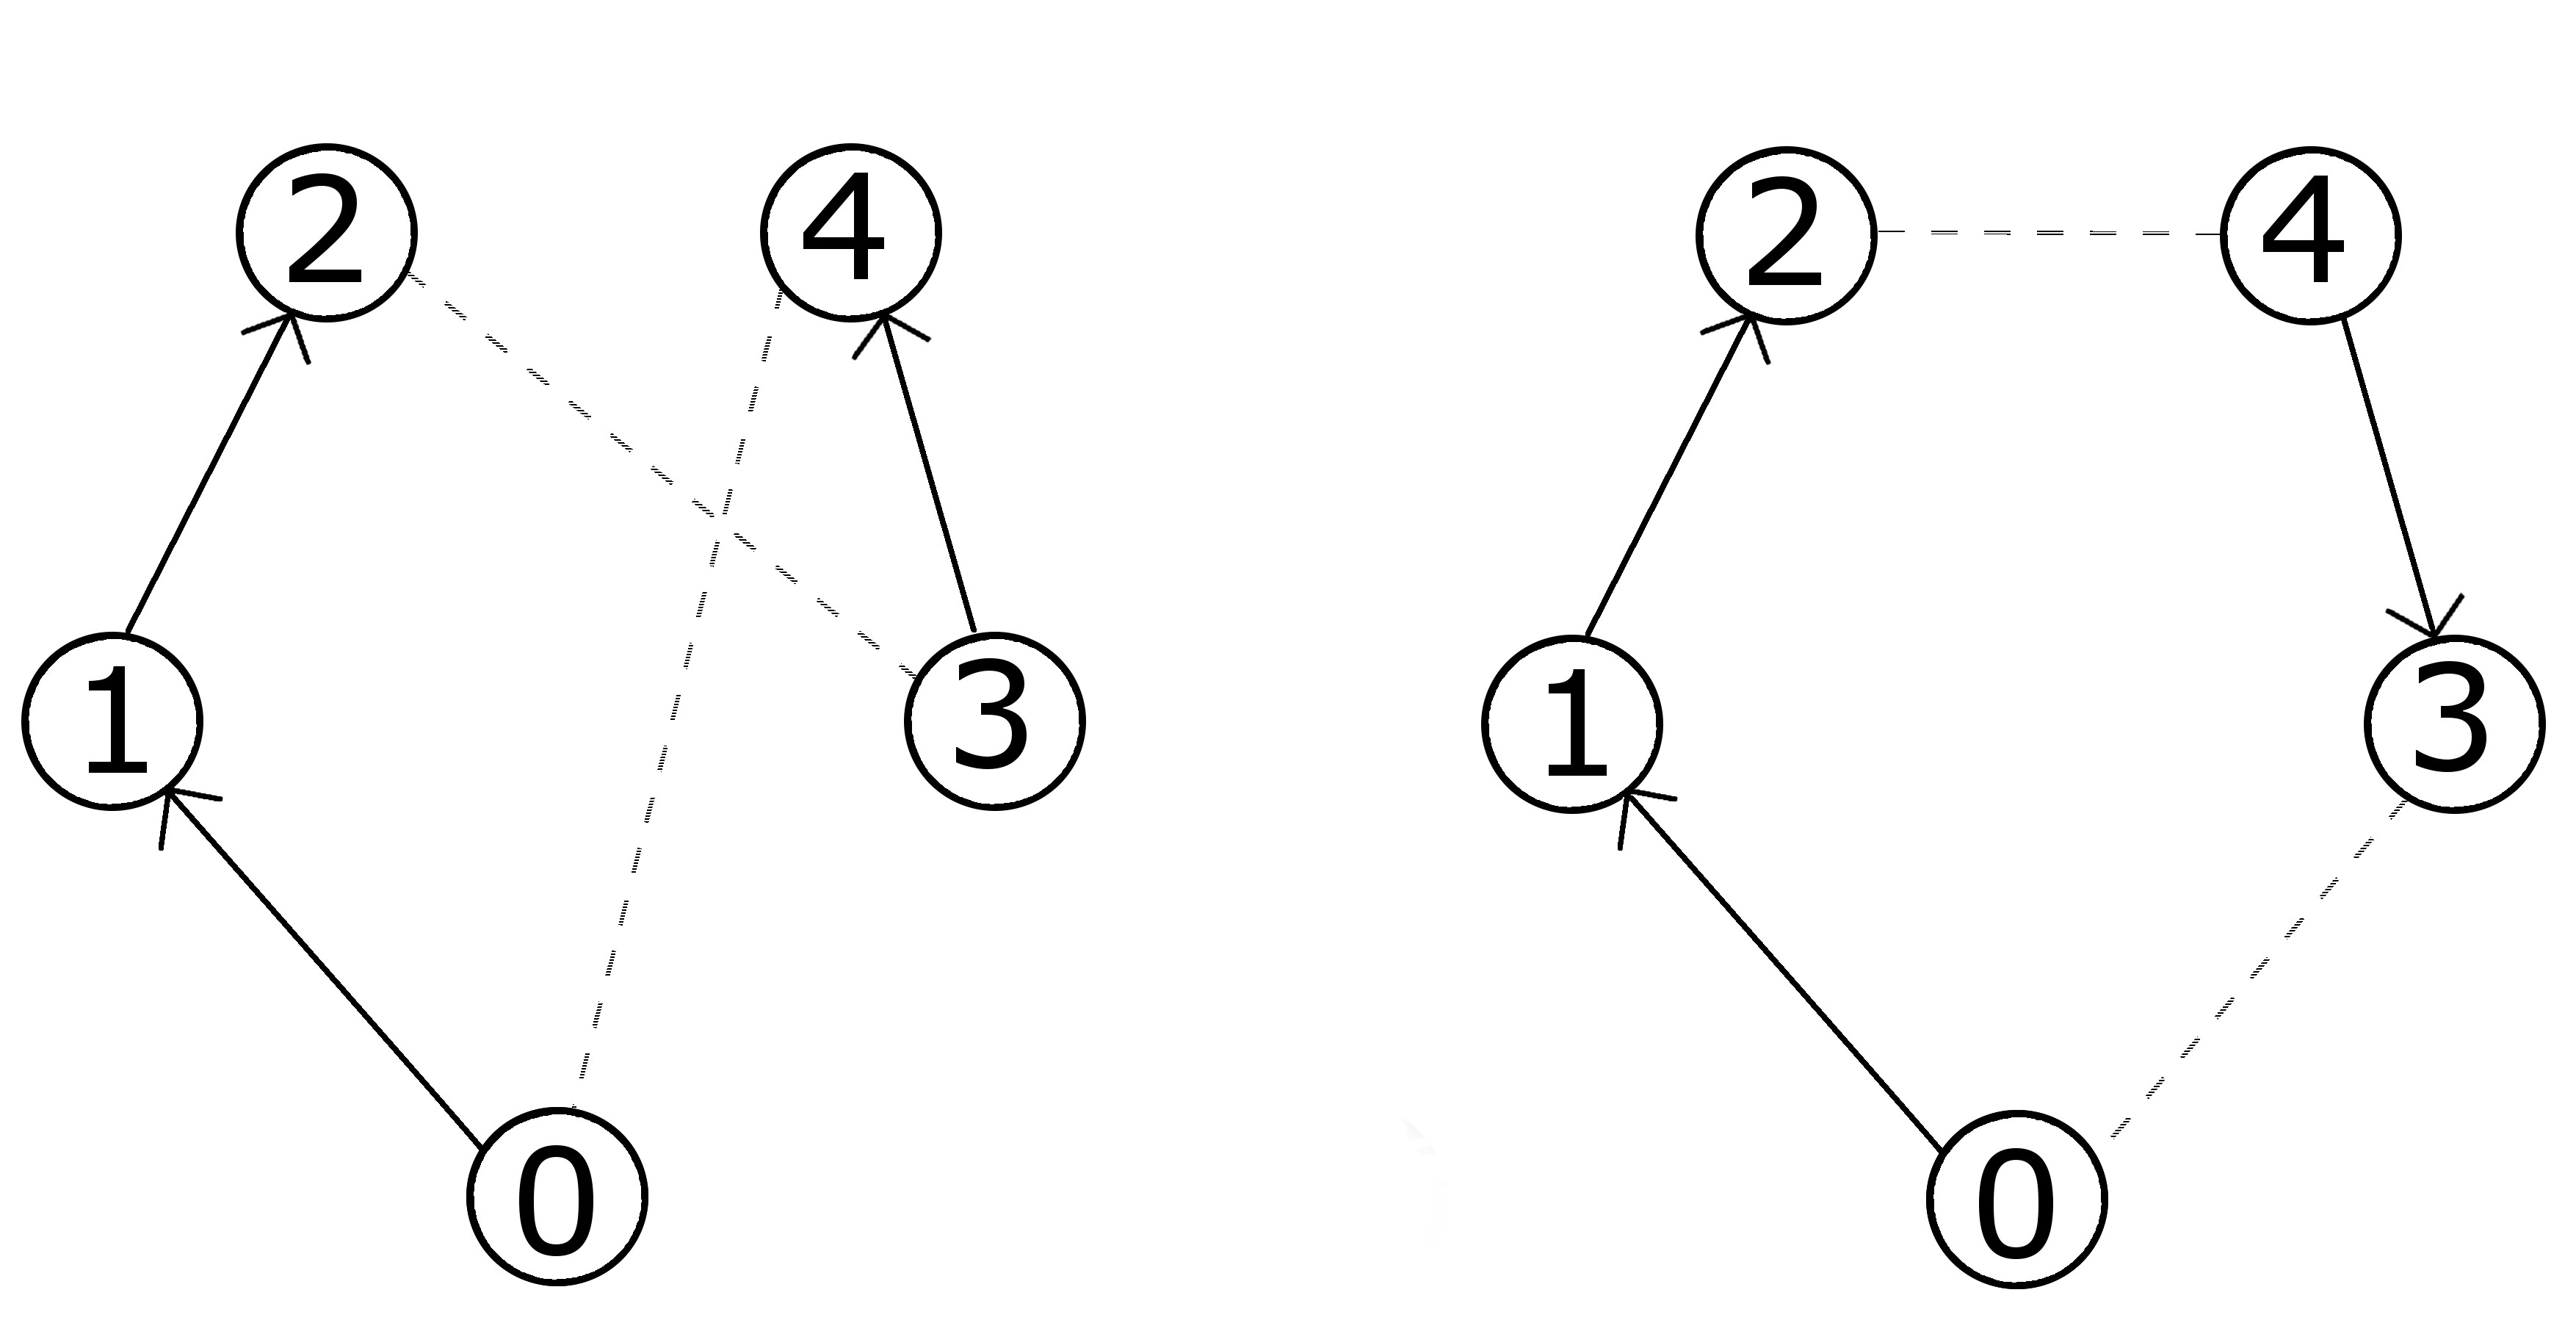
\includegraphics[width=\linewidth]{./img/lk1y2.jpg}
	}
	\caption{2-opt exchange.}
	\label{move1}
\end{figure}\

An implementation of the 2-opt algorithm usually perform exchanges until no saving moves can be done. In this way, this algorithm generates an initial tour, $\tau$, and performs exchanges to create new tours, $\hat{\tau}$, until $max(\alpha)<0$. When the algorithm ends the last created tour is the best found tour. A generalization of this simple principle forms the basis for the Lin-Kerninham algorithm. Lin and Kerninham realized that a 2-opt may stop at a local minimum because it does not allow negatives exchanges. In this way, if negatives exchanges are allowed to transform $\tau$ into $\hat{\tau}$ where the distance of $\hat{\tau}$ is bigger, i.e., $c(\tau) < c(\hat{\tau})$, and 2-opt moves are considered in $\hat{\tau}$, then a new tour $\hat{\tau}^{'}$ with shorter length than $\tau$ may be found. Moreover, Lin-Kerninham introduces a different stopping criteria. This algorithm does not allow to change moved arcs, in such a way, the algorithm will stop when every exchange involves moved arcs. The Lin-Kerninham algorithm can be implemented following the next steps:\\

%\fbox{%
%	\parbox{\textwidth\hspace{4pt}}{%
%		\begin{steps}{Step}
%			\step Generate a random initial tour, $\tau$, and set $j = 1$.

%	\begin{steps}{Step 2.}
%			\step Perform the best 2-opt exchanges of $\tau$ creating $\tau^{j}$ (even exchanges representing losses) and set $j = j + 1$.
%			\step Perform the best 2-opt exchanges of $\tau^{j-1}$ creating $\tau^{j}$ which does not modify created arcs at step 2.
%			\step	Repeat step 3 until exchanges cannot be performed.
%			\step Set $\tau^{'}$ such that $c(\tau^{'}) = min(c(\tau^{j}))$
%			\step If the distance of $\tau^{'} $ is smaller than the distance of $\tau$, then let $\tau = \tau^{'} $ and go to step 2.\\ If the distance of $\tau^{'}$ is greater or equal to the distance of $\tau$, then the algorithm ends. \label{step6}
%	\end{steps}


%		\end{steps}
%}}\\

Lets introduce the proposed modification of the algorithm, hereinafter referred to as exchange algorithm, after underlying that this modification will enhance routes instead of tours. Recall that the Lin-Kerninham algorithm was designed to solve traveling salesman problems, hence it is used to improve tours which do not have to respect VRPWT'S constraints. Capacity and time windows constraints may reduce the number of accomplished exchanges. That fact can guide the exchange algorithm to a local minimum, thus more moves must be considered. In this way, given a route, $r=(0,\dots,v_{i},\dots,v_{j},\dots,0)$, %of a routing configuration $\{r_{1},r_{2},\dots,r_{m}\}$, h  the algorithm will consider the 
the proposed modification considers the following exchanges:

$r=(v_{0},\dots,v_{i-1},v_{i},\dots,v_{j}, v_{j+1},\dots,v_{r+1})$ $\rightarrow_{move}$
$r^{'}=(v_{0},\dots,v_{i-1},v_{j},\dots,v_{i},v_{j+1},\dots,v_{r+1})$,

$\forall i = 1,\dots,|r| - 1$, $\forall j= i+1,\dots,|r| $.

That is, the algorithm can exchange any pair of customers visited by route $r$, while the original algorithm just considers to exchange consecutive customers of a route. Observe that the running time increases as the number of exchanges increase. Nerveless, the improvement of the solution by this modification justifies its small increasing of running time. Moving back to the traveling salesman problem, note that any move which does not involve modified arcs can be taken. However, the exchange algorithm chooses the best move and it checks whether the move can be taken. Therefore it can be said that the exchange algorithm chooses candidates. If the candidate respects the constraints the move is taken, otherwise the candidate will be rejected and the algorithm will select a different candidate. When a move is taken the route $r$ is transformed into a route $r^{'}$. In order to be able to select the best route, the exchange algorithm creates a list of improved routes.

The best candidate is the move which minimizes the cost of $r^{'}$. The difference of cost between routes $r$ and $r^{'}$ produced by exchanging nodes $v_{i}$ and $v_{j}$ is computed by $\alpha(v_{i},v_{j}) = c(v_{i-1},v_{i}) + c(v_{j},v_{j+1} ) - c(v_{i-1},v_{j} )- c(v_{i},v_{j+1})$. Note that whether $\alpha(v_{i},v_{j})>0$ the move represents savings, but if $\alpha(v_{i},v_{j})<0$ the move represents losses. Recall that the Lin-Kerninham algorithm chooses the best move, i.e., $max\{\alpha(v_{i},v_{j}), v_{i}, v_{j} \in \tau \} $ until no moves can be done, even moves representing losses. However, an implementation of the Lin-Kerninham algorithm which just considers saving moves has shown a quality outcome (\cite{Helsgaun}). Thus the exchange algorithm introduces this consideration. Moreover,the exchange algorithm incorporates a geometric biased distribution, $\beta$, to select candidates. The implemented randomization have been applied in \cite{Juan} showing good results. In this way, the exchange algorithm ends if no saving moves exist and candidates are chosen by a probabilistic parameter. 

To select a candidate, the exchange algorithm creates a matrix, $M$, whose columns represents, $v_i,v_j,$ $ \alpha(v_i,v_j)$ and whose dimension is $n \times 3$, where $n$ denotes number of possible moves. Once the matrix is sorted by $\alpha$ in decreasing order, its first row will represents the best move, while its last row will represents the worst one. The candidate will be selected from $M$ computing a value $m$, $m=\frac{\log(p)}{\log (1- \beta)}mod$ $n$, where $\beta  \in [0,1)$ and $p$ is a random number, $p \in (0,1]$. That is, setting a value of $\beta$ and randomly generating a value of $p$, $m$ will take a value in the interval $[1,n]$. After computing the value of $m$, the exchange algorithm considers the candidate as the move represented in the $m$ row of $M$. Note that since $p \in (0,1]$, if $\beta \rightarrow 1$ the algorithm will choose the best candidate and, if $\beta = 0$ the algorithm may choose one of the worst candidates. Furthermore, exchanges may represent losses if $\beta < 1$. Remember that the Lin-Kerninham algorithm does not allow moves which involves modified arcs, i.e, it does not allow to move exchanged nodes $v_{i}, v_{i+1},v_{i+2}, v_{i+3}$. This thought is a good approach but it may involve few iterations of the algorithm, which is not really a disadvantage when just the Lin-Kerninham algorithm is used to improve a tour. However, this Master thesis proposes a metaheuristic formed by three different local searches, thus each local search should have a good running time. The metaheuristic searches small improvements of the solutions at each iteration (subsection \ref{Mainalgorithm} details the main algorithm), thus each local search just needs to improve a given routing configuration,i.e., local searches do not try to find the optimal solutions. Furthermore, the exchange algorithm allows more moves than the Lin-Kerninham algorithm, which may need a different criteria to forbid moves. Hence, considering these ideas, the exchange algorithm does not allow to move exchanged nodes $v_i,v_j$ and it stops when no moves can be taken or the $max(M(\alpha))<0$.

To summaries, the exchange algorithm starts at an initial route, $r$, of a given routing configuration, computes the matrix $M$ and chooses a candidate by $m$. If the the candidate can be taken, its customers are exchanged transforming the route $r$ into a new route $r^{'}$. The algorithm inserts $v_i,v_j$ into a tabu list, $r^{'}$ into a list of improved routes and sets $r = r^{'}$. If the candidate cannot be taken, it is removed from $M$ and the algorithm selects other candidate recalculating $m$. The algorithm iterates over this logic until no moves can be taken, i.e., $max(M(\alpha))<0$ or the tabu list does not allow to exchange customers. 

When the algorithm meets these criteria, it chooses the best route, $ r^{'}$, from the list of improved routes and checks whether the cost of this route, $c( r^{'})$, is smaller than the cost of the initial route $c(r)$. If $c( r^{'}) < c(r)$, the initial route is setted as the best improved route and the algorithm starts again. Otherwise, the $r^{'}$ is not better than $ r$, thus the algorithm stops to improve the select route and selects a different one until all routes are analyses. %It must be underline that when the Lin-Kerninham algorithm's stopping criteria stops the algorithm, it sets the improved tour as the initial tour (see \ref{step6} of the algorithm). Nevertheless the proposed modification ends when the stopping criteria stops the iteration. The modification does not incorporate this step to find an improvement of a given solution instead of finding a nearly-optimal solution. However, one can see that iteratively executing the modification is equivalent to incorporate Step 6 to the modification.
The pseudo-code of the proposed modification is given bellow (algorithm \ref{opt}):


\begin{algorithm}[H]
\caption{exchange\_algorithm(initial\_routing\_configuration, $ \beta$ )}
\label{opt}
\begin{algorithmic}[1]
	\STATE routing configuration $\leftarrow$ initial routing configuration 																	  
	\FOR{ initial\_route in routing configuration}
	\WHILE{ stop\_route  $\ne$ 1 }
	\STATE route $\leftarrow$  initial\_route
	\WHILE{ stop\_iteration $\ne$ 1}
	\STATE compute $M$ 
	\WHILE{$max(M(\alpha))\geq 0$   and recalculate $\ne$ 1   }
	
	\STATE candidate  $\leftarrow$ compute\_m($\beta,p,n$)
	\IF{candidate respects constraints}
	\STATE route  $\leftarrow$  candidate 
	\STATE list\_improvements (route)  $\leftarrow$  route   
	\STATE recalculate $\leftarrow$ 1 
	\STATE tabu  $\leftarrow$    $(v_{i},v_{j})$  
	\ELSE 
	\STATE  remove candidate	from $M$
	\ENDIF
	\IF{ $max(M(\alpha))< 0$	or  length(tabu) $ \geq |r|-1$ }
	\STATE recalculate  $\leftarrow$ 1
	\STATE stop\_iteration  $\leftarrow$ 1
	\ENDIF
	\ENDWHILE
	\ENDWHILE
	
	\IF{ cost(best(list(route))) $\le$ cost(initial\_route) }
	\STATE initial\_route  $\leftarrow$ best(list(route))
	\STATE clear tabu	    
	\ELSE
	\STATE  stop\_route  $\leftarrow$ 1 
	\ENDIF
	\ENDWHILE
	\STATE routing configuration $\leftarrow$ initial\_route.
	\ENDFOR
	\STATE return(routing configuration) 
\end{algorithmic}

\end{algorithm}





\subsection{Inserting and swapping moves}\label{MovesDifferentRoutes}

This section details the moves between different routes which aim to minimize the number of routes and its cost. Given a routing configuration, $\{r_{1},r_{2},\dots,r_{m}\}$, the algorithm will consider, for each customer, two kind of movements: inserting and swapping changes. 
Inserting moves insert a customer $v_{i} \in r_{p}, p = 1,\dots,m-1$, into $r_{q}$ where $q=p+1,\dots,m$ as follows:

\begin{equation*}
\begin{rcases}
r_{p} &= (0,\dots,v_{i-1},v_{i},v_{i+1},\dots,0) \\
r_{q} &= (0,\dots,v_{j},v_{j+1},\dots,0)
\end{rcases}
\text{ $\rightarrow_{\text{inserting move}}$}	\begin{rcases}
r_{p} &= (0,\dots,v_{i-1},v_{i+1},\dots,0)\\
r_{q} &= (0,\dots,v_{j},v_{i},v_{j+1},\dots,0)
\end{rcases}
\end{equation*}
In other hand, swapping moves exchange a customers $v_i, v_j$ of different routes, that is, a swapping move can swap any customers $v_{i} \in r_{p}, p = 1,\dots,m-1$, $v_{j} \in r_{q}$ where $q= p + 1, \dots , m$  as follows:


\begin{equation*}
\begin{rcases}
r_{p} &= (0,\dots,v_{i-1},v_{i},v_{i+1},\dots,0)  \\
r_{q} &= (0,\dots,v_{j-1},v_{j},v_{j+1},\dots,0)
\end{rcases}
\text{ $\rightarrow_{swap}$}	\begin{rcases}
r_{p}^{'} &= (0,\dots,v_{i-1},v_{j},v_{i+1},\dots,0)  \\
r_{q}^{'} &= (0,\dots,v_{j-1},v_{i},v_{j+1},\dots,0)
\end{rcases}
\end{equation*}

Both inserting and swapping moves are represented by figure bellow (\ref{moves2}). This figure illustrates an example where a routing configuration is formed up by two routes $r_{1} = (0,3,4,0)$ and $r_{2} = (0,1,2,0)$. Letting $v_i = 2$ and $v_j = 4$. One can see at figure \ref{ExInsertingMove} that an inserting move can insert customer $4$ into $r_2$. On the other hand, figure \ref{ExSwappingMove} shows that a swapping move can swap these customers.

\begin{figure}[H]
\begin{subfigure}{.5\textwidth}
	\centering
	% include first image
	\includegraphics[width=.8\linewidth]{./img/join.jpg} 
	\caption{Inserting moves between different routes.}
	\label{ExInsertingMove}
\end{subfigure}
\begin{subfigure}{.5\textwidth}
	\centering
	% include second image
	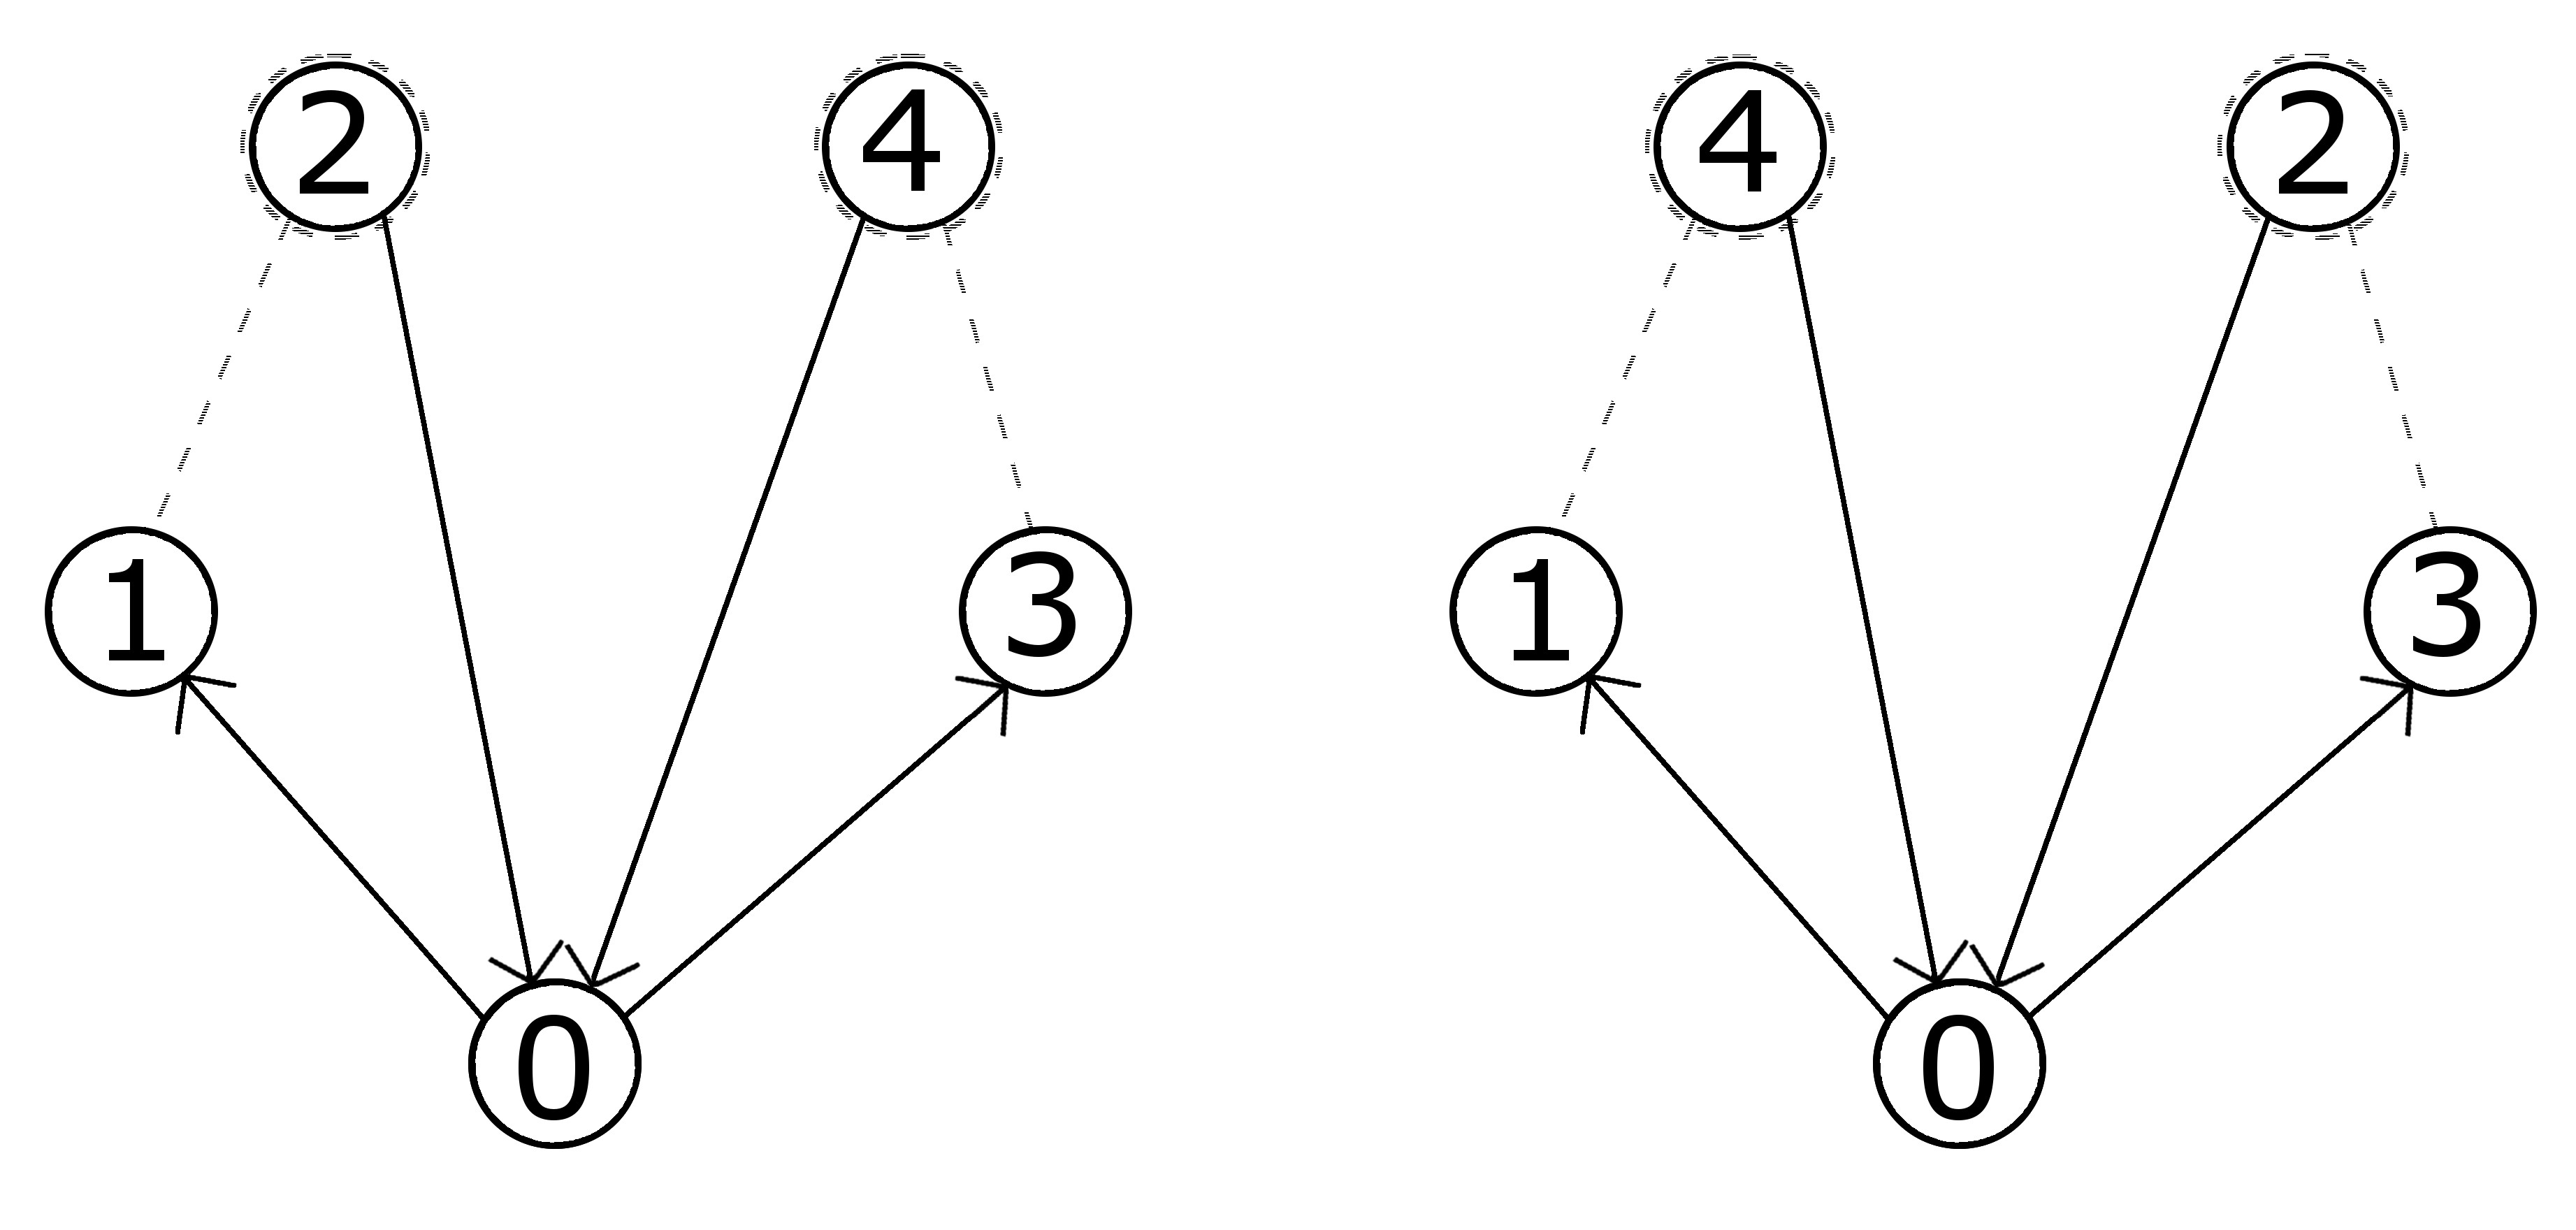
\includegraphics[width=.8\linewidth]{./img/swap.jpg} 
	\caption{Swapping moves different routes.}
	\label{ExSwappingMove}
\end{subfigure}
\caption{Moves between different routes}
\label{moves2}
\end{figure}


Both inserting and swapping moves may change the total cost of the routes. The difference of cost between routes $r_{p},r_{q}$ and routes $r_{p}^{'},r_{q}^{'}$ produced by inserting a customer $v_i$ of $r_p$ between customers $v_j, v_{j+1}$ of $r_q$ is denoted by $\alpha$ and its computed as follows:
$\alpha(v_{i},v_{j}) = c(v_{i-1},v_{i}) + c(v_{i},v_{i+1}) + c(v_{j},v_{j+1}) -c (v_{i-1},v_{i+1}) -c (v_{j},v_{i})- c(v_{i},v_{j+1})$.

%Figure \ref{moves3} shows this type of moves.
On the other side, the cost difference produced by swapping a customer $v_i$ of the route $r_p$ with a customer $v_j$ of the route $r_q$ can be computed by
$\alpha(v_{i},v_{j}) = c(v_{i-1},v_{i}) + c(v_{i},v_{i+1}) + c(v_{j-1},v_{j})  + c(v_{j},v_{j+1}) 
-c (v_{i-1},v_{j}) -c (v_{j},v_{i+1})- c(v_{j-1},v_{i}) -  c(v_{i},v_{j+1})$.

To implement these movements, two algorithms were developed: an inserting algorithm and a swapping algorithm. These algorithms enhance a given routing configuration by moves until a stopping criteria is met. These moves must respect VRPTW's constraints, thus the algorithms select candidates from all possible moves and perform the best candidate which respects VRPTW's constraints, that is, the best move which can be taken. As explained in \ref{MovesInsideRoutes}, these algorithms create a matrix, $M$, whose rows represents every possible move between any route of the configuration route and they select candidates by the value $m$, with random components. The algorithms stop when the stopping criteria is met, $max(M(\alpha))<0$. The main difference between exchange algorithm and inserting and swapping algorithms is that the exchange algorithm computes exchanges between customers of a route while the inserting and swapping algorithms perform moves between different routes. Thus, the exchange algorithm improves the routing configuration by enhancing its routes one by one while the inserting and swapping algorithms perform a global improvement.

Furthermore, the inserting and swapping algorithms modify the initial routing configuration. Recall that a routing configuration is formed up by a set of routes, $\{r_{1},r_{2},\dots,r_{m}\}$. The number of customer of each route can differ. In this sense, trying to insert a customer into a route which visits lot of customers is not likely to succeed, because it may violate time windows constraints. Besides, trying to insert a customer into a route which visits a few customers likely to succeed, because it probably does not violate time windows constraints. This consideration suggests to order a routing configuration by the length of its routes. In this way, given a routing configuration, the algorithms sort it by decreasing order creating a new one whose first route is the one which visits more customers, while its last route is the shortest one, i.e., $|cust(r_1)| \geq |cust(r_2)| \geq  \dots \geq  |cust(r_m)|$. In this way, if the inserting algorithm tries to insert a customer of the first route into the last one by setting $p=1$ and $q=m$, it probably finds a feasible insertion. This sorting criteria may unify the number of customer of the routes. Nevertheless, a stander objective for the VRPTW is to minimize the number of routes, thus trying to insert customers of small routes into large routes may decrease the number of routes. This objective suggests that the configuration route must be order in increasing order i.e., $|cust(r_1)| \leq |cust(r_2)| \leq   \dots \leq |cust(r_m)|$. Regarding these ideas, the inserting algorithm can sort a given routing configuration by increasing order and decreasing order.

To summaries, the inserting and swapping algorithms start at given routing configuration and the inserting one sorts the configuration by a given order. The algorithms compute the matrix $M$ and choose a candidate by $m$. If the the candidate can be taken, its customers are exchanged transforming the routing configuration $R$ into a new routing configuration $R^{'}$. The algorithms insert $R^{'}$ into a list of improved routing configurations and sets $R = R^{'}$. If the candidate cannot be taken, it is removed from $M$ and the algorithms select another candidate recalculating $m$. The algorithms iterate over this logic until no moves can be taken, i.e., $max(M(\alpha))<0$. When the algorithms meet these criteria, they choose the best routing configuration, $R^{'}$, from the list of improved routing configurations. Then algorithms check whether the cost of this routing configuration, $c(R^{'})$, is smaller than the cost of the previous routing configuration, $c(R)$. If $c(R^{'}) < c(R)$, then $R$ is setted as $R^{'}$ and the algorithms start again. Otherwise, the algorithms do not improve the solution, thus the algorithms stop. Note that inserting and swapping algorithm have the same logic but they are run separately.

The pseudo-code of the proposed modification is given bellow (algorithm \ref{insert}):

\begin{algorithm}[H]
\caption{swapping\_algorithm / inserting\_algorithm(initial\_routing\_configuration, $ \beta$, order\_criteria) }
\label{insert}
\begin{algorithmic}[1]
	
	\STATE routing configuration $\leftarrow$ sorted(initial routing configuration, order\_criteria) 													  
	\STATE stop\_algorithm  $\leftarrow$ 0
	
	\WHILE{ stop\_algorithm = 0}
	\STATE stop\_iter  $\leftarrow$ 0
	\WHILE{ stop\_iter $\ne$ 1}
	\STATE M  $\leftarrow$ compute\_M($p,n$)
	\STATE candidate\_inserted  $\leftarrow$ 0
	
	\WHILE{ candidate\_inserted = 0 and stop\_iter  $\ne$ 1}
	\STATE candidate $\leftarrow$ select candidate from M using $\beta$
	\STATE routing configuration  $\leftarrow$  candidate
	\IF {routing configuration respect constraints}
	\STATE list\_improvements(routing configuration)  $\leftarrow$  routing configuration
	\ELSE
	\STATE remove candidate from M
	\ENDIF
	\IF{ $max(M(\alpha))<0$}
	\STATE stop\_iter  $\leftarrow$ 1	    
	\ENDIF
	\ENDWHILE
	
	\IF {there are no\_improvements}
	\STATE stop\_algorithm  $\leftarrow$ 1
	\ENDIF
	
	\ENDWHILE
	\ENDWHILE
	
\end{algorithmic}

\end{algorithm}

\subsection{Main algorithm}\label{Mainalgorithm}

The proposed metaheuristic has been implement by a main algorithm which incorporates exchange, inserting and swapping algorithms. These three algorithms define local searches which are guided by the metaheuristic under different $\beta$ values.

In this sense, the metaheuristic computes one of the initial solutions detailed in subsection \ref{initialsol}. Once an initial solution is created, the metaheuristic improves it by iterating through the procedure. That is, given an initial solution, the metaheuristic enhances it by computing exchange moves of routes, inserting or swapping customers between routes. Each of these local searches may obtain different improved solutions, thus the metaheuristic chooses the best one and it sets the best improved solution as the new solution. This logic is repeated until a stopping criteria is met. The stopping criteria will be discuss after introducing some concepts. Recall that the local searches incorporates a probabilistic parameter $\beta$ and both inserting and swapping algorithms can order a given solution. In this way, the metaheuristic runs local searches under all possible sorting criteria: decreasing, increasing or no order. 

Let's analize the metaheuristic's behavior under different $\beta$ values. Recall that whether $\beta=1$ local searches must select the best move as candidate, while small $\beta$ values allow local searches to select candidates which do not represents big savings. Let $\beta=1$ and consider an initial solution, $R$, whose cost is noted by $c(R)$. Suppose that $R$ is being enhanced by a local search, for example, swapping algorithm. Remember that this algorithm creates a matrix $M$ which represents all swaps, where its first row represents the best move, the second row represents the second best move, etc. Then the swapping algorithm starts at $R$ and it performs the best swap creating $R_{1}$ such that $c(R_{1}) \leq c(R)$. After this swap, the algorithm may finish because no swap which represents savings can be taken. However, if $\beta<1$ a different move can be taken, for example the second best move. Selecting the second candidate, the algorithm creates a new route $R_{2}$ such that, $c(R_{1}) \leq c(R_{2}) \leq c(R)$. After this move, the algorithm is more likely to find other swap which represents savings. Thus, a second swap can be taken computing a route $R_{3}$ such that $c(R_{3})\leq c(R_{1}) \leq c(R_{2}) \leq c(R)$. Thus, if $\beta = 1$, a local search can stop at a local minimum, while if $\beta <1$ the local search may find better solutions. One can find that this logic is very similar to the one implemented by Lin and Kerninham, which was explained at subsection \ref{MovesInsideRoutes}. Furthermore, if $\beta$ is small enough, the local searches may select candidates which represent losses. Taking these candidates may do not seem good a good idea but it can help to explore different solutions.

The proposed metaheuristic incorporates this consideration by starting to iterate with small $\beta$ values. To test the metaheuristic behavior, first iterations are run with $\beta = 0.6$, allowing the local searches to choose negative moves. Once no improvements are found by local searches, the metaheuristic sets $\beta = 0.8$, in order to find better solutions. Under this $\beta$ value, the local searches may not select negative moves but they do not have to select the best candidate. When no improvements are found under $\beta = 0.8$ the metaheuristic change to $\beta=1$ to refine the final solution. Once no improvements are found, the metaheuristic ends approximating the optimum of the problem by the last found solution, $R^{'}$. A metaheuristic may provide a sufficiently good solution, but it may be improved. One can think that proposed metaheuristic can enhanced $R^{'}$ by setting $\beta<1$ again. That is probably true, however, it is not certain that the probabilistic parameter did not guide the local search to a local minimum. Thus, the metaheuristic must end if $\beta = 1$ and the local search do not improve the solution. These considerations form the stopping criteria. If one wants to obtain a better solution than $R^{'}$, the metaheuristic must be run again starting from one of the initial solutions detailed in subsection \ref{initialsol}. The pseudo-code of the proposed metaheuristic is given at the end of these section (algorithm \ref{main}).


Observe that the proposed metaheuristic runs the local searches individually to evaluate three different moves: exchanges, insertions or swaps. That is, the metaheuristic gives a solution, $R$, to every local search and it chooses the best improved solution, $R^{'}$. What means that $R$ is improved by one kind of move. Lets evaluate how the proposed metaheuristic combines the different moves. Suppose that the metaheuristic is started at a dummy solution and recall that dummy solution's routes only visit one customer. In this routing configuration, the time window constraints are soft constraints, thus the inserting algorithm can reduce the number of routes. Hence, at first iterations, inserting algorithm performs the best improvements. After a few iterations, the routes of the improved solution visit few customers, thus the time windows constraints may allow to perform some insertions. Since the routes visit few customers the exchange algorithm can reduce the routes' cost. Furthermore, the inserting algorithm could has made insertions which guide the metaheuristic local minimum. However, the swapping algorithm can break them up at these iterations. In this situation, the three local searches can improve the actual solution. At last iterations of the metaheuristic, the local searches must improve a routing configuration whose routes visit lot of customers, which implies that time windows constraints are strong constraints. Hence, exchange and swapping algorithms may offer the best improvements. On the other hand, if an elaborated initial solution is considered, every local search have a main role in the metaheuristic. Observe that swapping algorithm can reconfigure the clustered customers if it is needed.

\begin{algorithm}[H]
\caption{Metaheuristc}
\label{main}
\begin{algorithmic}[1]
	\STATE solution $\leftarrow$ initial solution
	\STATE iter $\leftarrow$ 1
	\STATE $\beta_{values} \leftarrow (0.6, 0.8, 1)$          																	  
	\WHILE{ iter	$<$ len(beta)}
	\STATE $\beta \leftarrow \beta_{values}(iter)$
	\STATE no\_improvement  $\leftarrow$ 0
	\WHILE{ no\_impromevement	  $\ne$ 1 }
	\STATE  list(solutions) $ \leftarrow$ inserting\_algorithm(solution, $\beta$, order = decreasing)			
	\STATE  list(solutions) $ \leftarrow$ inserting\_algorithm(solution, $\beta$, order = increasing)			
	\STATE  list(solutions) $ \leftarrow$ swapping\_algorithm(solution, $\beta$)				
	\STATE  list(solutions) $ \leftarrow$ exchange\_algorithm(solution,$\beta$)							
	\STATE  new solution $ \leftarrow$ best( list(solutions))
	\IF{ new solution is better than solution}
	\STATE solution $\leftarrow$ new solution
	\STATE clear (list(solutions)) 
	\ELSE 
	\STATE  no\_improvement $\leftarrow$  1 
	\ENDIF
	\ENDWHILE
	\STATE iter $\leftarrow$ iter + 1 
	\ENDWHILE
	\STATE return (solution)
\end{algorithmic}
\end{algorithm}



\section{Computational results}\label{results}
This section describes experimental results obtained with the proposed metaheuristic, which was coded in Python and run on an $Intel^{\textsuperscript{\textregistered}}$ $Core^{TM}$ i7-8750H at 2.20GHz and 16BG RAM. The metaheuristic was tested with Solomon benchmark problems and at a real agricultural cooperative problem.

\subsection{Solomon benchmark}
Computational results has been conducted to compare the perform of the proposed metaheuristic, which has been tested with 56 VRPTW benchmark problems of Solomon (1987). 

These instances are widely used in the literature. Each problem involves 100 customers, distributed over a square $[0,100]^{2}$ in the plane. Customer locations for a those instances are either generated randomly using an uniform distribution, data sets R1 and R2, clustering customers (data sets C1 and C2) or combining randomly distributed and clustered customers (data sets RC1 and RC2).
Distances are represented by Euclidean distance and speed of all vehicles is assumed to be unity. That is, it takes one unit of time to travel one unit of distance. Distance and time are calculated with double precision and total distance results are rounded to two decimals. Instances and best known solutions were obtained at this \href{https://www.sintef.no/projectweb/top/vrptw/solomon-benchmark/100-customers/}{link}. 

The metaheuristic was executed setting $\beta = (0.6, 0.8, 1)$ and starting from an elaborated initial solution. Tables \ref{TABLE-BKS1}, \ref{TABLE-BKS2}, \ref{TABLE-BKS3} compares the best known solutions and the solutions obtained by the proposed metaheuristic. The metaheuristic was executed starting from a dummy solution with some instances. Its results were similar to the ones obtained starting from an elaborated initial solution, but it was much time-consuming. Thus the whole Solomon data set was executed from an elaborated initial solution.

The metaheuristic offers good results at data sets C1 and C2. Setting $\beta = (0.6, 0.8, 1)$, it reaches the minimum number of routes to 13 data set out of 16 and it has a GAP of 4.22$\%$ . However, the metaheuristic must be executed with different $\beta$ values to get the best results. Section \ref{Robustness} gathers that analysis showing the metaheuristic gets its best results with $\beta = (0.2, 0.8, 1)$. Under that $\beta $ value the metaheuristic reaches the minim number of routes to all data sets and it has a GAP of 1.62$\%$. Results are gathered in the table bellow (\ref{BKS_soloutionC})

\clearpage

\begin{table}[H]
  \begin{tabular}{c c c c | c c c c}  

\hline
  \multicolumn{4}{c|}{Best known solution} & 	\multicolumn{4}{c}{Obtained solution} \\  
\hline
  Data set  &  N \textordmasculine routes & Distance & Author &  N \textordmasculine routes & Distance & GAP by distance (\%) & time (s)\\  
  \textbf{ c101} & \textbf{ 10} & 828.94 & RT & \textbf{10} & 828.94 & 0.0 & 193.0\\  
  \textbf{ c102} & \textbf{ 10} & 828.94 & RT & \textbf{10} & 835.28 & 0.76 & 286.0\\  
  \textbf{ c103} & \textbf{ 10} & 828.06 & RT & \textbf{10} & 886.64 & 7.07 & 1036.0\\  
  \textbf{ c104} & \textbf{ 10} & 824.78 & RT & \textbf{10} & 840.0 & 1.85 & 2259.0\\  
  c105 & 10 & 828.94 & RT & 11 & 900.45 & 8.63 & 1239.0\\  
  \textbf{ c106} & \textbf{ 10} & 828.94 & RT & \textbf{10} & 828.94 & 0.0 & 570.0\\  
  \textbf{ c107} & \textbf{ 10} & 828.94 & RT & \textbf{10} & 828.94 & 0.0 & 689.0\\  
  c108 & 10 & 828.94 & RT & 12 & 974.65 & 17.58 & 1266.0\\  
  \textbf{ c109} & \textbf{ 10} & 828.94 & RT & \textbf{10} & 852.76 & 2.87 & 793.0\\  
  \textbf{ c201} & \textbf{ 3} & 591.56 & RT & \textbf{3} & 591.56 & 0.0 & 214.0\\  
  \textbf{ c202} & \textbf{ 3} & 591.56 & RT & \textbf{3} & 620.29 & 4.86 & 776.0\\  
  c203 & 3 & 591.17 & RT & 4 & 683.9 & 15.69 & 767.0\\  
  \textbf{ c204} & \textbf{ 3} & 590.6 & RT & \textbf{3} & 635.64 & 7.63 & 1048.0\\  
  \textbf{ c205} & \textbf{ 3} & 588.88 & RT & \textbf{3} & 588.88 & 0.0 & 724.0\\  
  \textbf{ c206} & \textbf{ 3} & 588.49 & RT & \textbf{3} & 588.49 & 0.0 & 476.0\\  
  \textbf{ c207} & \textbf{ 3} & 588.29 & RT & \textbf{3 }& 591.73 & 0.58 & 507.0\\  
\hline

  \end{tabular} 
  \caption{BKS compared to obtained solution to data set C1 and C2.}  
\label{TABLE-BKS1}
\end{table}
\begin{table}[H]
  \begin{tabular}{c c c c | c c c c}  

\hline
  \multicolumn{4}{c|}{Best known solution} & 	\multicolumn{4}{c}{Obtained solution} \\  
\hline
  Data set  &  N \textordmasculine routes & Distance & Author &  N \textordmasculine routes & Distance & GAP distance & time (s)\\  
  r101 & 19 & 1650.8 & H & 22 & 1799.32 & 9.0 & 3359.0\\  
  r102 & 17 & 1486.12 & RT & 18 & 1611.6 & 8.44 & 5699.0\\  
  r103 & 13 & 1292.68 & LLH & 15 & 1363.32 & 5.46 & 2824.0\\  
  r104 & 9 & 1007.31 & MBD & 12 & 1099.33 & 9.14 & 1634.0\\  
  r105 & 14 & 1377.11 & RT & 15 & 1444.79 & 4.91 & 2974.0\\  
  r106 & 12 & 1252.03 & MBD & 14 & 1314.9 & 5.02 & 1799.0\\  
  r107 & 10 & 1104.66 & S97 & 12 & 1167.99 & 5.73 & 1724.0\\  
  r108 & 9 & 960.88 & BBB & 10 & 1080.84 & 12.48 & 1548.0\\  
  r109 & 11 & 1194.73 & HG & 13 & 1278.93 & 7.05 & 2780.0\\  
  r110 & 10 & 1118.84 & MBD & 13 & 1282.58 & 14.63 & 1525.0\\  
  r111 & 10 & 1096.72 & RGP & 12 & 1167.84 & 6.48 & 1691.0\\  
  r112 & 9 & 982.14 & GTA & 11 & 1091.5 & 11.13 & 1361.0\\  
  \textbf{ r201} & \textbf{ 4} & 1252.37 & HG & \textbf{4} & 1299.92 & 3.8 & 2348.0\\  
  r202 & 3 & 1191.7 & RGP & 4 & 1210.41 & 1.57 & 1936.0\\  
  \textbf{ r203} & \textbf{ 3} & 939.5 & WL & \textbf{3} & 1073.61 & 14.27 & 1187.0\\  
  r204 & 2 & 825.52 & BVH & 3 & 881.88 & 6.83 & 1206.0\\  
  \textbf{ r206} & \textbf{ 3} & 906.14 & SSSD & \textbf{3} & 1032.85 & 13.98 & 1131.0\\  
  r207 & 2 & 890.61 & RP & 3 & 935.75 & 5.07 & 1016.0\\  
  r208 & 2 & 726.82 & MBD & 3 & 792.47 & 9.03 & 595.0\\  
  r209 & 3 & 909.16 & H & 4 & 926.38 & 1.89 & 1031.0\\  
  \textbf{ r210} & \textbf{ 3} & 939.37 & MBD & \textbf{3} & 1017.49 & 8.32 & 1797.0\\  
\hline

  \end{tabular} 
  \caption{BKS compared to obtained solution to data set R1 and R2.}  
\label{TABLE-BKS2}
\end{table}
\begin{table}[H]
  \begin{tabular}{c c c c | c c c c}  

\hline
  \multicolumn{4}{c|}{Best known solution} & 	\multicolumn{4}{c}{Obtained solution} \\  
\hline
  Data set  &  N \textordmasculine routes & Distance & Author &  N \textordmasculine routes & Distance & GAP distance & time (s)\\  
  rc102 & 12 & 1554.75 & TBGGP & 16 & 1670.68 & 7.46 & 1693.0\\  
  rc103 & 11 & 1261.67 & S98 & 13 & 1429.66 & 13.31 & 2091.0\\  
  rc104 & 10 & 1135.48 & CLM & 12 & 1324.34 & 16.63 & 1211.0\\  
  rc105 & 13 & 1629.44 & BBB & 18 & 1752.04 & 7.52 & 2324.0\\  
  rc106 & 11 & 1424.73 & BBB & 14 & 1523.64 & 6.94 & 2420.0\\  
  rc107 & 11 & 1230.48 & S97 & 13 & 1430.89 & 16.29 & 1220.0\\  
  rc108 & 10 & 1139.82 & TBGGP & 12 & 1191.89 & 4.57 & 1543.0\\  
  \textbf{ rc201} & \textbf{ 4} & 1406.94 & MBD & 4 & 1769.74 & 25.79 & 1095.0\\  
  rc202 & 3 & 1365.65 & GCC & 4 & 1419.35 & 3.93 & 1138.0\\  
  rc203 & 3 & 1049.62 & CC & 4 & 1125.4 & 7.22 & 1397.0\\  
  \textbf{ rc204} & \textbf{ 3} & 798.46 & MBD & 3 & 933.83 & 16.95 & 631.0\\  
  rc205 & 4 & 1297.65 & MBD & 5 & 1471.13 & 13.37 & 1390.0\\  
  rc206 & 3 & 1146.32 & H & 4 & 1279.47 & 11.62 & 1504.0\\  
  \textbf{ rc207} & \textbf{ 3} & 1061.14 & BVH & 3 & 1212.43 & 14.26 & 1017.0\\  
  \textbf{ rc208} & \textbf{ 3} & 828.14 & IKMUY & 3 & 954.79 & 15.29 & 1085.0\\  
\hline

  \end{tabular} \  
  \caption{BKS compared to obtained solution to data set RC1 and RC2.}  
\label{TABLE-BKS3}
\end{table}\


\begin{table}[H]
\centering
\begin{tabular}{c | c c  | c c c }
\hline
\multicolumn{1}{c|}{}  & \multicolumn{2}{c|}{ Best known solution} & \multicolumn{3}{c}{ beta = (0.2, 0.8, 1)}\\
\hline
Data set  &  N \textordmasculine routes & Km &  N \textordmasculine routes & Km & GAP\\
\hline
C101.txt & 10 & 828.94  & 10 & 828.94 & 0.0     \\
C102.txt & 10 & 828.94  & 10 & 835.28 & 0.76    \\
C103.txt & 10 & 828.06  & 10 & 831.74 & 0.44   \\
C104.txt & 10 & 824.78  & 10 & 885.64 & 6.87    \\
C105.txt & 10 & 828.94  & 10 & 868.78 & 4.59    \\
C106.txt & 10 & 828.94  & 10 & 828.94 & 0.0    \\
C107.txt & 10 & 828.94  & 10 & 828.94 & 0.0     \\
C108.txt & 10 & 828.94  & 10 & 828.94 & 0.0    \\
C109.txt & 10 & 828.94  & 10 & 886.71 & 6.52    \\
C201.txt & 3 & 591.56   & 3 & 591.56 & 0.0     \\
C202.txt & 3 & 591.56   & 3 & 591.56 & 0.0     \\
C203.txt & 3 & 591.17   & 3 & 604.91 & 2.27     \\
C204.txt & 3 & 590.6    & 3 & 618.9 & 4.57     \\
C205.txt & 3 & 588.88   & 3 & 588.88 & 0.0     \\
C206.txt & 3 & 588.49   & 3 & 588.49 & 0.0     \\
C207.txt & 3 & 588.29   & 3 & 588.29 & 0.0     \\
C208.txt & 3 & 588.32   & 3 & 588.32 & 0.0     \\
\hline
\end{tabular} \
\caption{Best solution foun for C1 and C2 instances}
\label{BKS_soloutionC}
\end{table}\



\subsection{Agricultural cooperative}\label{results-AIRA}

This experiment considers a problem faced on (\cite{Balbina}) by a hybrid heuristic algorithm. This problem aims to minimise transportation costs of an agricultural cooperative.
The cooperative is formed by 15000 farmers located in Galicia, a region of Spain. Farmers demand different kinds of food from the cooperative once or twice a month. Farmer's demand have time windows. Orders can be urgent, which implies that they must supplied the same day.
Furthermore, the cooperative has a heterogeneous fleet of trucks which cannot travel more than a given number of kilometers per day. Trucks can carry food in their hoppers, which have different capacity. Furthermore drivers are paid in terms of distance traveled and load. 

This problem can be modeled by a incapacitated vehicle problem with time windows and heterogeneous fleet thus it can be faced by the proposed algorithm, which will try to minimize the number of routes and maximize truck's load. Different data sets are considered at \cite{Balbina}: a fictitious example, a small instance of real data and two instances of real data which include demands of two days.

\subsubsection{Fictitious example}

This example considers a fleet of two trucks: a small truck with two hoppers that can hold up to four and three tonnes of feed and a large truck with three hoppers, whose capacities are five, four and four tonnes. The first truck can not carry more than 6 tonnes and the large one can carry up to 20 tonnes at a time. These trucks must supply with one type of feed six farmers located in Ourense, Begonte, Friol, Sarria, A Estrada and Forcarei. Lets suppose trucks can perform a route per day. Tables \ref{demand1} and \ref{distance1} provide the parameters of the problem while traveling costs involve the following parameters (\cite{Balbina}):
\begin{itemize}
\item Maximum distance for trucks: 600 km.
\item Unloading cost: 2 euros per delivery.
\item Fixed transport cost: 1 euro per tonne carried.
\item Variable transport cost: 
\subitem Route traveling up to 100 km: 0.5 euros per km per tonne carried.
\subitem Route traveling up to 200 km: 0.75 euros per km per tonne carried.
\subitem Route traveling up to 300 km: 1 euros per km per tonne carried.
\end{itemize}

\begin{table}[H]
\centering
\begin{tabular}{c| c c c c c}
	\hline 
	%	\centering		
	Tonnes  	& Feed 1 & Feed 2   & Feed 3   &  Feed 4  &  Days left to deliver \\
	\hline 
	Ourense    	& & & 4.5 & & 1   \\
	Begonte  	& 4 & & & & 1    \\
	Friol    	& & 3 & & & 1    \\
	Sarria  	& & & & 4 & 3    \\
	A Estrada 	& & & & 3.5&  1  \\
	Forcarei	& 2.5 & & & &  2 \\
	\hline 
\end{tabular}

\caption{Farmers' demand.}
\label{demand1}
\end{table}\

\begin{table}[H]
\centering
\begin{tabular}{c| c c c c c c c}
	\hline 
	%	\centering		
	km/min  	& Coop & Ourense  & Begonte   &  Friol  &  Sarria   & A Estrada & Forcarei\\
	\hline 
	Coop 		& 	0  & 50/47   &  61/60    &  44/41  &  46/46    &  85/69   & 70/67 \\
	Ourense    	& 	   & 0/0     &  111/104  &  93/86  &  78/77    &  96/62   & 81/60 \\
	Begonte  	& 	   &         &  0/0      &  19/20  &  56/44    &  116/97  & 156/105 \\
	Friol    	& 	   &         &           &  0/0    &  57/55    &  103/90  & 92/89 \\
	Sarria  	&	   &         &           &         &  0/0      &  144/115 & 129/113 \\
	A Estrada 	&	   &         &           &         &           &  0/0     & 20/17 \\
	Forcarei	&	   &         &           &         &           &          & 0/ 0 \\
	\hline 
\end{tabular} \
\caption{Distances and traveling times between pairs of stockbreeders and depot.}
\label{distance1}
\end{table}\

The following solution is obtained after execute the proposed metaheuristic one minute:

\begin{itemize}
\item The small truck starts its route at depot, goes to Begonte, Sarria and goes back to the depot.
\item The big truck starts its route at depot, goes to Ourense, Forcarei, A Estrada and goes back to the depot.
\item The farmer from Sarria is not visited the first day.
\end{itemize}

This routing configuration satisfies cooperative's requirements offering solution 456 km.

\subsubsection{Small example}

This example considers a fleet of two trucks with five hoppers that can contain up to 3, 3.7, 3.8, 3.7 and 3 tonnes. Trucks can not carry more than 11.6 tonnes and just can perform a route per day. These trucks must supply, with one type of feed, five farmers with urgent orders of one kind of food. Moreover, both trucks can visit all customers. Table \ref{demand2} shows demand and urgency.


\begin{table}[H]
\centering
\begin{tabular}{c| c c }
	\hline 
	%	\centering		
	Tonnes  	& Feed 1 & Days left to deliver \\
	\hline 
	Farmer 1 &  3.3   & 1	\\
	Farmer 2 &  2.951 & 1	\\
	Farmer 3 &  3.003 & 1 \\
	Farmer 4 &  3.016 & 1	\\
	Farmer 5 &  2.496 & 1 \\
	\hline 
\end{tabular}
\caption{Farmers' demand.}
\label{demand2}
\end{table}\


The following solution is obtained after execute the proposed metaheuristic one minute minimizing the travel cost:

\begin{itemize}
\item First truck starts its route at depot, goes to farmer 1, farmer 4 and goes back to the depot.
\item Second truck starts its route at depot, goes to farmer 2, farmer 3, farmer 5 and goes back to the depot.

\end{itemize}

This routing configuration satisfies cooperative's requirements offering solution 221 km.


\subsubsection{Real examples}

This subsection considers a fleet of two different trucks with five hoppers. The maximum capacity of the hoppers of one truck are 3, 3, 1.7 4.5 and 3 tonnes, while other can contain up to 3, 3.7, 3.8, 3.7 and 3 tonnes. Trucks can not carry more than 15.3 tonnes. Three different sets of orders are considered in this section, which contains demands of 17, 19 and 36 farmers. To supply 36 farmers, fleet is doubled. Table \ref{distancereal} provide an overview of the obtained solutions.


\begin{table}[H]
\centering
\begin{tabular}{c| c c c c}
	\hline 
	%	\centering		
	Data	&	Distance (km)	&	N\textordmasculine routes & N\textordmasculine truck & Time(s)	\\
	\hline
	17 farmers	&	492	&	9	&	2&	64\\
	19 farmers	&	385	&	10	&	2&	164\\
	36 farmers	&	922	&	16	&	4&	1419 \\
	\hline 
\end{tabular} \
\caption{Results real instances.}
\label{distancereal}
\end{table}\


\clearpage

\section{Robustness}\label{Robustness}

Robustness is a desirable property of local search algorithms. An algorithm is robust if it performs well on large classes of problems with the same parameter configuration (\cite{Bent}). 

In order to analyze the metaheuristic's behavior, it was executed to solve Solomon's C1 and C2 instances. It was initialized at an elaborated initial solution and executed with different $\beta$ values, as mean to analyze its behavior under different probabilistic configuration. The first execution corresponds to $\beta = (1)$, which does not introduce random sampling. Second execution corresponds to $\beta = (0.8, 1)$, which allows the metaheuristics to choose one of the best moves. This execution finally sets up $\beta = 1$ to refine the solution. On the contrary, the last execution to $\beta = (0.2, 1)$, which allows the metaheuristics to choose any moves, including the worst moves. The other executions varies $\beta$ values from small values to large ones.

Tables \ref{solomon_beta_values} and\ref{solomon_beta_values2} gather the results of these executions. The metaheuristic performs its best results when $\beta = (0.2, 0.8, 1)$ to both C1 and C2 instances, that is, when then algorithm is randomized. It always reaches the minimum number of trucks and the GAP average to C1 instances is 2.13$\%$ and to C1 instances is 0.85$\%$. The average GAP between all execution is 4.04$\%$ to C1 instances and 4.10$\%$ to C2 instances. Thus the metaheuristic performs well on both data set with the same parameter configuration. 

\begin{table}[H]
\centering
\begin{tabular}{c | c c  | c c c  | c c c  }
\hline
\multicolumn{1}{c|}{} & \multicolumn{2}{c|}{ BKS} & \multicolumn{3}{c|}{ beta = (1)} & \multicolumn{3}{c}{ beta = (0.8, 1)}\\
\hline
 Data set  &  N \textordmasculine routes & Km &  N \textordmasculine routes & Km & GAP &  N \textordmasculine routes & Km & GAP\\
\hline
C101.txt & 10 & 828.94  & 10 & 828.94 & 0.0  	& 10 & 828.94  & 0.0 \\
C102.txt & 10 & 828.94  & 10 & 835.28 & 0.76  	& 10 & 835.28  & 0.76 \\
C103.txt & 10 & 828.06  & 10 & 976.0  & 15.16 	& 10 & 1065.65 & 22.3 \\
C104.txt & 10 & 824.78  & 10 & 865.7  & 4.73  	& 10 & 963.18 & 14.37 \\
C105.txt & 10 & 828.94  & 10 & 828.94 & 0.0  	& 10 & 833.24 & 0.52 \\
C106.txt & 10 & 828.94  & 10 & 833.24 & 0.52  	& 10 & 828.94 & 0.0 \\
C107.txt & 10 & 828.94  & 11 & 904.17 & 8.32  	& 10 & 828.94 & 0.0 \\
C108.txt & 10 & 828.94  & 10 & 915.12 & 9.42  	& 10 & 828.94 & 0.0 \\
C109.txt & 10 & 828.94  & 11 & 868.16 & 4.52  	& 11 & 866.04 & 4.28 \\
\hline
Average &  &  &  &4.82 &  & & &  4.69\\
\hline
C201.txt & 3 & 591.56  & 3 & 591.56 & 0.0  	& 3 & 591.56 & 0.0 \\
C202.txt & 3 & 591.56  & 3 & 591.56 & 0.0  	& 3 & 591.56 & 0.0 \\
C203.txt & 3 & 591.17  & 3 & 604.58 & 2.22  & 3 & 591.17 & 0.0 \\
C204.txt & 3 & 590.6   & 3 & 664.98 & 11.19 & 3 & 677.68 & 12.85 \\
C205.txt & 3 & 588.88  & 3 & 603.48 & 2.42  & 3 & 588.88 & 0.0 \\
C206.txt & 3 & 588.49  & 4 & 663.84 & 11.35 & 4 & 626.2 & 6.02 \\
C207.txt & 3 & 588.29  & 4 & 622.63 & 5.52  & 4 & 618.37 & 4.86 \\
C208.txt & 3 & 588.32  & 3 & 588.32 & 0.0   & 3 & 600.88 & 2.09 \\
\hline
Average &  &  &  &4.08 &  & & &  3.21\\
\hline
\end{tabular} \
\caption{BKS setting different beta values}
\label{solomon_beta_values}
\end{table}


\clearpage
\begin{table}[H]
\centering
\begin{tabular}{c | c c  | c c c  | c c c  }
\hline
\multicolumn{1}{c|}{ }  & \multicolumn{2}{c|}{ BKS}& \multicolumn{3}{c}{ beta = (0.6, 0.8, 1)}  & \multicolumn{3}{c}{ beta = (0.2, 0.6, 0.8, 1)} \\
\hline
Data set  &  N \textordmasculine routes & Km &  N \textordmasculine routes & Km & GAP &  N \textordmasculine routes & Km & GAP\\
\hline
C101.txt & 10 & 828.94  & 10 & 828.94 & 0.0  & 10 & 828.94 & 0.0 \\
C102.txt & 10 & 828.94  & 10 & 835.28 & 0.76  & 10 & 828.94 & 0.0 \\
C103.txt & 10 & 828.06  & 10 & 854.06 & 3.04  & 10 & 852.84 & 2.91 \\
C104.txt & 10 & 824.78  & 10 & 832.67 & 0.95  & 10 & 863.58 & 4.49 \\
C105.txt & 10 & 828.94  & 10 & 828.94 & 0.0  & 10 & 833.24 & 0.52 \\
C106.txt & 10 & 828.94  & 12 & 965.87 & 14.18  & 10 & 828.94 & 0.0 \\
C107.txt & 10 & 828.94  & 11 & 983.7 & 15.73  & 11 & 896.14 & 7.5 \\
C108.txt & 10 & 828.94  & 11 & 898.12 & 7.7  & 10 & 828.94 & 0.0 \\
C109.txt & 10 & 828.94  & 10 & 828.94 & 0.0  & 10 & 852.76 & 2.79 \\
\hline
Average &  &  &  &4.82 &  & & &  2.02\\
\hline
C201.txt & 3 & 591.56  & 3 & 591.56 & 0.0  & 3 & 591.56 & 0.0 \\
C202.txt & 3 & 591.56  & 3 & 591.56 & 0.0  & 3 & 591.56 & 0.0 \\
C203.txt & 3 & 591.17  & 3 & 621.21 & 4.84  & 3 & 617.8 & 4.31 \\
C204.txt & 3 & 590.6  & 4 & 723.85 & 18.41  & 3 & 605.16 & 2.41 \\
C205.txt & 3 & 588.88  & 3 & 601.43 & 2.09  & 4 & 626.58 & 6.02 \\
C206.txt & 3 & 588.49  & 4 & 672.52 & 12.49  & 4 & 666.46 & 11.7 \\
C207.txt & 3 & 588.29  & 3 & 588.29 & 0.0  & 3 & 588.29 & 0.0 \\
C208.txt & 3 & 588.32  & 3 & 591.39 & 0.52  & 3 & 779.4 & 24.52 \\
\hline
Average &  &  &  &4.79 &  & & &  6.10\\
\hline
\multicolumn{9}{c}{} \\
\hline
\multicolumn{1}{c|}{}  & \multicolumn{2}{c|}{ BKS} & \multicolumn{3}{c|}{ beta = (0.2, 0.8, 1)} & \multicolumn{3}{c}{ beta = (0.2, 1)} \\
\hline
Data set  &  N \textordmasculine routes & Km &  N \textordmasculine routes & Km & GAP &  N \textordmasculine routes & Km & GAP   \\
\hline
C101.txt & 10 & 828.94  & 10 & 828.94 & 0.0  & 10 & 828.94 & 0.0 \\
C102.txt & 10 & 828.94  & 10 & 835.28 & 0.76  & 10 & 835.28 & 0.76 \\
C103.txt & 10 & 828.06  & 10 & 831.74 & 0.44  & 10 & 851.16 & 2.71 \\
C104.txt & 10 & 824.78  & 10 & 885.64 & 6.87  & 10 & 991.04 & 16.78 \\
C105.txt & 10 & 828.94  & 10 & 868.78 & 4.59  & 11 & 896.67 & 7.55 \\
C106.txt & 10 & 828.94  & 10 & 828.94 & 0.0  & 12 & 968.09 & 14.37 \\
C107.txt & 10 & 828.94  & 10 & 828.94 & 0.0  & 10 & 828.94 & 0.0 \\
C108.txt & 10 & 828.94  & 10 & 828.94 & 0.0  & 11 & 866.04 & 4.28 \\
C109.txt & 10 & 828.94  & 10 & 886.71 & 6.52  & 10 & 877.14 & 5.5 \\
\hline
Average &  &  &  &2.13 &  & & &  5.77\\
\hline
C201.txt & 3 & 591.56  & 3 & 591.56 & 0.0  & 3 & 591.56 & 0.0 \\
C202.txt & 3 & 591.56  & 3 & 591.56 & 0.0  & 3 & 591.56 & 0.0 \\
C203.txt & 3 & 591.17  & 3 & 604.91 & 2.27  & 3 & 725.2 & 18.48 \\
C204.txt & 3 & 590.6  & 3 & 618.9 & 4.57  & 3 & 653.3 & 9.6 \\
C205.txt & 3 & 588.88  & 3 & 588.88 & 0.0  & 4 & 644.29 & 8.6 \\
C206.txt & 3 & 588.49  & 3 & 588.49 & 0.0  & 3 & 588.49 & 0.0 \\
C207.txt & 3 & 588.29  & 3 & 588.29 & 0.0  & 3 & 588.29 & 0.0 \\
C208.txt & 3 & 588.32  & 3 & 588.32 & 0.0  & 3 & 640.5 & 8.15 \\
\hline
Average &  &  &  & 0.85 &  & & &  5.60\\
\hline
\end{tabular}
\caption{BKS setting different beta values}
\label{solomon_beta_values2}
\end{table}

% \begin{table}[H]
\centering
\begin{tabular}{c | c c  | c c c  | c c c }
\hline
\multicolumn{1}{c|}{}  & \multicolumn{2}{c|}{ BKS} & \multicolumn{3}{c|}{ beta = (0.2, 0.8, 1)} & \multicolumn{3}{c}{ beta = (0.2, 1)} \\
\hline
Data set  &  N \textordmasculine routes & Km &  N \textordmasculine routes & Km & GAP &  N \textordmasculine routes & Km & GAP   \\
\hline
C101.txt & 10 & 828.94  & 10 & 828.94 & 0.0  & 10 & 828.94 & 0.0 \\
C102.txt & 10 & 828.94  & 10 & 835.28 & 0.76  & 10 & 835.28 & 0.76 \\
C103.txt & 10 & 828.06  & 10 & 831.74 & 0.44  & 10 & 851.16 & 2.71 \\
C104.txt & 10 & 824.78  & 10 & 885.64 & 6.87  & 10 & 991.04 & 16.78 \\
C105.txt & 10 & 828.94  & 10 & 868.78 & 4.59  & 11 & 896.67 & 7.55 \\
C106.txt & 10 & 828.94  & 10 & 828.94 & 0.0  & 12 & 968.09 & 14.37 \\
C107.txt & 10 & 828.94  & 10 & 828.94 & 0.0  & 10 & 828.94 & 0.0 \\
C108.txt & 10 & 828.94  & 10 & 828.94 & 0.0  & 11 & 866.04 & 4.28 \\
C109.txt & 10 & 828.94  & 10 & 886.71 & 6.52  & 10 & 877.14 & 5.5 \\
\hline
Average &  &  &  &2.13 &  & & &  5.77\\
\hline
C201.txt & 3 & 591.56  & 3 & 591.56 & 0.0  & 3 & 591.56 & 0.0 \\
C202.txt & 3 & 591.56  & 3 & 591.56 & 0.0  & 3 & 591.56 & 0.0 \\
C203.txt & 3 & 591.17  & 3 & 604.91 & 2.27  & 3 & 725.2 & 18.48 \\
C204.txt & 3 & 590.6  & 3 & 618.9 & 4.57  & 3 & 653.3 & 9.6 \\
C205.txt & 3 & 588.88  & 3 & 588.88 & 0.0  & 4 & 644.29 & 8.6 \\
C206.txt & 3 & 588.49  & 3 & 588.49 & 0.0  & 3 & 588.49 & 0.0 \\
C207.txt & 3 & 588.29  & 3 & 588.29 & 0.0  & 3 & 588.29 & 0.0 \\
C208.txt & 3 & 588.32  & 3 & 588.32 & 0.0  & 3 & 640.5 & 8.15 \\
\hline
Average &  &  &  & 0.85 &  & & &  5.60\\
\hline
\end{tabular} \
\caption{BKS setting different beta values}
\label{solomon_beta_values3}
\end{table}


To conclude whether the metaheuristic is robust the agricultural cooperative data set were analyzed. To perform this analysis, the metaheuristic was executed under the same conditions as the previous execution. That is, it was initialized at an elaborated initial solution and executed with different $\beta$ values.

Tables \ref{robustezAira1}, \ref{robustezAira2} and \ref{robustezAira3} provide the distance, number of routes and number of trucks of the obtained solutions by different beta values. All tables show that the metaheuristic offers good solutions when $\beta = (0.6, 0.8, 1)$. Moreover, the best solution of two out three instances was found when $\beta = (0.2, 0.8, 1)$.

After these experimental results one can say that the metaheuristic seems to be robust.

\begin{table}[H]
	\centering
	\begin{tabular}{c| c c c c c}
		\hline 		
		$\beta$		&	Distance	&	N\textordmasculine routes & N\textordmasculine truck & Time (s) \\
		\hline 	
		(1, 1, 1)	    &   385	  &   8   &	2	&	64\\
		(0.8, 1)		&   385	  &   8   &	2	&	72\\
		(0.6, 0.8, 1)	&   385	  &   8   &	2	&	101\\
		(0.2, 0.6, 0.8, 1)	&   403	  &   9   &	2	&	146\\
		(0.2, 0.8, 1)	&   385	  &   8   &	2	&	103	\\
		(0.2, 1)		&   385	  &   8   &	2	&	85\\
		\hline 
	\end{tabular} \
	\caption{Results for minimizing distance 17 farmer data set.}
	\label{robustezAira1}
\end{table}


\begin{table}[H]
	\centering
	\begin{tabular}{c| c c c c c}
		\hline 		
		$\beta$		&	Distance	&	N\textordmasculine routes & N\textordmasculine truck & Time (s)\\
		\hline 	
		(1, 1, 1)	    &   497	  &   11   &	2&	88\\
		(0.8, 1)		&   497	  &   11   &	2&	121\\
		(0.6, 0.8, 1)	&   492	  &   10   &	2&	164\\
		(0.2, 0.6, 0.8, 1)	&   493	  &   10   &	2&	237\\
		(0.2, 0.8, 1)	&   492	  &   10   &	2&	203\\
		(0.2, 1)		&   508	  &   11   &	2&	146\\
		\hline 
	\end{tabular} \
	\caption{Results for minimizing distance 19 farmer data set.}
	\label{robustezAira2}
\end{table}


\begin{table}[H]
	\centering
	\begin{tabular}{c| c c c c c}
		\hline 		
		$\beta$		&	Distance	&	N\textordmasculine routes & N\textordmasculine truck & Time (s)\\
		\hline 	
		(1, 1, 1)	    &   998	  &  15  &	4&	858\\
		(0.8, 1)		&   982	  &   16   &	4&	1421\\
		(0.6, 0.8, 1)	&   922	  &   16   &	4&	1419\\
		(0.2, 0.6, 0.8, 1)	&   982	  &   16   &	4&	1885\\
		(0.2, 0.8, 1)	&   982	  &   16   &	4&	1642\\
		(0.2, 1)		&   956	  &   16   &	4&	1337\\
		\hline 
	\end{tabular} \
	\caption{Results for minimizing distance 36 farmer data set.}
	\label{robustezAira3}
\end{table}


Moreover the convergence of the metaheuristic was analyzed. To perform that study one instance of each data set was selected: Solomon instance C103, Solomon instance C203 and the 19 farmer from the agricultural cooperative problem. Then the metaheuristic was initialized at an elaborated initial solution and executed with different $\beta$ values. Recall that the metaheuristic improves the initial solution in terms of distance at each iteration. This improvement was saved to analyze its convergence. 


Figure \ref{robustedSolomonC103} shows the distance improvement of the Solomon C103 instance in terms of distance. The metaheuristic performs a big improvement at first iterations with all $\beta$ values. The metaheuristc reach a distance between 1060 and 850 distance units at these first iterations. Finally it makes small improvements until it finishes, finding a minimum distance between 1000 and 840. Moreover the number of iteration varies from 6 to 10, which is not a big variation. The metaheuristic has a similar trend with all $\beta$ values

\begin{figure}[H]
	\centering
	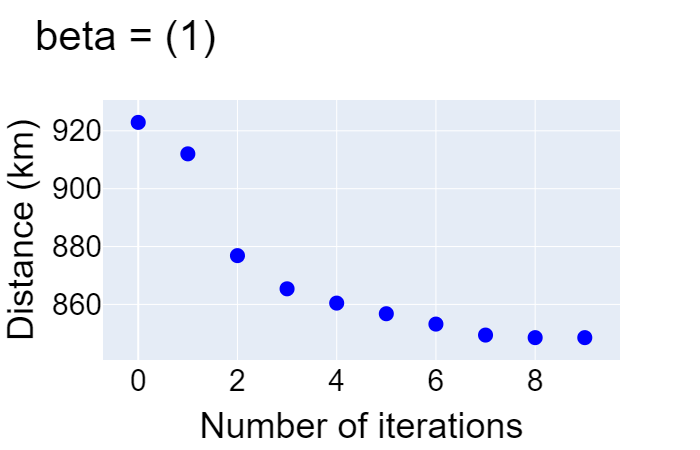
\includegraphics[width=.3\textwidth]{./img/C103_km_newplot (1)}\hfill
	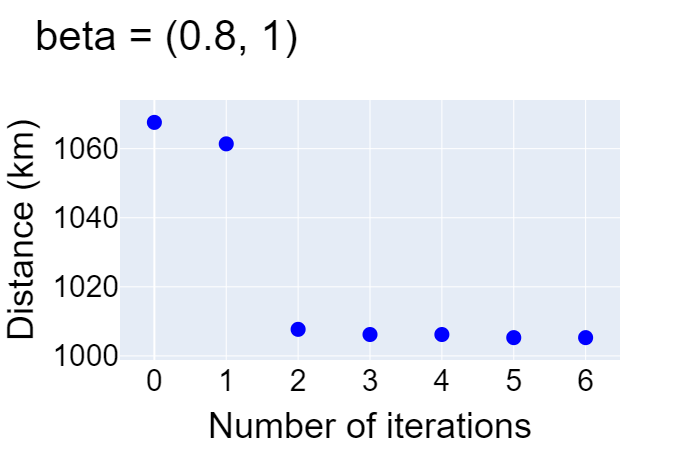
\includegraphics[width=.3\textwidth]{./img/C103_km_newplot (2)}\hfill
	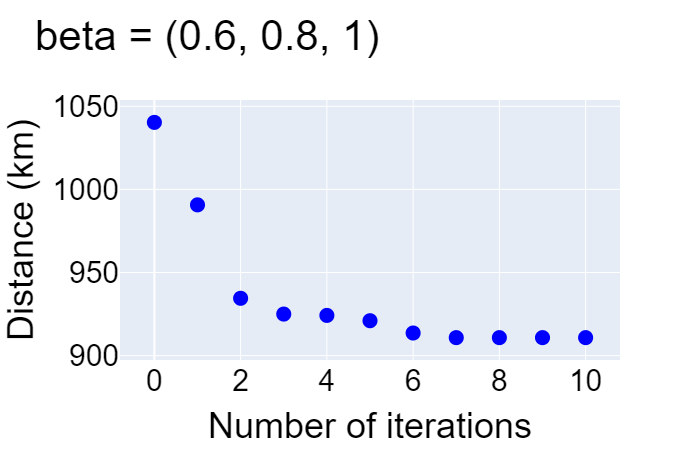
\includegraphics[width=.3\textwidth]{./img/C103_km_newplot (3)}
	\\
	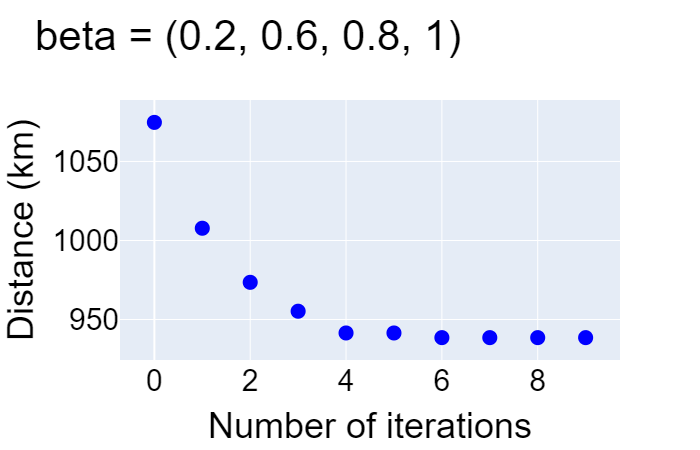
\includegraphics[width=.3\textwidth]{./img/C103_km_newplot (4)}\hfill
	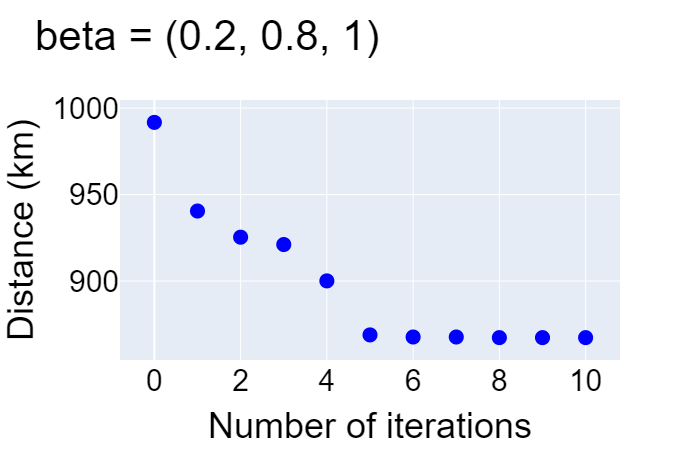
\includegraphics[width=.3\textwidth]{./img/C103_km_newplot (5)}\hfill
	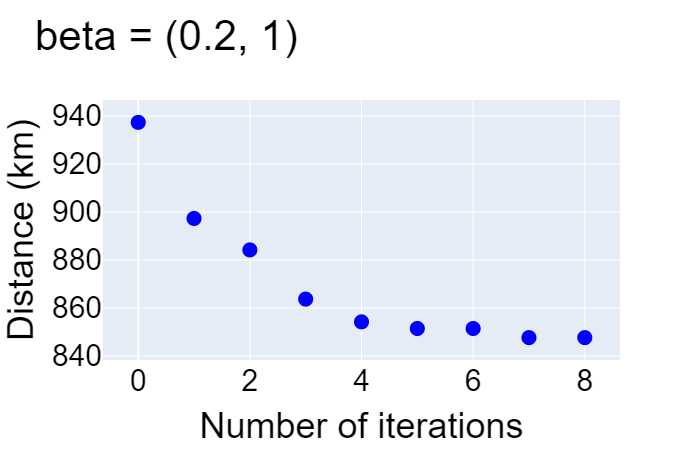
\includegraphics[width=.3\textwidth]{./img/C103_km_newplot (6)}
	\caption{Distance improvement at each iteration of Solomon C103 instance}
	\label{robustedSolomonC103}
\end{figure}

Figure \ref{robustedSolomonC1032} shows the number of routes decrease of the Solomon C103 instance. At most instances, the metaheuristic reaches the minimum number of trucks at first iterations with all $\beta$ values. However, when $\beta = (0.2, 0.6, 0.8, 1)$ the metaheuristc do not reduces the number of routes. Recall that the best results were found with $\beta = (0.2, 0.8, 1)$, when the metaheuristic finds the minimum number of routes at its first iteration.

\begin{figure}[H]
	\centering
	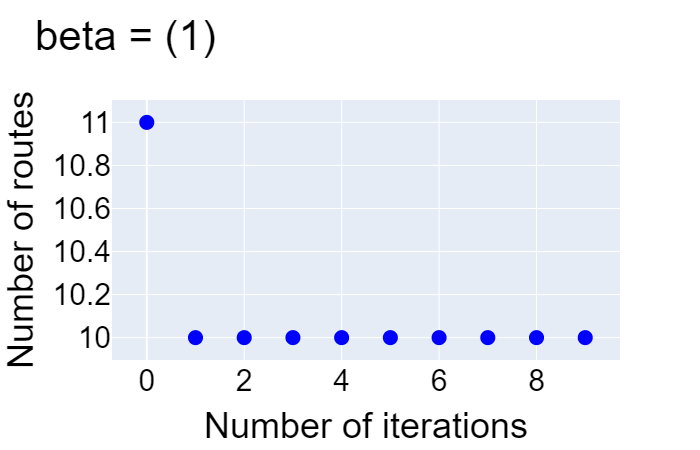
\includegraphics[width=.3\textwidth]{./img/C103_route_newplot (1)}\hfill
	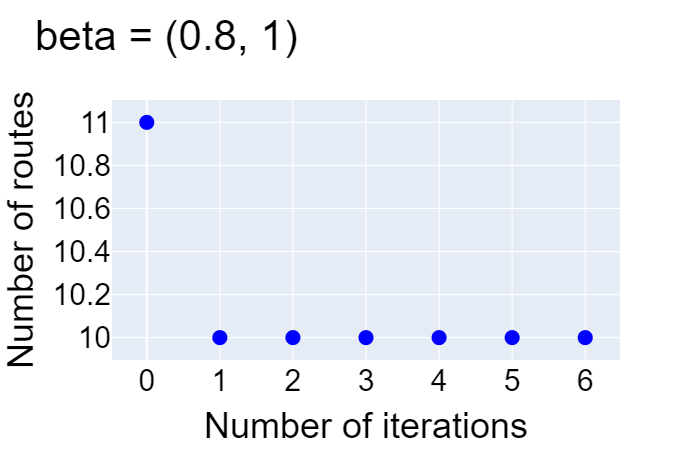
\includegraphics[width=.3\textwidth]{./img/C103_route_newplot (2)}\hfill
	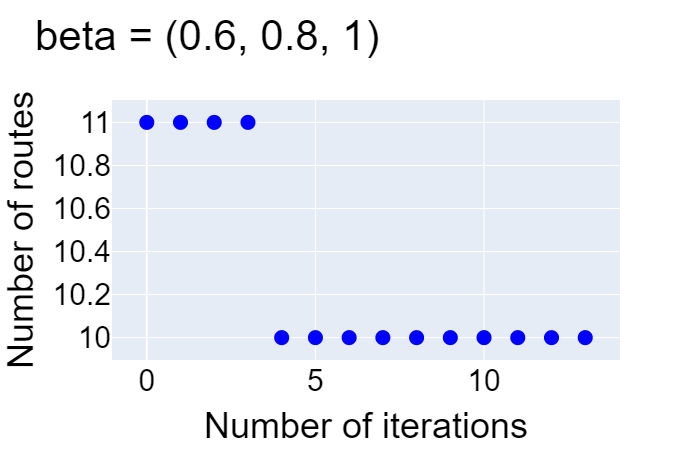
\includegraphics[width=.3\textwidth]{./img/C103_route_newplot (3)}
	\\
	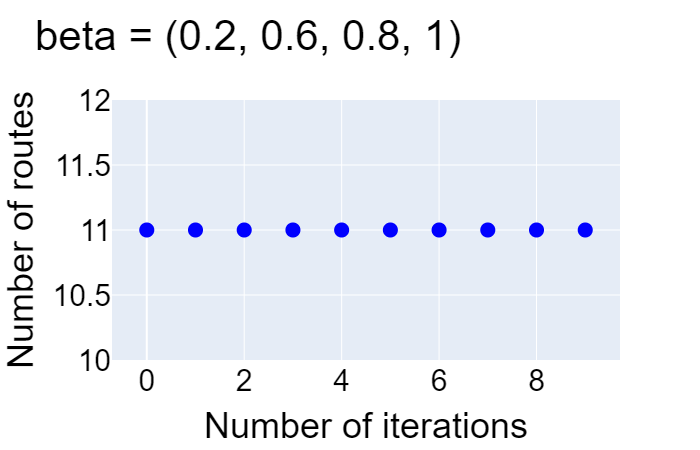
\includegraphics[width=.3\textwidth]{./img/C103_route_newplot (4)}\hfill
	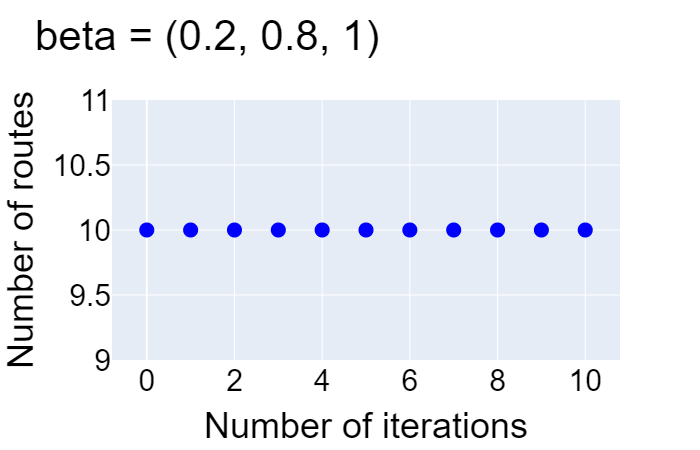
\includegraphics[width=.3\textwidth]{./img/C103_route_newplot (5)}\hfill
	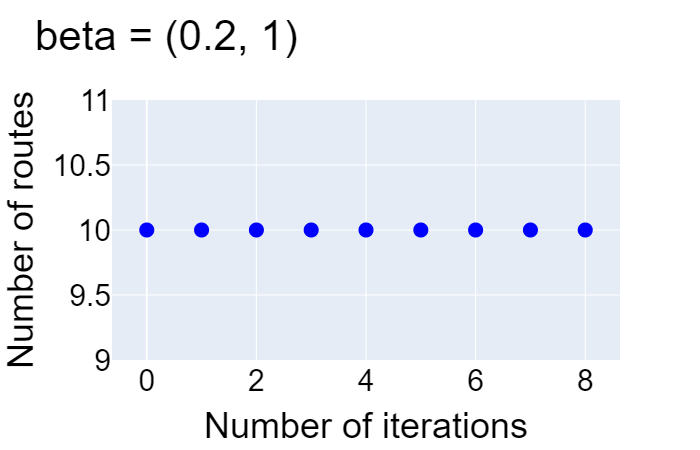
\includegraphics[width=.3\textwidth]{./img/C103_route_newplot (6)}
	\caption{Number of routes improvement at each iteration of Solomon C103 instance}
	\label{robustedSolomonC1032}
\end{figure}



Figure \ref{robustedSolomonC203} shows the distance improvement of the Solomon C203 instance in terms of distance. As the previous example, the metaheuristic performs a big improvement at first iterations with all $\beta$ values. The metaheuristc reach a distance between 1000 and 800 distance units at these first iterations. Finally it makes small improvements until it finishes, finding a minimum distance between 950 and 650. Moreover the number of iteration varies from 6 to 11, which is not a big variation. That implies that the behavior of the metaheuristic is similar in terms of convergence and number of iterations with C103 and C203 instances. It also shows a similar trend with all $\beta$ values

\begin{figure}[H]
	\centering
	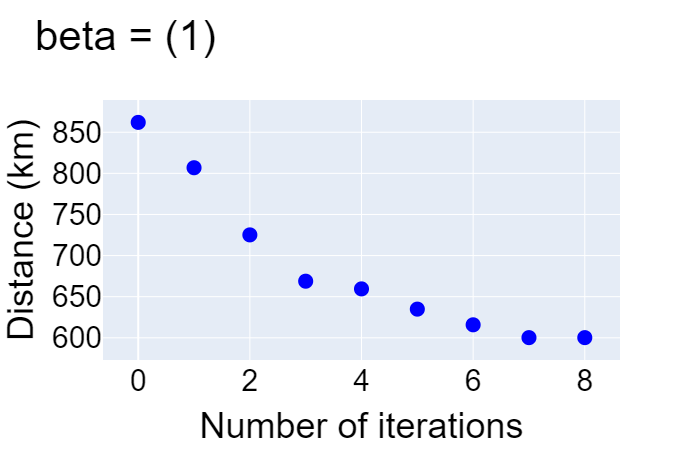
\includegraphics[width=.3\textwidth]{./img/C203_km_newplot (1)}\hfill
	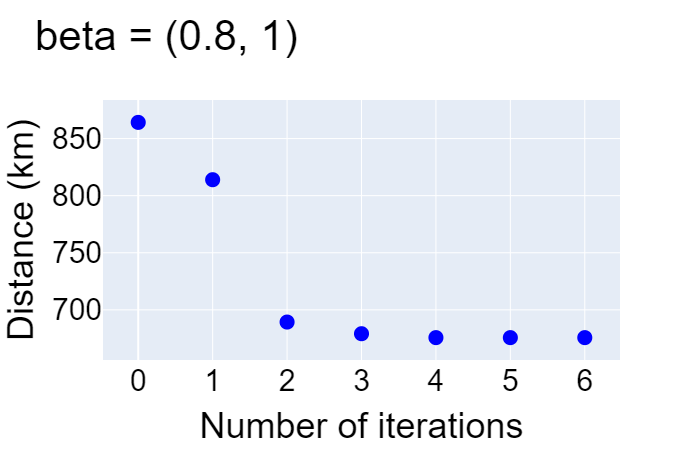
\includegraphics[width=.3\textwidth]{./img/C203_km_newplot (2)}\hfill
	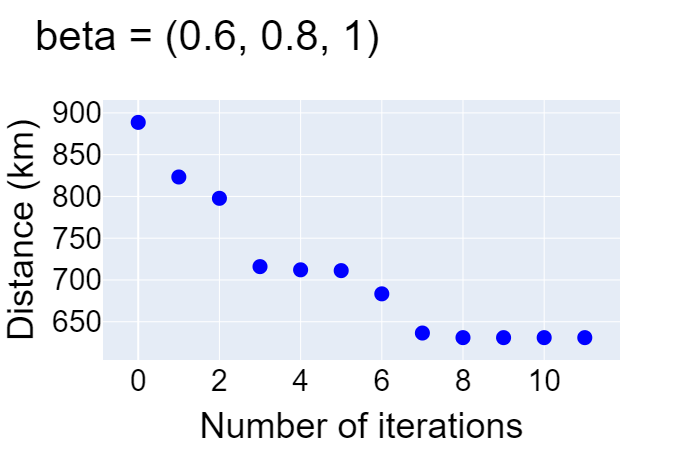
\includegraphics[width=.3\textwidth]{./img/C203_km_newplot (3)}
	\\
	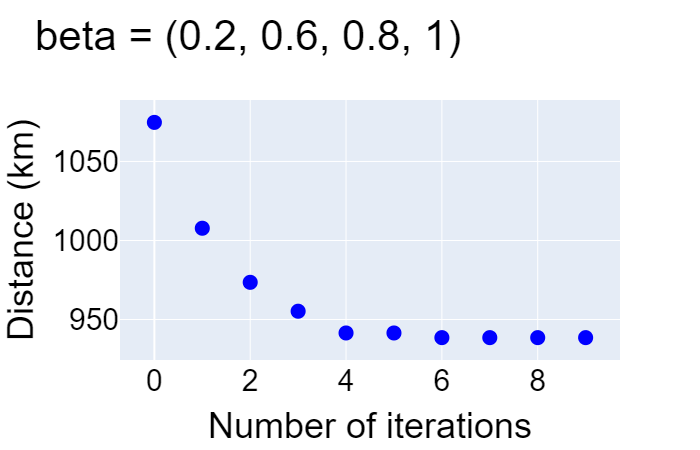
\includegraphics[width=.3\textwidth]{./img/C103_km_newplot (4)}\hfill
	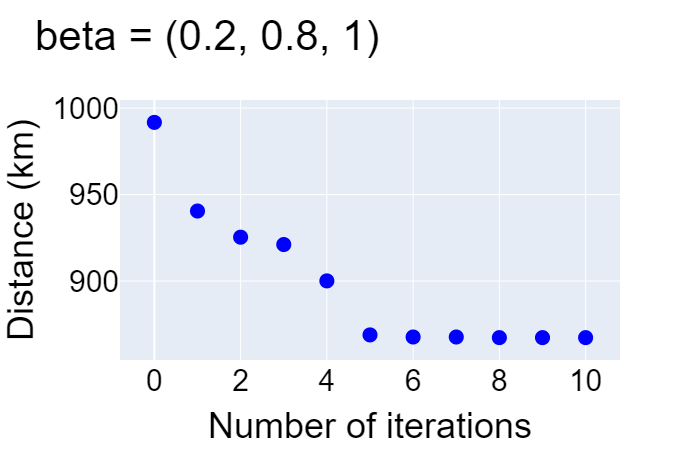
\includegraphics[width=.3\textwidth]{./img/C103_km_newplot (5)}\hfill
	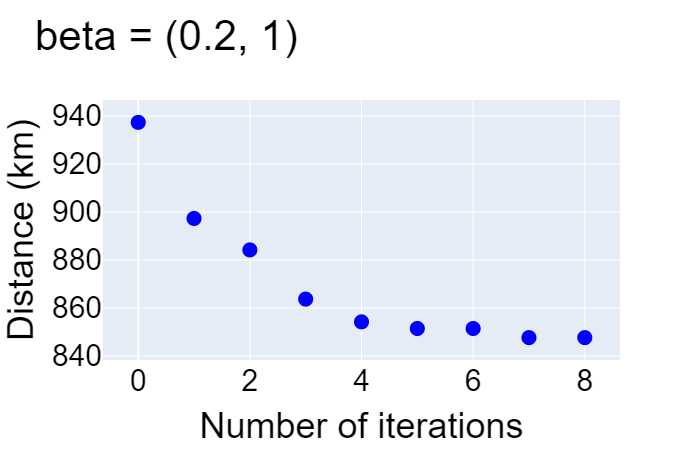
\includegraphics[width=.3\textwidth]{./img/C103_km_newplot (6)}
	\caption{Distance improvement at each iteration of Solomon C103 instance}
	\label{robustedSolomonC203}
\end{figure}

Figure \ref{robustedSolomonC2032} shows the number of routes decrease of the Solomon C203 instance. At most instances, the metaheuristic reaches the minimum number of at first iterations with all $\beta$ values. However, when $\beta = (0.8, 1)$ the metaheuristc do not reduces the number of routes. Recall that the best results were found with $\beta = (0.2, 0.8, 1)$, when the metaheuristic finds the minimum number of routes at its fifth iteration.

\begin{figure}[H]
	\centering
	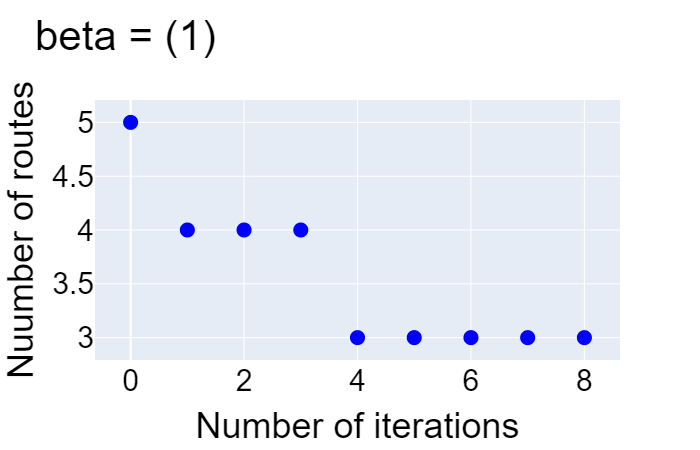
\includegraphics[width=.3\textwidth]{./img/C203_distance_newplot (1)}\hfill
	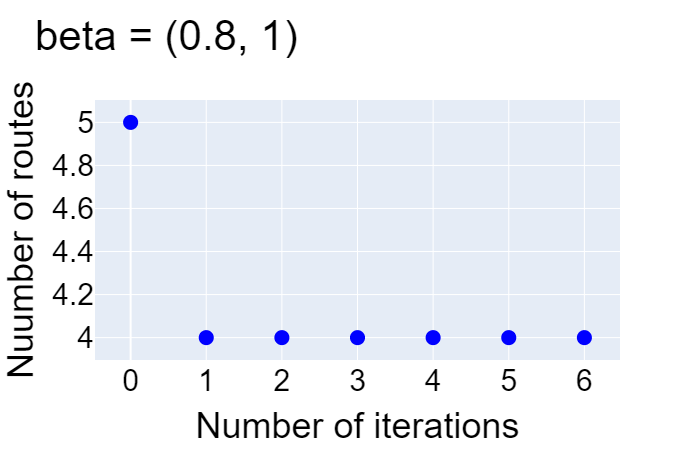
\includegraphics[width=.3\textwidth]{./img/C203_distance_newplot (2)}\hfill
	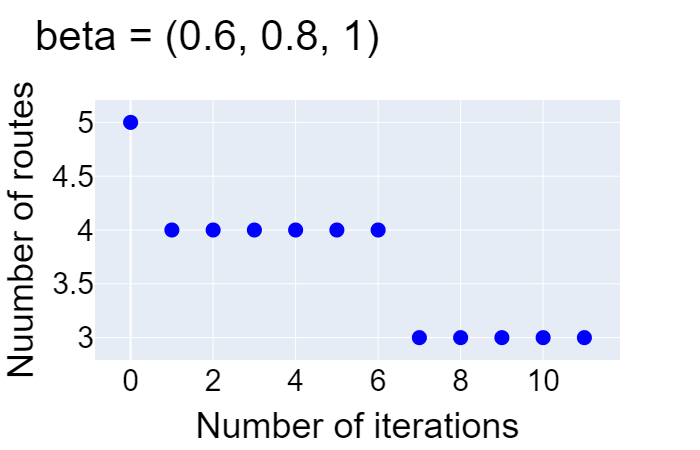
\includegraphics[width=.3\textwidth]{./img/C203_distance_newplot (3)}
	\\
	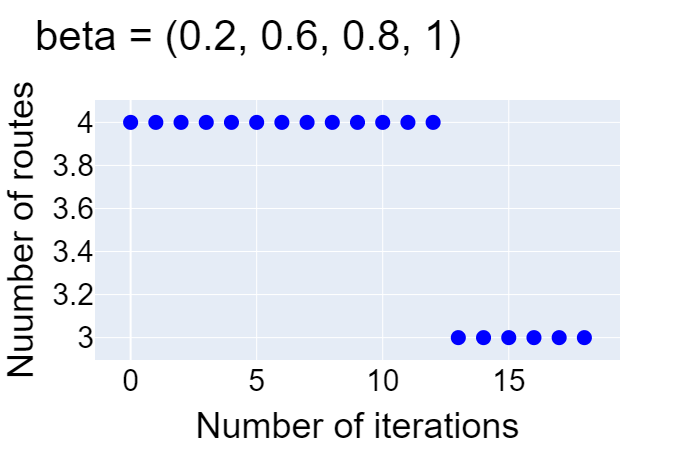
\includegraphics[width=.3\textwidth]{./img/C203_distance_newplot (4)}\hfill
	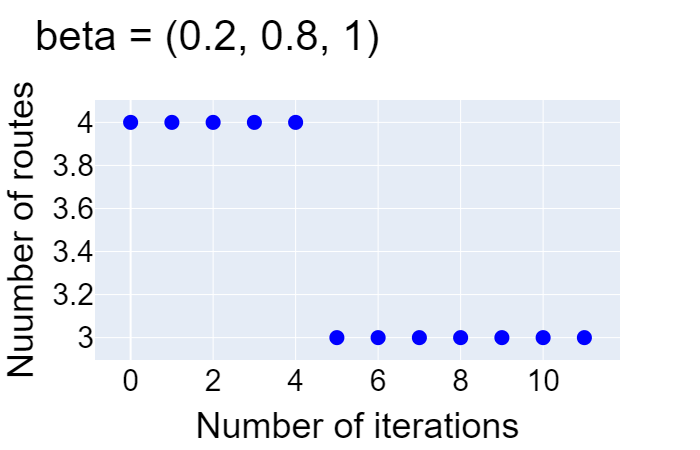
\includegraphics[width=.3\textwidth]{./img/C203_distance_newplot (5)}\hfill
	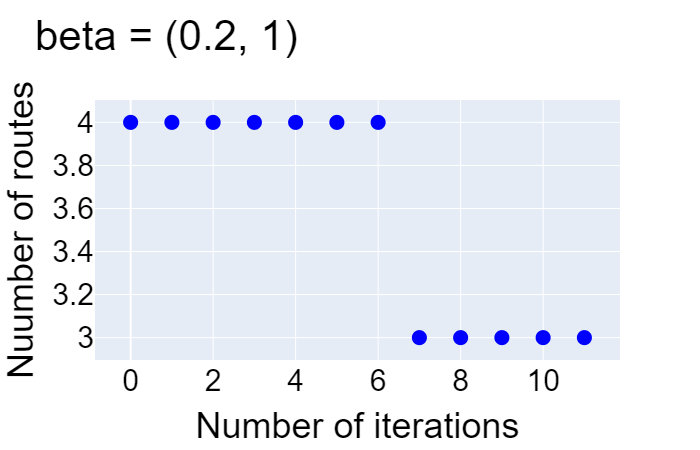
\includegraphics[width=.3\textwidth]{./img/C203_distance_newplot (6)}
	\caption{Number of routes improvement at each iteration of Solomon C103 instance}
	\label{robustedSolomonC2032}
\end{figure}

Finally, figure \ref{robustedAira3} represents how the metaheuristic improves the initial solution at each iteration to 19 farmer instance. s in the previous examples, the metaheuristic performs a big improvement at first iteration under all $\beta$ values. The initial solution has over 700 km and the improved solution at the first iteration has over 500km. Finally the metaheuristic makes small improvements until it finishes. Note that it also has a similar trend at all $\beta$ values.

Results are similar in terms of distance and convergence, that means that the metaheuristic is robust at different $\beta$ values.

\begin{figure}[H]
	\centering
	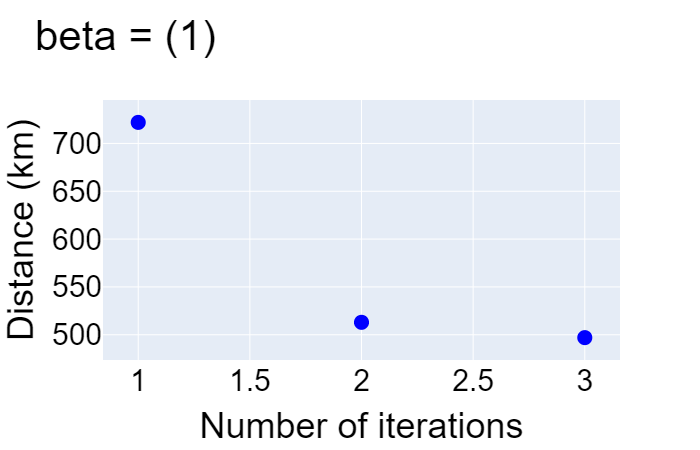
\includegraphics[width=.3\textwidth]{./img/AIRA newplot (1)}\hfill
	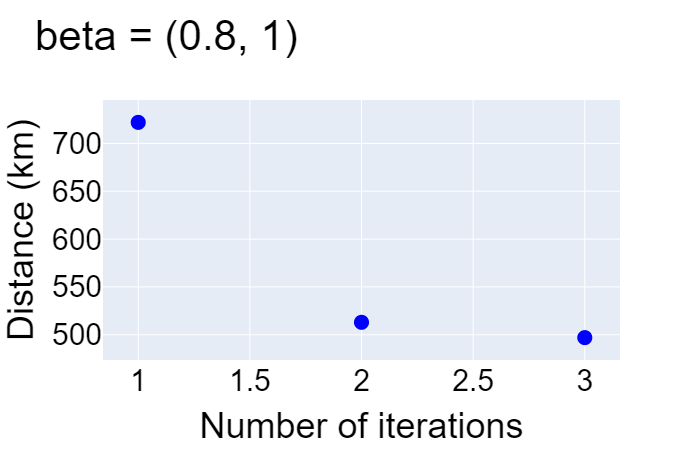
\includegraphics[width=.3\textwidth]{./img/AIRA newplot (2)}\hfill
	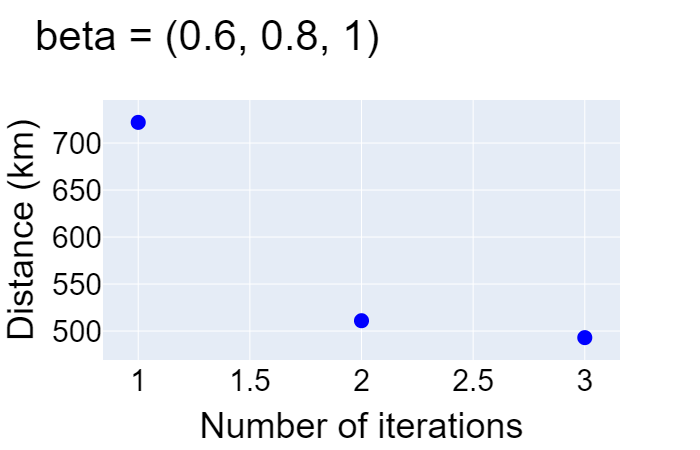
\includegraphics[width=.3\textwidth]{./img/AIRA newplot (3)}
	\\
	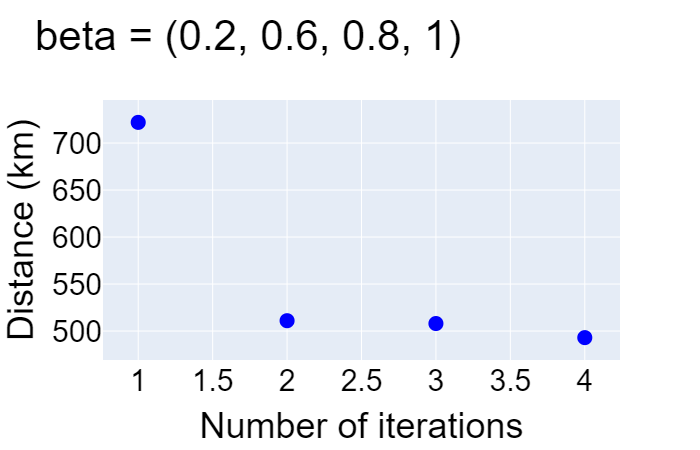
\includegraphics[width=.3\textwidth]{./img/AIRA newplot (4)}\hfill
	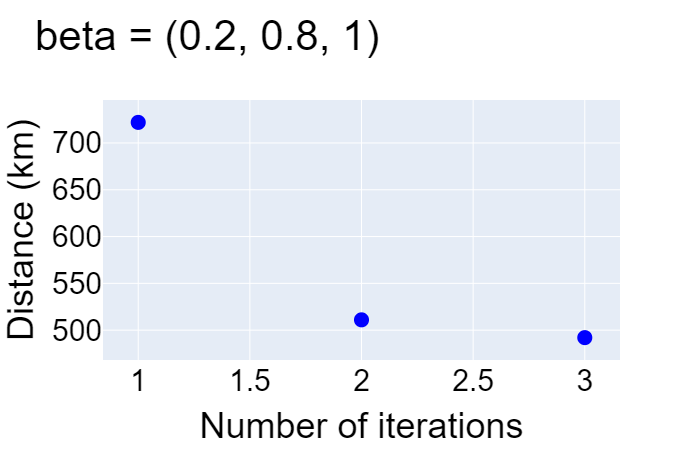
\includegraphics[width=.3\textwidth]{./img/AIRA newplot (5)}\hfill
	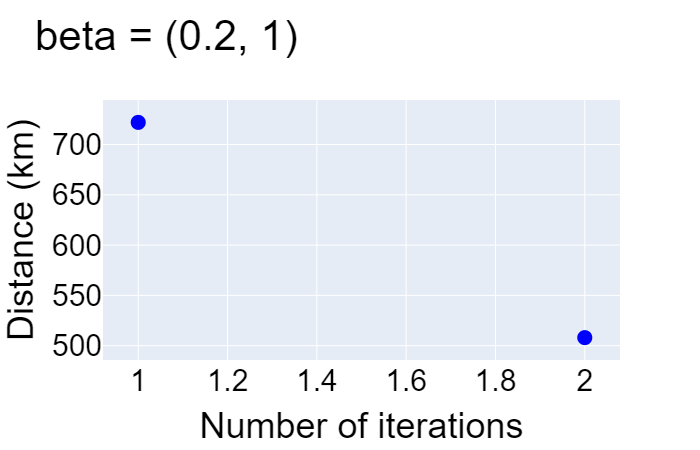
\includegraphics[width=.3\textwidth]{./img/AIRA newplot (6)}
	\caption{Distance improvement at each iteration of 19 farmer instance}
	\label{robustedAira3}
\end{figure}

To sum up, the metaheuristic has proved to perform well on different data sets with the same parameter configuration. By (\cite{Bent}) one can say that the metaheuristic seems to be robust. Furthermore it has similar behavior in terms of number of iterations and convergence.



\chapter{Block II: cooperative game theory}
\label{chap:blockII}
\section{Introducion to game theory}\label{GameTheoryIntro}
In many real situations, if some individuals work together they can improve costs (or benefits) that must be shared among them. Game theory models this situations by cooperative games which are a helpful tool to answer the question ''How to allocate those costs/benefits among the players fairly?''. The cooperative game theory offers a mechanism which allows to distribute expenses in an efficient, fair way and provides incentives for players to cooperate, when it is possible.

The fairly of distribution can be very different depending on the situation of the game i.e., a fairly solution can turn into a unfairly one when circumstances change. Thus many solutions to this problem can be found in the literature. In most cases, the key of fairness is that some players must cooperate, thus players should make an agreement which satisfies to every player of the agreement. Cooperative game theory defines ideal allocation properties which help to find 	
stable solutions.

In game theory, two different games can be defined:
\begin{itemize}
	\item Non-cooperative games, where players compete between them. Each player choose a set of strategies and tries anticipate his rival's strategies to win them.
	\item Cooperative game is a game where two or more players aim the same objective. Players can communicate, negotiate and make agreements in order to get their objectives, i.e., players can transfer their utility with no restriction.
\end{itemize} 

This block gives a review of the main results of the cooperation game theory in section \ref{GameTheoryBackground}. Section \ref{AllocationRules} focus on allocation values such as Shapley value and Aumann-Dr\`eze's value. Section \ref{GameTheoryCooperation} introduces the collaborative routing problem. Finally the section \ref{GameTheoryResults} shows how to allocate cost in such a routing problem.


\section{Game theory background}\label{GameTheoryBackground}

This subsection introduces the main concepts of transferable utility games (TU games).

Let $G^{|N|}$ be the set of all $n-$player games, then an element of $G^{|N|}$ can be represented by a pair $(N,v)$. 


\begin{definition}
	A TU game is given by a pair $(N,v)$, where $N=\{1,2, \dots, n\}$ is the finite set of players which can cooperate and $v:2^{|N|} \rightarrow \mathbb{|N|}$ is the characteristic function. By convention, $v(\emptyset) = 0$.
\end{definition}
The characteristic function can represent savings or cost. This section will introduce some concepts for savings game, i.e., for games whose characteristic function represents benefits. However, this concepts can be defined similarly for cost games.

Deepening the characteristic function, it must be noted that the cost of a player who does not cooperate is noted by $v(i)$, $i \in N$, while the cost of two or more player who cooperate, forming up a coalition $S$, $S \subseteq N$, is noted by $v(S)$ and is called the cost of the coalition $S$. The set of all coalitions among the players in $N$ is noted by $L(N) = \{ S | \forall S \subseteq N, S \ne \emptyset \} $. Observe that the characteristic function assigns a worth $v(S)$, to every coalition $S \subseteq N$.

%\begin{definition}
% A player $i \in N$ is a called a dummy player if for each $S \subseteq N \setminus  \{ i \}$, $v(S \cup \{i\}) - v(S) = v(\{i\})$.
%\end{definition}

Once the characteristic function behavior is known, it could be interesting to define the payoff allocation, which allows to allocate the cost or benefits between players. A payoff allocation is given by a vector $x=(x_{i})_{i \in N}$, $x  \in \mathbb{R}^{|N|}$, where $x_{i}$ is interpreted as the utility payoff to player $i$. Given an allocation $x \in \mathbb{R}^{|N|}$ the following properties must be introduced:
\begin{itemize}
	\item $x$ satisfies efficiency if $\sum_{i = 1}^{|N|} x_{i}   = v(N)$.
	\item $x$ satisfies individually rational if $x_{i} \geq v(i)$, $\forall i \in N$.
	\item $x$ satisfies coalition rational if $\sum_{i \in S}x_{i} \geq v(S)$, $\forall S \subsetneq N$.
\end{itemize}


%\begin{definition}
%An allocation $x$ is said to be feasible for a coalition $S$ the following statements hold:
%\begin{itemize}
%	\item $\sum_{i \in S}x_{i}  = v(S)$
%	\item all players in $S$ can achieve their components of this allocation by dividing among themselves the worth $v(S)$ that they can get by cooperating together.
%\end{itemize}
%, and the 
%\end{definition}

\begin{definition}
	An allocation $x$ is stable for $(N,v)$ if for each $S \subsetneq N $, $\sum_{i \in S} x_{i} \geq v(S)$, i.e., no coalition can improve by not joining to the grand coalition. 
\end{definition}



There exists two different solutions in cooperative game theory: allocations which defines a set of solutions with common characteristics and unique solutions which presents some properties. Some times these unique solutions belongs to a set of solutions. Thus, it knowing if unique solutions belong to a set of solutions is interesting. Let's introduce some concepts which will help with this issue. 

%If an allocation is feasible without reference to any particular coalition, it means that it is feasible for the big coalition $N$.


%A coalition $S$ is said that can be improved on an allocation $x$ if $v(S) > \sum_{i \in S} x_{i}$. That is, $S$ can improve on $x$ if there exists some allocation $y$, such that $y$ is feasible for $S$ and the players in $S$ all get strictly better payoff in $y$ than in $x$.


\begin{definition}
	Given a TU game, $(N,v)$, the set of preimputations for (N,v) is defined by the set of all efficient allocations, i.e.:
	$$I^{*}(N,v) = \{x= (x_i)_{i \in N} \in \mathbb{R}^{|N|}: \sum_{i \in N}x_i = v(N) \}.$$
	
\end{definition}


\begin{definition}
	Given a TU game, $(N,v)$, the set of imputations for (N,v) is defined by the set of all efficient allocations which verifies individually rational, i.e.:
	%An allocation $x \in \mathbb{R}^{|N|}$ is called an imputation for (N,v) if it satisfies:
	$$I(N,v) = \{x= (x_i)_{i \in N} \in I^{*}(N,v) : x_i \geq v({i}),\forall i \in N\}.$$
\end{definition}

%An allocation $x \in \mathbb{R}^{|N|}$ is called an imputation for (N,v) if it satisfies:
%\begin{itemize}
%	\item $x_{i} \geq v(i)$, $\forall i \in N$ (individually rational).
%	\item $\sum_{i = 1}^{|N|} x_{i}   = v(N)$ (efficiency).
%\end{itemize}
One can see that both preimputations and imputations sets have interesting properties but, these sets could be empty for some games. The following property establishes when the imputation set is not empty.

\begin{definition}
	A TU game, $(N,v)$, is called essential if
	$$v(N) \geq \sum_{i=1}^{|N|} v(i)$$
\end{definition}
\begin{proposition}
	A TU game is essential if and only if the set of imputations is not empty:
	$$I(v) \ne \emptyset \iff v(N) \geq \sum_{i=1}^{|N|} v(i).$$
\end{proposition}


%If $v(N) =\sum_{i=1}^{|N|} v(i)$, then $I(N,v)=(v(\{1\}), \dots, v(\{n\}))$. $v(N) > \sum_{i=1}^{|N|} v(i)$ then $I(N,v)$ is an $(n-1)$-dimensional simplex with extreme points $e^{1}, \dots, e^{|N|}$, where $e_{i}^{i}(N,v) = v(N) - \sum_{j \ne i}v_{\{j\}}$. \textbf{edit=1, quizá sobre la última definicion}.

The set of imputations satisfies efficiency and individually rational which are good properties of an allocation. Moreover, coalitional rational is a desirable characteristic for allocation. One of the main concepts of cooperative game theory is the core, which is defined by the set of imputations which satisfy coalitional rational. 

\begin{definition}
	Given a TU game, $(N,v)$, its core is defined by: 
	$$C(N,v) = \{ x \in I(v) : \sum_{i \in S}x_{i}  \geq v(S), \forall S \in 2^{|N|}  \}.$$
\end{definition}
Note that allocations in the core satisfy the minimum requirements that any coalition might demand. Furthermore, the core is the set of imputation that satisfies efficiency, individually rational and coalition rationality. If an allocation is in the core, it will give better payoff to players who cooperate than if they do not cooperate. Moreover, if an allocation is in the core, there is no player who pays less than its marginal total cost, i.e.:
$$ \forall x\in \mathbb{R}^{|N|}, x \in C(N,v) \implies x(S) \geq v(N) - v(N-S) , \hspace{1pt}\forall S \subseteq N .$$

A cost allocation in the core is said to be stable. The class of games with non empty core is the called the class of balanced games.
Moreover, the core is a convex and compact polyhedron in $\mathbb{R}^{|N|}$ whose maximum dimension is $|N|-1$ because it belongs to the hyperplane $\sum_{i=1}^{|N|}x_{i}=v(N)$. However, the core of a game can be empty, thus next concepts will bring an idea of the core.

\begin{proposition}
	If a TU game, $(N,v)$ verifies
	\begin{itemize}
		\item for each $S \subsetneq N$, $v(S) = \sum_{j \in S} v(\{j\})$
		\item $v(N) > \sum_{i \in N} v(\{i\}) $
	\end{itemize}
	then $C(N,v)= I(N,v)$
\end{proposition}

\begin{definition}
	A TU game $(N,v)$ is convex if
	$$v(S \cup \{i\} )- v(S) \leq v(T \cup \{i\} )- v(T), \hspace{1pt}\forall S, T: T \subsetneq S \subseteq N \setminus \{i\}.$$
\end{definition}

The amount $v(S \cup \{i\} )- v(S) $ is called $i's$ marginal contribution to coalition $S$. In convex games, $i's$ marginal contribution to any coalition does not decrease as the coalitions grows. Note that a convex game is balanced, but a balanced game can be no convex.

\begin{proposition}
	The core of a convex game it not empty.
	
\end{proposition}	


%An allocation cost problem is a tuple $(N,v)$ such that $N$ represent the finite set of players and $c:2^N\rightarrow \mathbb{R}$ is a function which assigns to every coalition $S \subsetneq N$ a cost. By convention $c(\emptyset) = 0$. Distributing the cost of the big coalition, $c(N)$, among players is the main aim of this problem. Note that, an allocation cost problem is a TU game which deals with cost instead of profits. 

This subsection ends by introducing the concept of partitional games, where interesting approaches will be considered in this work. 

\begin{definition}
	A TU game with an union system is a tuple $(N,v,P)$ , where $(N,v)$ is a TU game and $P=\{P_{1}, \dots, P_m\}$ is a partition of $N$, which defines the union system.
\end{definition}

Distributing the benefits of the big coalition, $v(N)$, among players in $N$ under the coalitional structure $P$ is the main aim of this games. 

One can see that the main purpose of TU games and partitional games is allocating the worth of $v$. To solve this task allocation rules are introduced in section \ref{AllocationRules}.



\section{Allocation rules}\label{AllocationRules}

Allocation rules indicate how much of the total costs or benefits are assigned to each player. 
In order to ensure that no player pays more than can reasonably be expected of him, the core was
defined. However, the core of a coalitional game may be empty or quite large, which makes the core difficult to apply as a predictive theory. The best that one can hope for would be to derive a theory that finds, for each game in coalitional form, a unique expected payoff allocation for the players. 

There is no single method to select the best allocation rule. For each situation a different cost allocation must be chosen depending on the wishes of the gran-coalition. For example, may some coalitions would choose to minimize the difference in relative cost savings, whereas others may prefer to distribute costs proportional to the stand-alone costs. 

An allocation rule is a function which, returns an allocation $x \in \mathbb{R}^{|N|}$ for each fame $(N,v)$, i.e.:

$$\varphi: \Omega \subseteq G^{|N|}  \rightarrow \mathbb{R}^{|N|} $$
$$ (N,v) \longmapsto \varphi(N,v)$$

Let $(N,v) \in  G^{|N|}$ and $\varphi$ be an allocation rule, then the following properties states:

\begin{itemize}
	\item $\varphi$ is continuous if $\varphi: \mathbb{R}^{2|N|-1} \rightarrow \mathbb{R}^{|N|}$ is continuous.
	\item $\varphi$ is efficient if it returns efficient allocations for all $(N,v)$.
	\item $\varphi$ is individually rational if it returns individually rational allocations for all $(N,v)$.
	\item $\varphi$ is symmetric if for each two players $i,j  \in N$ such that, for each $S \subsetneq N \setminus \{i,j\}$, $v(S \cup \{i\}) - v(S) = v(S \cup \{j\}) - v(S)$ then $\varphi_{i}(N,v) = \varphi_{j}(N,v)$.
	\item  $\varphi$ satisfies the dummy player property if for each $i \in N$ such that for each $S \subsetneq N \setminus \{ i\}$, $v(S\cup \{i\} ) - v(S) = v(\{i\})$ then $\varphi_{ij}(N,v) = v({i})$.
	\item $\varphi$ is scale invariant if for each two games $(N,v)$ , $(N,w)$ and each $r \in \mathbb{R}$ such that, for each $S \subseteq N, w(S)= rv(S)$ then $\varphi(N,w) = r\varphi(N,v)$.
	\item $\varphi$ is translation invariant if for each two games $(N,v)$ , $(N,w)$ and each $\alpha = (\alpha_{1}, \dots, \alpha_{|N|})\in \mathbb{R}^{|N|}$ such that, for each $S \subseteq N, w(S)= v(S) + \sum_{i \in S} \alpha_{i}$ then $\varphi(N,w) = \varphi(N,v) + \alpha$.	
	\item  $\varphi$ satisfies weak coalitional monotony if given two games $(
	N,v)$, $(N,w)$ and $S,T \subsetneq N $ such that $w(T) > v(T)$ and $w(S)= v(S)$, $\forall S \ne T$ then
	$\sum_{i \in T} \varphi_{i}(N,w) \geq \sum_{i \in T} \varphi_{i}(N,v)$.
\end{itemize}

An allocation rule is also called a solution of a TU game. There are many allocation rules in the literature which has very different characteristics. Some may be stable, while others can guarantee unique solutions. As such, one can not just state that any of the cost distributions is ideal. To this end some of the most used cost distributions are introduced. These are the Nucleolus, Shapley value, Aumann-Dr\`eze's value and Equal Profit Method.

Those allocation rules are discussed in the next subsections. Each subsections includes a formal definition of an allocation rule and its properties. 


\subsection{Nucleolus}\label{subNucleolus}

The nucleolus has been introduced by Schmeidler (\cite{Schmeidler}) . The method ensures that the
coalitions with maximum profit retain their profit margins. If the core turns out to be empty,
this can result in some coalitions becoming less profitable.

\begin{definition}	
	For any coalition, $S$, and a given cost allocation, $x$, the excess is defined as follows:
	$e(S,x)=v(S) - \sum_{i \in S}x_{i}$,
	which measures the net transferable worth that $S$ would have left after paying $x_{i}$ to each member $i$.
	%the amount by which coalition $s$ falls short of its potential $v(S)$ in the allocation $x$. Since, the core is defined as the set of imputations such that $\sum_{i \in S}x{i} \geq v(S)$, $\forall S$. 
	%Let $O(x)$ define the vector of excess arranged in decreasing order. 
	
\end{definition}
Note that, $e(S,x) \geq 0$ if and only if coalition $S$ could achieve by itself its share of the allocation $x$. Moreover, $e(\emptyset,x)=e(N,x)=0$.
\begin{definition}
	Let $\leq_{L} \in \mathbb{R}^n$ defines a lexicographical order as follows:
	\begin{itemize}
		\item It can be said that $x <_{L} y$ if there exists $k \in \mathbb{|N|}$, $1 \leq k \leq n$, such that:
		$x_{i} = y_{i}$, $1 \leq k < n$
		$x_k<y_k$
		\item It can be said that $x \leq_{L} y$ if $x=y$ or $x <_{L} y$.
	\end{itemize}
	
	%	For any two allocations $x,y \in \mathbb{R}^N$ and any coalition $S$ one can say that $x$ is strictly preferred to $y$ by all the members of coalition $S$ if $x >_{S} y$ $\iff$ $x_{i} > y_{i}$ $\forall i\ in S$.
	%	Similarly, one can write $x \geq_{S} y$ $\iff$ $x_{i} \geq y_{i}$ $\forall i\ in S$
	
	Given an allocation vector $x \in \mathbb{R}^n$, let $\theta(x)$ be the $2^{|N|}-$tuple whose components are the excess of every coalitions by $x$ ordered by decreasing order, i.e.,
	
	$$\theta_{i(x)} \geq \theta_{j(x)} \text{ if } 1\leq i \leq j \leq 2^{|N|}.$$
\end{definition}

\begin{definition}
	The nucleolus of a TU game $(N,v)$ can be defined as the set:
	$$Nu(N,v) = \{x \in I(N,v) : \theta(x) \leq_{L} \theta (y), \forall y \in I(N,v) \}.$$
\end{definition}

An imputation $x$ is in the core if an only if all its excess are negative or zero. Thus the excess vectors of allocations in the core are lexicographical smaller that any allocation which is not in the core. That implies, that if the core of a TU game is not empty then the nucleolus is in the core. 

Note that the nucleolus can be formed up by more than one point. The following results are useful to determine the points of the nucleolus.


\begin{theorem}
	The nucleolus satisfies dummy player, symmetric player, weak coalitional monotony properties and it is scale and translation invariant.
\end{theorem}



\subsection{The Shapley Value}\label{subShapley}

Shapley (\cite{Shapley}) approached the solution of a TU game axiomatically. That is, he asked that kinds of properties might be expected such a solution concept to satisfy. Shapley characterized the mappings $\Phi$, that satisfy these properties. A permutation of the set of players $N$ is any function $\pi : N \rightarrow N$ such that, for every $j \in N$, there exists exactly one $i \in N$ such that $\pi(i)=j$. Given any such permutation $\pi$ and any coalitional game $v$, let $\pi v$ be the coalitional game such that $\pi v ( \{\pi(i) | i \in S \}) = v (S),$ $\forall S \subseteq N$. That is the role of any player $i$ in $v$ is essentially the same as the role of the player $\pi (i)$ in $\pi v$. Shapley's first axiom asserts that only the role of a player on the game should matter, not his specific names or label in the set N.

\begin{axiom}
	(Symmetry). For any $ v \in \mathbb{R}^{L(N)}$, any permutation $\pi: N \rightarrow N$ and any player $i \in N$, $\Phi_{\pi(i)} = \Phi_{i}(v)$.
\end{axiom}

A coalition is called a carries of a coalitional game $v$ if $v( S \cup R) = v(S) $, $\forall S \subseteq N$.
If $R$ is a carries of $v$, them all players who are not in $R$ are called dummies in $v$, because their entry into any coalition cannot change its worth. The second axiom asserts that the players in a carrier set should divide their joint worth among themselves, allocating nothing to the dummy players.

\begin{axiom}
	(Carrier). For any $ v \in \mathbb{R}^{L(N)}$ and any coalition $R$, if $R$ is a carrier of $v$ then $\sum_{i \in R}\Phi_{i}(v)= v(R)$.
\end{axiom}


\begin{axiom}
	(Additivity). For all game $(N,v) $ and $(N,w)$, then $\Phi(N, v+w) = \Phi(N, v) + \Phi(N, w) $.
\end{axiom}

Observe that Shapley showed that there is a unique mapping $\Phi$, called the Shapley value, that satisfies these three axioms.

\begin{theorem}
	\label{thShapley}
	There is exactly one function $\Phi: \mathbb{R}^{L(N)} \rightarrow \mathbb{R}^{|N|}$, that satisfies axioms 3.1, 3.2 and 3.3. This function satisfies the following equation, for every $i \in N$ and every $v \in \mathbb{R}^{L}$. This rule is called Shapley value and can be computed by:
	$$ \Phi_{i}(v) = \sum_{S \subseteq N - i }\frac{|S|!(|N|-|S|-1)!}{|N|!} (v(S \cup \{i\}) - v(S)).$$ 
\end{theorem}

One can find the Shapley value by the formula given in theorem \ref{thShapley} but an alternative expression can be found in the literature. Let's suppose that players are in the big coalition under some order $R = i_1,i_2, \dots, i_n$. Under this order the $i's$ marginal contribution, where $i = i_k$ can be defined by:
$$\gamma_i(R) = v(i_1,i_2, \dots, i_k) - v(i_1,i_2, \dots, i_{k-1})$$
An equivalent expression can be found computing $\gamma_i(R)$ for all permutations of $R$.
\begin{theorem}\label{ShapleyConvexo}
	Let $(N,v)$ be a TU game, the Shapley value of the game is in its core if and only if the game is convex. 
\end{theorem}

Finding the Shapley value involves lots of computations, because the $i's$ marginal contribution must be calculate for every player and for any coalition. Thus calculating this value for large problems can involve lot of time of computation. Nevertheless, Aumann and Dr\`eze gave an interesting approach to this problem. Subsection \ref{subAumann} provides a review of their allocation rule.

\subsection{Aumann-Dr\`eze's value}\label{subAumann}

Aumann and Dr\`eze, (\cite{Aumann}) considered that for a TU partitional game, once a partition $\{P_1,\dots,P_m\}$ of $N$ is made, then $m$ independent cooperation problems can be studied, thus they use Shapley value to assigns the cost of every union $P_k$ among its players. 

In order to introduce the main results to characterize Aumann-Dr\`eze's value, let $G(N)$ be the vectorial space of characteristic functions over $N$. 

\begin{definition}
	A partitional value over $G(N)$ is a function $\phi$,
	
	$$\phi:G(N) \times P(N) \rightarrow \mathbb{R}^{|N|} $$
	
	which verifies local efficiency, i.e.:
	
	$$\sum_{i \in P_K}\phi_{i}(N,v,P)=v(P_k) \text{, }\forall v \in G(N) \text{, } P \in P(N) \text{, } P_k \in P.$$	
\end{definition}

Let $\phi$ be a partitional value, then the following properties states:
\begin{itemize}
	\item $\phi$ satisfies the dummy player property if $\forall v \in G(N)$, $P\in P(N)$, $\forall i \in N$, where $i$ is a dummy player in $v$, then $\phi_i(N,v,P)=0$.
	\item $\phi$ satisfies anonymity with unions property if $\forall v \in G(N)$, $P\in P(N)$, for every permutation $ \pi v$, where $P$ is invariant, then
	$\sum_{i \in S}\phi_{i}(N,\pi v, P)= \sum_{i \in S} \phi_{\pi (i)}(N,v,P)$ $\forall S \subsetneq N$, where $\pi v(S)= v( \{ \pi (i): i \in S\})$.
	\item $\phi$ satisfies the additivity property if $\forall v,w \in G(N)$, $P\in P(N)$, then 
	$\phi(N,v+w, P) = \phi(N,v,P) + \phi(N,w,P)$.
	\item $\phi$ satisfies the symmetry with unions property if $\forall v \in G(N)$, $P\in P(N)$, $\forall i,j \in N$, $i \ne j$, $i,j$ symmetric in $v$ and $P_{i} = P_{j}$, then 
	$\phi(N,v,P) = \phi_{j} (N,v,P)$.
	\item $\phi$ satisfies the balanced contributions with unions property if $\forall v \in G(N)$, $P\in P(N)$ and $\forall i,j \in N$, such that $P_i = P_j$, then
	
	$\phi_{i}(N,v,P) - \phi_{i}(N,v,P^{-j}) = \phi_{j}(N,v,P) - \phi_{j}(N,v,P^{-i})$, 
	
	where for each $k \in N$,
	$P^{-k}=\{ P_{(k)}  \setminus \{k\}, \{k\} \} \cup \{P_{i} : P_{i} \in P, P_{i} \ne P_{(k)} \}  $.
\end{itemize}

Note that balanced contributions with unions property implies that the cost of player $i$ when the player $j$ leaves their common union to form a class form by itself, is the same cost of the player $j$ when $i$ leaves the union. 
\begin{definition}\label{AD=Sahpley}
	
	A partitional Shapley value over $G(N)$ is a partitional value $\phi \in G(N)$ such that:
	
	$$\phi(N,v,P^N) = \Phi(N,v) \text{, } \forall v \in G(N)$$
\end{definition}


\begin{definition}
	
	The Aumann-Dr\`eze value is the partitional Shapley value $\alpha$ over $G(N)$:
	
	$$\alpha_i (N,v,P) = \Phi_{i}(P_i, v_{p_{i}}) \text{, } \forall v \in G(N) \text{, } P \in P(N) \text{, } i \in N,$$
	
	where $P_{i}$ denotes the union, or class, of $P$ where player $i$ belongs to and $v_{P_{i}}$ denotes the constraint of the game $v$ to $P_i$.
\end{definition}

\begin{theorem}
	The Aumann-Dr\`eze value, $\alpha$, is the unique partitional value over $G(N)$ that satisfies dummy player, anonymity with unions and efficiency properties.
\end{theorem}

\subsection{Equal Profit Method}

The Equal Profit Method (EPM) has been introduced by Frisk et al. (\cite{Frisk}). They found out companies may not like cost allocations differences between companies. It turned out that companies did not understand why some coalition members would receive higher relative savings in comparison to others. To solve that situation they designed a method to maximize the acceptance, that is, to to minimize the maximum difference between the allocations relative to stand-alone costs of each customer. The allocation is determined using the following linear programming problem:

\begin{equation}\label{eq1}
\begin{split}
\textrm{Objective min } f
\end{split}
\end{equation}
$\textrm{subject to}$

\begin{equation}\label{eq2}
\begin{split}
\frac{x_i}{c(\{i\})} - \frac{x_j}{c(\{j\})} \leq f \textrm{ } \textrm{ } \forall i,j \in N,\textrm{ } i!=j
\end{split}
\end{equation}

\begin{equation}\label{eq3}
\begin{split}
\sum_{i \in S} x_i \leq c(S)\textrm{ }\textrm{ } \forall S \subseteq N
\end{split}
\end{equation}

\begin{equation}\label{eq4}
\sum_{i \in N} x_i  = c(N)
\end{equation}

\begin{equation}\label{eq5}
x_i \in \mathbb{R}^{+} \textrm{ } \forall i \in N
\end{equation}

\begin{equation}\label{eq6}
f \in \mathbb{R}^{+} 
\end{equation}

where $f$ denotes the maximum relative difference in the cost allocation and $x_i$ denotes the allocation cost of player $i$. Constraint \ref{eq2} enforce to minimize the relative difference of cost allocation. Constraint \ref{eq3} and \ref{eq4} ensure that the allocation is in the core. That implies that the lineal problem is infeasible if the core is empty, thus the EPM can not be computed whether the core is empty. Finally constraints \ref{eq2} holds $\frac{x_i}{c(\{i\})} - \frac{x_j}{c(\{j\})} \leq f$ and $\frac{x_j}{c(\{j\})} - \frac{x_i}{c(\{i\})} \leq f$ for all players $i$ and $j$. Hence, the allocation may not be unique, as one could potentially determine alternate allocated values for players $i$ and $j$.


\subsection{Lorenz allocation}
The Lorenz allocation has been introduced by Arin (\cite{Arin}). This allocation tries to minimize
the smallest difference between the absolute allocations rather than the relative difference as
the EPM does. The Lorenz method can be represented by the following linear programming
problem:
\begin{equation}\label{eq11}
\begin{split}
\textrm{Objective min } f
\end{split}
\end{equation}
$\textrm{subject to}$

\begin{equation}\label{eq22}
\begin{split}
x_i - x_j \leq f \textrm{ } \textrm{ } \forall i,j \in N,\textrm{ } i!=j
\end{split}
\end{equation}

\begin{equation}\label{eq33}
\begin{split}
\sum_{i \in S} x_i \leq c(S)\textrm{ }\textrm{ } \forall S \subseteq N
\end{split}
\end{equation}

\begin{equation}\label{eq44}
\sum_{i \in N} x_i  = c(N)
\end{equation}

\begin{equation}\label{eq55}
x_i \in \mathbb{R}^{+} \textrm{ } \forall i \in N
\end{equation}

\begin{equation}\label{eq66}
f \in \mathbb{R}^{+} 
\end{equation}

where $f$ denotes the maximum relative difference in the cost allocation and $x_i$ denotes the allocation cost of player $i$. 
Constraint \ref{eq22} enforce to minimize the relative difference of cost allocation. Constraint \ref{eq33} and \ref{eq44} ensure that the allocation is in the core. As mention in previous section, that implies that the lineal problem is infeasible if the core is empty, thus the Lorenz allocation can not be computed whether the core is empty. Moreover, by constraint \ref{eq22} the allocation may not be unique, as one could potentially determine alternate allocated values for players $i$ and $j$.
Note that both Equal Profit Method and Lorenz are not unique if the lineal problem has multiple solutions.

\section{Cooperation in VRP}\label{GameTheoryCooperation}

Transport problems model many companies situations. Frequently, different companies have to visit the same customers or their customers are closed to each other. Companies can cooperate by visiting their customers together to reduce their transport cost.

Collaborative vehicle routing may refers to all kinds of cooperation, which are intended to increase the efficiency of vehicle fleet operations (\cite{Gansterer}). The transportation is one of the main contributors of $CO_2$ emissions, (\cite{Ballot}), in this line increasing efficiency may serve to ecological goals. Some public authorities are encouraging companies to collaborate, because collaborative vehicle routing has side effects such as reduced road congestion, and noise pollution. Thus, it is not surprising that collaborative vehicle routing is an active research area of high practical importance.
r
The collaborative routing problem raises a main question: how to split the benefit among the companies. This thesis reviews cost allocation methods as a tool for allocating costs in the collaborative routing problem. Cost allocation methods splits the common cost among the participants. The most simple solution to cost allocation is splitting the common cost equally, weighted by any criteria. However, this cost allocation is probably unfair, for example, maybe its allocates a company more cost than when operating alone. 

Most problems in collaborative transportation use sharing methods based on cooperative game theory. The authors found over forty different methods, which can be categorized as traditional or ad hoc concepts. They show that in the huge majority of studies, one of the following three methods is used:
\begin{itemize}
	\item the Shapley value, \ref{subShapley}, which is generally the
	most applied method (e.g. \cite{Kimms}).
	\item proportional methods (e.g. \cite{Frisk}).
	\item the nucleolus, \ref{subNucleolus}. (e.g. \cite{Agarwal}).
\end{itemize}

Moreover, there are some papers which faces the cost allocation using methods such as Equal Profit Method (\cite{Frisk}) and the Lorenz allocation rule (\cite{Zon}).

As disused in previous section, a well known allocation rule for small cooperative games is the Shapley value. When the data set to be faced is quite big, computing this value involves lots of calculus and computing time. However, the Aumann-Dr\`eze value is a good alternative to allocate the cooperative cost. To compute this value one can consider a partitional game whose partitions are induced by the routes of a routing configuration, and compute the Shapley value for each of these partitions. To reduce computation memory, the partitional approach can be also used to compute the Equal Profit Method and the Lorenz allocation rule.

In the literature one can find two different approaches to the collaborative routing problem (\cite{Gansterer}):
\begin{itemize}
	\item Articles that focus on the transportation problems, while cost allocation is not taken
	into account.
	\item Articles dealing with cost allocation, while the transportation problem is neglected.
\end{itemize}	

For experimental results, this thesis follows the second approach. For experimental results, it considered a transportation problem solved in the previous section \ref{results}, and it focus on how to allocate its costs.

The Aumann-Dr\`eze value, the Equal Profit Method and the Lorenz rule were selected to tested. Section \ref{CooperationAIRA} shows small example, where the Shaplay value is not stable and both the Equal Profit Method and the Lorenz rule have no a feasible solution. Section \ref{CooperationSolomon} faces a large routing problem, of hundred customers, and discuss the differences between each allocation rule.

%This work considers the data sets solved in \ref{chap:blockI} to allocate transport costs between customers. A well known allocation rule for small games is the Shapley value. However the data sets to be faced are quite big, which defines a large cooperative game. Thus computing this value involves lots of calculus and computing time. However, the Aumann-Dr\`eze value is a good alternative to allocate the cooperative cost. To compute this value one can consider a partitional game whose partitions are induced by the routes of a routing configuration. As discuses \ref{AD=Sahpley}, the Aumann-Dr\`eze value can be found by computing the Shapley value of each route. 

%This section shows how allocation rules distribute costs of problems faced in section \ref{results}: the agricultural cooperative's problem and the Solomon benchmark.

\subsection{Experimental results}\label{GameTheoryResults}

These section applies the allocation rules introduced in section \ref{AllocationRules}. To perform this task some code was develop in Python. That code computes the Aumann-Dr\`eze's value by computing the Shapley value of each route of a given solution. Furthermore, the code can also compute the Equal Profit Method and the Lorenz value. Library \href{https://pypi.org/project/PuLP/}{PuLP} was used to model the lineal programming problem and CBC solver was used to solve the problem.

\subsubsection{Agricultural cooperative}\label{CooperationAIRA}


The cooperative is formed by farmers which may have to pay the travel costs. Thus travel costs must be allocated among farmers. The cooperative its formed by 1500 farmers, which defines a large cooperative game. Thus transportation cost is allocated by the Aumann-Dr\`eze value.

To illustrate this computation a route of the routing configuration computed in section \ref{results-AIRA} was selected. In this example the number of customers of one route ranges from 1 to 3 customers, what defines small cooperative game. Let's select one route from the computed solutions. It starts from the depot visits the customers 8, 7, 6 and it ends at the depot. Table \ref{VarthetaCooperative} provides transport cost for each coalition while table \ref{ShapleyCooperative} shows the computation of the Shapley value.


\begin{table}[H]
	\centering
	\begin{tabular}{c|c|c|c}
		%	\hline 
		$S$ & $v(S)$ & $S$ & $v(S)$ \\ 
		\hline 
		$\{\emptyset\}$ & 0 & $\{8,7\}$ & 755.33 \\ 
		\hline 
		$\{8\}$ & 272.72 & $\{8,6\}$ & 593.44 \\ 
		\hline 
		$\{7\}$ & 463.63 & $\{7,6\}$ & 773.89 \\ 
		\hline 
		$\{6\}$ & 289.72 & $\{8,7,6\}$ & 1079.06 \\ 
		%	\hline
	\end{tabular} 
	\caption{ Characteristic function}
	\label{VarthetaCooperative}
\end{table}


\begin{table}[H]
	\centering
	
	\scalebox{0.9}{
		\begin{tabular}{c|c|c|c}
			%	\hline 
			$R$ & 1 & 2 & 3 \\ 
			\hline 
			876 & $v(8) - v(\emptyset) = 272.27$ & $v(8,7) - v(8) = 483.06$ & $v(8,7,6) - v(8,7) = 323.72$ \\ 
			\hline 
			867 & $v(8) - v(\emptyset) = 272.27$ & $v(8,7,6) - v(8,6) = 485.61$ & $v(8,6) - v(8) = 321.18$ \\ 
			\hline 
			786 & $v(8,7) - v(7) = 291.7$ & $v(7) - v(\emptyset) = 463.63$ & $v(8,7,6) - v(8,7) = 323.73$ \\ 
			\hline 
			768 & $v(8,7,6) - v(7,6) = 305.17$ & $v(7) - v(\emptyset) =  463.63$ & $v(7,6) - v(6) = 310.25$ \\ 
			\hline 
			687 & $v(8,6) - v(6) = 303.72$ & $v(8,7,6) - v(8,6) = 485.61$ & $v(6) - v(\emptyset) = 289.72$ \\ 
			\hline 
			678 & $v(8,7,6) - v(7,6) = 305.17$ & $v(7,6) - v(6) = 484.16$ & $v(6) - v(\emptyset) =  289.72$ \\ 
			\hline 
			$sum$ & $1750.31$  &  $2865.72$ &  $1858.33$  \\ 
			%	\hline 
		\end{tabular} 
	}
	\caption{Calculus of the Shapley value}
	\label{ShapleyCooperative}
\end{table}

Finally, the Shapley value of this game is $\Phi = (\sfrac{1750.31}{3!},\sfrac{2865.72}{3!}, \sfrac{1858.33}{3!})$. A desirable characteristic of allocations is the stability. Remember that an allocation vector is stable if it belongs to the core. By theorem \ref{ShapleyConvexo}, proving whether this game is convex is enough to assets if the Shapley value is in the core. Let $i = 8$, $S=\{7,6\}$ and $T = \{7\}$ then $v(S \cup \{i\} )- v(S) \nleq v(T \cup \{i\} )- v(T)$, because $v(N) -v(7,6) \nleq v(8,7)-v(7)$, since $301.17 \nleq 291.8$. 

Hence this game is not convex and the Shapley value is not stable because it does not belong to the core. Moreover, the EPM and the Lorenz allocation models were executed to these values, but the lineal programming problem which represents this problem is infeasible.

\subsection{Solomon benchmark}\label{CooperationSolomon}

Figure out that the travel cost of the Solomon benchmark must be allocated among its customers. These data set is formed by 100 customers, which defines a large cooperative game. Thus the Aumann-Dr\`eze's value is introduced to distribute transport cost.

To illustrate this computation let's randomly consider one instance of the Solomon benchmark, for example the data set RC105. Let's consider the best known solution published at this \href{https://www.sintef.no/projectweb/top/vrptw/solomon-benchmark/100-customers/}{link}, which has 10 routes and 1629.44 distance units. Figure out that one distance unit costs one money unit, in this way 1629.44 money units must be splited among 100 customers. The solution has the following routes:

\begin{table}[H]
	\centering
	\begin{tabular}{c| c |c |c}
		\hline 
		%	\centering		
		P	&	Route & Cost & N\textordmasculine of customers	\\
		\hline
		1  & (0, 90, 53, 66, 56, 0) & 73.45 & 4 \\
		2  & (0, 63, 62, 67, 84, 51, 85, 91, 0) & 129.29 & 7 \\
		3  & (0, 72, 71, 81, 41, 54, 96, 94, 93, 0) & 127.54 & 8 \\
		4  & (0, 65, 82, 12, 11, 87, 59, 97, 75, 58, 0) & 142.51 & 9 \\
		5  & (0, 33, 76, 89, 48, 21, 25, 24, 0) & 167.05 & 7 \\
		6  & (0, 98, 14, 47, 15, 16, 9, 10, 13, 17, 0) & 121.02 & 9 \\
		7  & (0, 42, 61, 8, 6, 46, 4, 3, 1, 100, 0) & 144.53 & 9 \\
		8  & (0, 39, 36, 44, 38, 40, 37, 35, 43, 70, 0) & 132.93 & 9 \\
		9  & (0, 83, 19, 23, 18, 22, 49, 20, 77, 0) & 143.05 & 8 \\
		10 & (0, 31, 29, 27, 30, 28, 26, 32, 34, 50, 80, 0) & 134.62 & 10 \\
		11 & (0, 92, 95, 64, 99, 52, 86, 57, 74, 0) & 122.76 & 8 \\
		12 & (0, 69, 88, 78, 73, 60, 0) & 81.7 & 5 \\
		13 & (0, 2, 45, 5, 7, 79, 55, 68, 0) & 108.97 & 7 \\
		\hline 
	\end{tabular} \
	\caption{Best known solution for Solomon RC105 instance}
	\label{routes}
\end{table}\


Let's consider a partitional game whose partitions are induced by each route of these solution. Thus the Aumann-Dr\`eze's value, $\alpha$, can be computed by the Shapley value of each route, that is:

$$\alpha_i (N,v,P) = \Phi_{i}(P_i, v_{p_{i}}) \text{, } \forall v \in G(N) \text{, } P \in P(N) \text{, } i \in N,$$
where $P_{i}$ denotes the union, or class, of $P$ where player $i$ belongs to and $v_{P_{i}}$ denotes the constraint of the game $v$ to $P_i$.

In this example $N = \{1, 2, \dots , 100 \}$, the characteristic function $v_{p_{i}}$ is computed as:

$v_{p_{i}}(S) = \sum_{i,j \in S} distance(i,j)$ $ \forall S \subseteq P_i$

The solution introduces the partition as $P = \{ \{90, 53, 66, 56\},\{63, 62, 67, 84, 51, 85, 91\},$

$\{72, 71, 81, 41, 54, 96, 94, 93\}, \{65, 82, 12, 11, 87, 59, 97, 75, 58\},\{33, 76, 89, 48, 21, 25, 24\},$

$\{98, 14, 47, 15, 16, 9, 10, 13, 17\}, \{42, 61, 8, 6, 46, 4, 3, 1, 100\},\{39, 36, 44, 38, 40, 37, 35, 43, 70\}, $

$\{83, 19, 23, 18, 22, 49, 20, 77\}, \{31, 29, 27, 30, 28, 26, 32, 34, 50, 80\},\{92, 95, 64, 99, 52, 86, 57, 74\},$

$\{69, 88, 78, 73, 60\},\{2, 45, 5, 7, 79, 55, 68\}\}$

Table bellow (\ref{Aumann value}) shows the Aumann-Dr\`eze's value for these example, which took 59 seconds to be computed. The average cost for each customer is 16.94 money units. However $\alpha_i$ varies from 1.53 to 48.19 and its standard deviation is 8.46.

It allocates less cost to customer located near the depot, while it assigns more cost to the ones far from the depot. Table bellow (\ref{Aumann value}) shows Aumann-Dr\`eze's value per customer and figure \ref{map} represents the locations of the customers and the depot.

\begin{table}[H]
	\centering
	\begin{tabular}{c| c |c |c |c|c|c|c}
		\hline 
		%	\centering		
		$i$ customer & $\alpha_i$ & $i$ customer & $\alpha_i$ & $i$ customer & $\alpha_i$& $i$ customer & $\alpha_i$\\
		\hline
		
		1 & 15.02 & 2 & 11.96 & 3 & 15.1 & 4 & 11.56 \\
		5 & 22.74 & 6 & 14.57 & 7 & 15.62 & 8 & 19.15 \\
		9 & 14.7 & 10 & 12.86 & 11 & 13.29 & 12 & 16.83 \\
		13 & 16.65 & 14 & 9.95 & 15 & 12.5 & 16 & 15.21 \\
		17 & 22.15 & 18 & 20.74 & 19 & 13.34 & 20 & 12.27 \\
		21 & 17.04 & 22 & 13.63 & 23 & 20.62 & 24 & 12.13 \\
		25 & 21.31 & 26 & 20.99 & 27 & 20.8 & 28 & 15.94 \\
		29 & 13.23 & 30 & 16.45 & 31 & 12.07 & 32 & 13.27 \\
		33 & 48.19 & 34 & 12.08 & 35 & 18.65 & 36 & 20.77 \\
		37 & 14.14 & 38 & 13.28 & 39 & 9.93 & 40 & 14.89 \\
		41 & 33.19 & 42 & 38.66 & 43 & 12.6 & 44 & 16.49 \\
		45 & 17.48 & 46 & 12.67 & 47 & 12.79 & 48 & 16.7 \\
		49 & 13.58 & 50 & 8.25 & 51 & 22.45 & 52 & 10.48 \\
		53 & 34.14 & 54 & 7.36 & 55 & 5.17 & 56 & 24.0 \\
		57 & 17.47 & 58 & 20.63 & 59 & 14.61 & 60 & 14.79 \\
		61 & 12.87 & 62 & 15.29 & 63 & 33.88 & 64 & 10.92 \\
		65 & 6.5 & 66 & 11.78 & 67 & 19.89 & 68 & 7.39 \\
		69 & 3.97 & 70 & 12.18 & 71 & 20.86 & 72 & 21.6 \\
		73 & 32.99 & 74 & 27.76 & 75 & 33.44 & 76 & 20.45 \\
		77 & 43.46 & 78 & 20.8 & 79 & 28.6 & 80 & 1.53 \\
		81 & 12.98 & 82 & 4.37 & 83 & 5.4 & 84 & 11.68 \\
		85 & 22.23 & 86 & 19.19 & 87 & 12.56 & 88 & 9.15 \\
		89 & 31.23 & 90 & 3.53 & 91 & 3.87 & 92 & 9.99 \\
		93 & 14.72 & 94 & 11.13 & 95 & 15.93 & 96 & 5.71 \\
		97 & 20.29 & 98 & 4.21 & 99 & 11.01 & 100 & 4.93 \\
		
		\hline 
	\end{tabular} \
	\caption{Aumann-Dr\`eze's value per customer}
	\label{Aumann value}
\end{table}\

\begin{figure}[H]
	\centering
		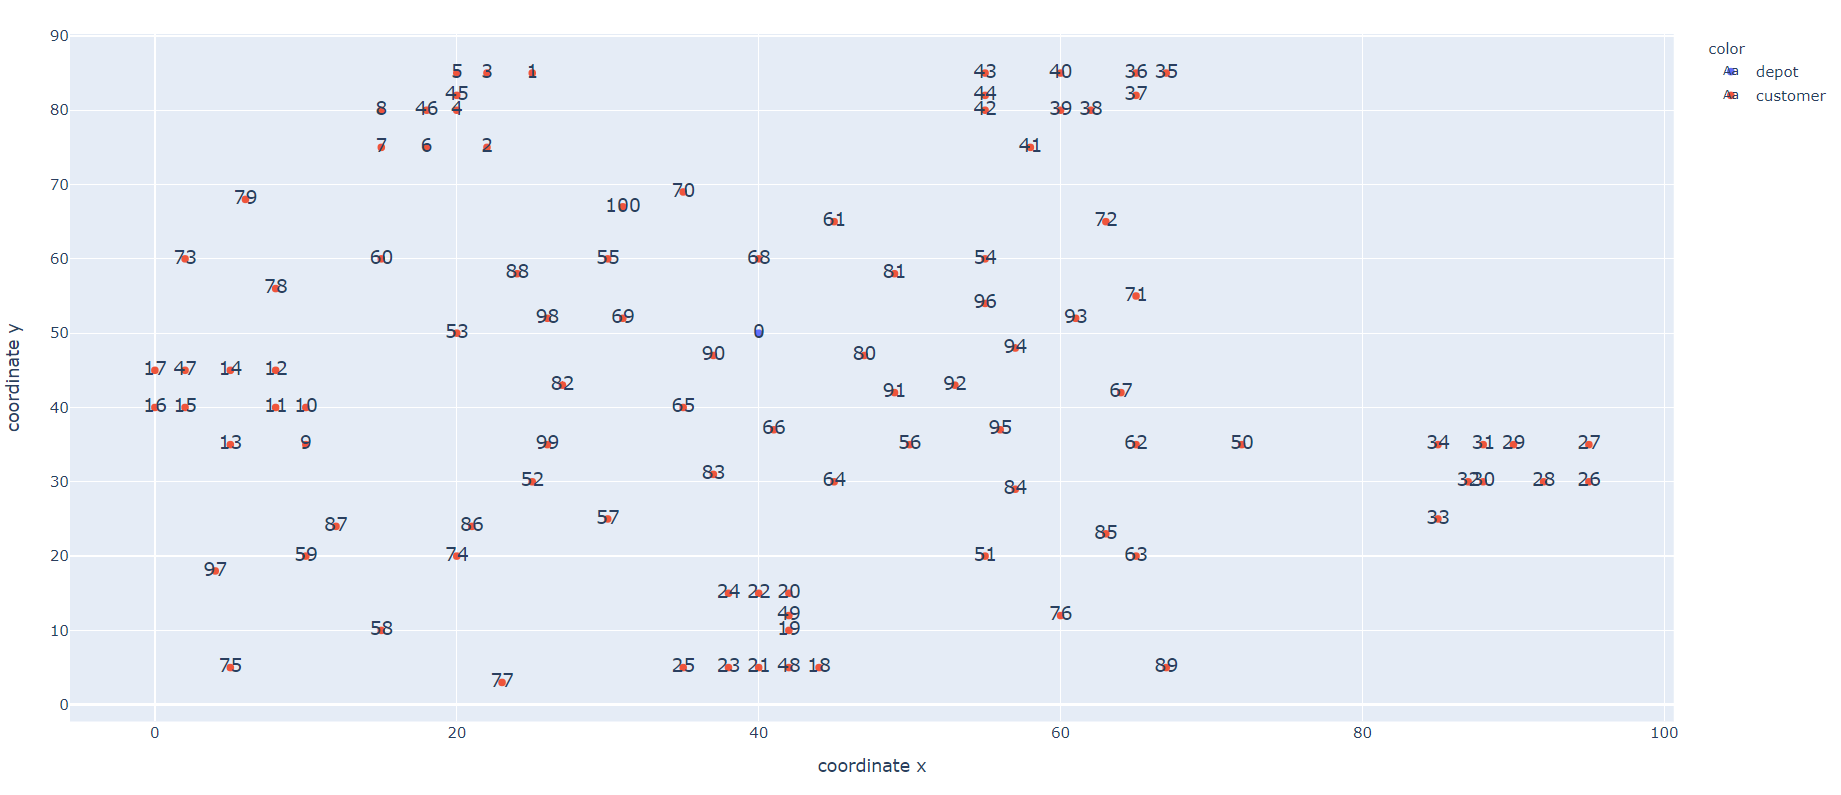
\includegraphics[width=\linewidth]{./img/aumman.png}
	\caption{Map of customers and depot}
	\label{map}
\end{figure}\

However, the customer may prefer a cost allocations which distributes cost equally. The Equal Profit Method and the Lorenz allocation were used to propose two different allocations. Table \ref{EPM} gathers the cost allocation computed with the Equal Profit Method, which took 6 second to be computed. The average cost for each customer is 16.94 money units and the EPM varies from 8.49 to 37.39 and its standard deviation is 6.07. Table \ref{Lorenz} shows the cost allocations computed with Lorenz allocation, which took 7 second to find a solution. This allocation varies from to and its standard deviation is 4.42.

To sum up, three allocation rules were considered to distribute the cost of these fictitious example. It turns out that the Aumann-Dr\`eze's value is the one which takes longer to compute and that it allocates cost based on the distance between customers and the depot. On the other hand, both EPM and Lorenz allocations take less time to compute and they distribute the cost equally. In these example the Lorenz allocation in the one which divides cost more equally between customers.
\clearpage
\begin{table}[H]
	\centering
	\begin{tabular}{c| c |c |c |c|c|c|c}
		\hline 
		%	\centering		
		$i$ customer & $\alpha_i$ & $i$ customer & $\alpha_i$ & $i$ customer & $\alpha_i$& $i$ customer & $\alpha_i$\\
		\hline
		1 & 15.48 & 2 & 16.14 & 3 & 16.0 & 4 & 14.66 \\
		5 & 21.12 & 6 & 13.54 & 7 & 18.52 & 8 & 15.87 \\
		9 & 13.01 & 10 & 12.27 & 11 & 14.71 & 12 & 14.21 \\
		13 & 14.78 & 14 & 13.72 & 15 & 15.25 & 16 & 16.0 \\
		17 & 15.64 & 18 & 18.53 & 19 & 16.43 & 20 & 14.38 \\
		21 & 23.69 & 22 & 14.36 & 23 & 18.48 & 24 & 18.46 \\
		25 & 23.84 & 26 & 16.05 & 27 & 15.04 & 28 & 14.98 \\
		29 & 2.19 & 30 & 16.43 & 31 & 14.49 & 32 & 16.86 \\
		33 & 27.1 & 34 & 14.72 & 35 & 17.57 & 36 & 17.09 \\
		37 & 16.14 & 38 & 14.79 & 39 & 14.33 & 40 & 16.02 \\
		41 & 28.2 & 42 & 31.3 & 43 & 15.13 & 44 & 14.05 \\
		45 & 19.77 & 46 & 15.12 & 47 & 14.87 & 48 & 23.72 \\
		49 & 15.61 & 50 & 13.67 & 51 & 21.51 & 52 & 15.6 \\
		53 & 31.19 & 54 & 10.83 & 55 & 7.41 & 56 & 21.58 \\
		57 & 16.8 & 58 & 20.69 & 59 & 18.61 & 60 & 17.47 \\
		61 & 14.75 & 62 & 18.7 & 63 & 25.05 & 64 & 12.87 \\
		65 & 4.9 & 66 & 15.6 & 67 & 16.23 & 68 & 5.86 \\
		69 & 5.98 & 70 & 7.81 & 71 & 20.21 & 72 & 21.69 \\
		73 & 25.5 & 74 & 22.5 & 75 & 25.01 & 76 & 22.61 \\
		77 & 37.39 & 78 & 21.13 & 79 & 20.15 & 80 & 10.18 \\
		81 & 14.32 & 82 & 6.48 & 83 & 7.89 & 84 & 17.33 \\
		85 & 22.75 & 86 & 20.1 & 87 & 16.76 & 88 & 11.61 \\
		89 & 27.63 & 90 & 5.08 & 91 & 7.72 & 92 & 9.22 \\
		93 & 12.67 & 94 & 10.28 & 95 & 12.87 & 96 & 9.33 \\
		97 & 21.13 & 98 & 5.49 & 99 & 12.81 & 100 & 7.82 \\
		\hline 
	\end{tabular} \
	\caption{Equal profit method cost allocation per customer}
	\label{EPM}
\end{table}\

\begin{table}[H]
	\centering
	\begin{tabular}{c| c |c |c |c|c|c|c}
		\hline 
		%	\centering		
		$i$ customer & $\alpha_i$ & $i$ customer & $\alpha_i$ & $i$ customer & $\alpha_i$& $i$ customer & $\alpha_i$\\
		\hline
		1 & 12.1 & 2 & 15.57 & 3 & 11.87 & 4 & 11.87 \\
		5 & 15.57 & 6 & 18.08 & 7 & 15.57 & 8 & 20.83 \\
		9 & 13.44 & 10 & 13.44 & 11 & 15.83 & 12 & 15.83 \\
		13 & 13.47 & 14 & 13.44 & 15 & 13.44 & 16 & 13.44 \\
		17 & 13.47 & 18 & 15.09 & 19 & 15.09 & 20 & 15.09 \\
		21 & 22.95 & 22 & 15.09 & 23 & 15.09 & 24 & 22.95 \\
		25 & 22.95 & 26 & 13.46 & 27 & 13.46 & 28 & 13.46 \\
		29 & 13.46 & 30 & 13.46 & 31 & 13.46 & 32 & 13.46 \\
		33 & 26.15 & 34 & 13.46 & 35 & 14.77 & 36 & 14.77 \\
		37 & 14.77 & 38 & 14.77 & 39 & 14.77 & 40 & 14.77 \\
		41 & 28.2 & 42 & 25.5 & 43 & 14.77 & 44 & 14.77 \\
		45 & 15.57 & 46 & 11.87 & 47 & 13.44 & 48 & 22.95 \\
		49 & 15.09 & 50 & 13.46 & 51 & 18.47 & 52 & 14.39 \\
		53 & 31.19 & 54 & 10.78 & 55 & 15.57 & 56 & 14.21 \\
		57 & 16.11 & 58 & 15.83 & 59 & 15.83 & 60 & 16.34 \\
		61 & 20.55 & 62 & 18.47 & 63 & 18.47 & 64 & 14.39 \\
		65 & 15.83 & 66 & 19.56 & 67 & 18.47 & 68 & 15.57 \\
		69 & 16.34 & 70 & 14.77 & 71 & 20.21 & 72 & 21.69 \\
		73 & 16.34 & 74 & 20.31 & 75 & 15.83 & 76 & 22.95 \\
		77 & 37.39 & 78 & 16.34 & 79 & 15.57 & 80 & 13.46 \\
		81 & 14.32 & 82 & 15.83 & 83 & 15.09 & 84 & 18.47 \\
		85 & 18.47 & 86 & 14.39 & 87 & 15.83 & 88 & 16.34 \\
		89 & 26.15 & 90 & 8.49 & 91 & 18.47 & 92 & 14.39 \\
		93 & 10.78 & 94 & 10.78 & 95 & 14.39 & 96 & 10.78 \\
		97 & 15.83 & 98 & 13.44 & 99 & 14.39 & 100 & 11.87	\\	
		\hline 
	\end{tabular} \
	\caption{Lorenz allocation per customer}
	\label{Lorenz}
\end{table}\




%=========================================================
%
%----------------------------------------------------------------------------------------
%	THESIS CONCLUSIONS
%----------------------------------------------------------------------------------------
%
% And the conclusions goes here
\chapter{Conclusiones}\label{chap:Conclusion}

\initial{T}his Master thesis proposes a metaheuristic which combines three local searches and a random sampling for the vehicle routing problem with capacity and time window constraints. Experimental results demonstrate its effectiveness, which matches 10 the 56 best published solutions to the Solomon benchmarks. It also gives good results to a real agricultural cooperative problem. The thesis also includes a robustness analysis which has shown the good metaheuristic's behavior.

The main cooperative game theory results are described as well as some of the best known allocation rules such as Shapley value, Aumann-Dr\`eze value, Equal profit method and Lorenz allocation. Cooperative routing problem is also introduced, focusing on the most common techniques to allocate its costs. Finally, two collaborative routing problem data sets are selected to be solved. This work allocated the cost using allocating rules, which turned out the different allocation rules behavior.

To sum up, this Master Thesis deals with the vehicle routing problem with time windows and its cost allocation.


%
% Apparently the guidelines don't say anything about citations or
% bibliography styles so I guess we can use anything.
\backmatter


%=========================================================
%
%----------------------------------------------------------------------------------------
%	THESIS CONTENT - APPENDICES
%----------------------------------------------------------------------------------------
%
% And the appendix goes here
\appendix
\chapter{Ap�ndice A}
\label{app:app01}

\initial{A}qu� empezar�a el primer ap�ndice si es que es necesario.


%----------------------------------------------------------------------------------------
%	BIBLIOGRAPHY
%----------------------------------------------------------------------------------------
\begin{thebibliography}{99}  % Un ejemplo de c�mo poner las referencias de forma manual. Para manejar muchas referencias no dudar en usar BibTeX
	%% \bibitem must have the following form:+
	\bibitem{ambro} Ambrosino, D., \& Sciomachen, A. (2007). A food distribution network problem: a case study. IMA Journal of Management Mathematics, 18(1), 33-53.
	
	\bibitem{Arin} Arin Aguirre, F. J. (2003). Egalitarian distributions in coalitional models: The Lorenz criterion.
	
	\bibitem{Aumann} Aumann, R. J., \& Dreze, J. H. (1974). Cooperative games with coalition structures. International Journal of game theory, 3(4), 217-237.
	
	\bibitem{Agarwal} Agarwal, R., \& Ergun, �. (2010). Network design and allocation mechanisms for carrier alliances in liner shipping. Operations research, 58(6), 1726-1742.
	
	\bibitem{Backer} De Backer, B., Furnon, V., Shaw, P., Kilby, P. \& Prosser, P. (2000). Solving vehicle routing problems using constraint programming and metaheuristics. Journal of Heuristics, 6(4), 501-523.
	
	\bibitem{Berger} Berger, J., Barkaoui, M. \& Br\"aysy, O. (2001). A parallel hybrid genetic algorithm for the vehicle routing problem with time windows. Working paper, Defense Research Establishment Valcartier.
	
	\bibitem{bra} Br\"aysy, O. \& Gendreau, M. (2001). Route construction and local search algorithms for the vehicle routing problem with time windows. Sintef Report, STF42 A, 1024.
	
	\bibitem{bra2} Br\"aysy, O. (2001). Local search and variable neighborhood search algorithms for the vehicle routing problem with time windows. Vaasan yliopisto.
	
	\bibitem{Bent} Bent, R. \& Van Hentenryck, P. (2004). A two-stage hybrid local search for the vehicle routing problem with time windows. Transportation Science, 38(4), 515-530.
	
	\bibitem{Chiang} Chiang, W. C. \& Russell, R. A. (1996). Simulated annealing metaheuristics for the vehicle routing problem with time windows. Annals of Operations Research, 63(1), 3-27.
	
	\bibitem{Chiang2} Chiang, W. C. \& Russell, R. A. (1997). A reactive tabu search metaheuristic for the vehicle routing problem with time windows. INFORMS Journal on computing, 9(4), 417-430.
	
	\bibitem{Clark} Clarke, G. \& Wright, J. W. (1964). Scheduling of vehicles from a central depot to a number of delivery points. Operations research, 12(4), 568-581.
	
	\bibitem{Czech} Czech, Z. J. \& Czarnas, P. (2002, January). Parallel simulated annealing for the vehicle routing problem with time windows. In euromicro-pdp (p. 0376). IEEE.
	
	\bibitem{Cordeau} Cordeau, J. F., Laporte, G. \& Mercier, A. (2001). A unified tabu search heuristic for vehicle routing problems with time windows. Journal of the Operational research society, 52(8), 928-936.
	
	\bibitem{Ballot} Ballot, E., \& Fontane, F. (2010). Reducing transportation CO2 emissions through pooling of supply networks: perspectives from a case study in French retail chains. Production Planning \& Control, 21(6), 640-650.
	
	%de Frutos, R. M. G. \& Casas-M\'endez, B. V. (2016). A hybrid heuristic algorithm with application to a graphical interface for vehicle routing optimization in an agricultural cooperative. arXiv preprint arXiv:1607.02377.
	
	
	\bibitem{Dantzig} Dantzig, G. B., \& Ramser, J. H. (1959). The truck dispatching problem. Management science, 6(1), 80-91.
	
	% Agnieszka Debudaj-Grabysz, Zbigniew J.Czech and Piotr Czarnas Silesia, 2004. University of Technology and University of Wroclaw, Poland.
	
	\bibitem{Fisher} Fisher, M. L., J�rnsten, K. O. \& Madsen, O. B. (1997). Vehicle routing with time windows: Two optimization algorithms. Operations research, 45(3), 488-492.
	
	\bibitem{Frisk} Frisk, M., G�the-Lundgren, M., J�rnsten, K., \& R�nnqvist, M. (2010). Cost allocation in collaborative forest transportation. European Journal of Operational Research, 205(2), 448-458.
	
	\bibitem{Gambardella} Gambardella, L. M., Taillard, \'E. \& Agazzi, G. (1999). Macs-vrptw: A multiple colony system for vehicle routing problems with time windows. In New ideas in optimization.
	
	\bibitem{Gansterer} Gansterer, M., \& Hartl, R. F. (2018). Collaborative vehicle routing: a survey. European Journal of Operational Research, 268(1), 1-12.
	
	\bibitem{Golden } Golden, B. L., \& Assad, A. A. (1986). Vehicle routing with time-window constraints: Algorithmic solutions (Vol. 15). Amer Sciences Press.
	% Golden is not used
	
	\bibitem{Balbina} Roque M. Guiti\'an de Frutos, Balbina V. Casas-M \'endez, (2016). (To appear). Routing problems in agricultural cooperatives: A model for optimization of transport vehicle logistics IMA Journal of Management Mathematics. DOI:10.1093/imaman/dpy010.
	
	
	\bibitem{Harsanyi} Harsanyi, J. C. (1966). A general theory of rational behavior in game situations. Econometrica: Journal of the Econometric Society, 613-634.
	\bibitem{Helsgaun} Helsgaun, K., (1998). An Effective Implementation of the Lin-Kernighan Traveling Salesman Heuristic. Datalogiske Skrifter (Writings on Computer Science), No. 81.
	
	\bibitem{Homberger} Homberger, J. (2000). Eine verteilt-parallele Metaheuristik. In Verteilt-parallele Metaheuristiken zur Tourenplanung (pp. 139-165). Deutscher Universit\"atsverlag, Wiesbaden.
	% Golden is not used
	\bibitem{Gehring} Homberger, J. \& Gehring, H. (1999). Two evolutionary metaheuristics for the vehicle routing problem with time windows. INFOR: Information Systems and Operational Research, 37(3), 297-318.
	
	\bibitem{Kimms} Kimms, A., \& Kozeletskyi, I. (2016). Shapley value-based cost allocation in the cooperative traveling salesman problem under rolling horizon planning. EURO Journal on Transportation and Logistics, 5(4), 371-392.
	
	% T. Ibaraki, M. Kubo, T. Masuda, T. Uno and M. Yagiura, 2001. "Effective Local Search Algorithms for the Vehicle Routing Problem with General Time Windows," Working Paper, Department of Applied Mathematics and Physics, Kyoto University, Japan.
	
	\bibitem{Juan} Juan, A. A., Faulin, J., Ruiz, R., Barrios, B., Gilibert, M. \& Vilajosana, X. (2009). Using oriented random search to provide a set of alternative solutions to the capacitated vehicle routing problem. In Operations research and cyber-infrastructure (pp. 331-345). Springer, Boston, MA.
	
	\bibitem{Lenstra} Lenstra, J. K. \& Kan, A. R. (1981). Complexity of vehicle routing and scheduling problems. Networks, 11(2), 221-227.
	
	\bibitem{cluster} MacQueen, J. (1967, June). Some methods for classification and analysis of multivariate observations. In Proceedings of the fifth Berkeley symposium on mathematical statistics and probability (Vol. 1, No. 14, pp. 281-297).
	
	\bibitem{bra3} Mester, D., Br\"aysy, O. \& Dullaert, W. (2007). A multi-parametric evolution strategies algorithm for vehicle routing problems. Expert Systems with Applications, 32(2), 508-517.
	
	% \bibitem{Li-Lim} Li, H., Lim, A. \& Huang, J. (2001). Local Search with Annealing-like Restarts to Solve the VRPTW. Working Paper, Department of Computer Science, National University of Singapore.
	
	\bibitem{L-K} Lin, S., Kernighan, B. W. (1973). An Effective Heuristic Algorithm for the Traveling-Salesman Problem. Operations research. 21, 498-516.
	
	\bibitem{Neumann} Neumann, J. O. H. N., \& Morgenstern, O. S. K. A. R. (1944). Theory of Games and Economic Behaviour Princeton Univ. Press, Princeton.
	\bibitem{Potvin1996} Potvin, J. Y. \& Bengio, S. (1996). The vehicle routing problem with time windows part II: genetic search. INFORMS journal on Computing, 8(2), 165-172.
	
	\bibitem{Rousseau} Rousseau, L. M., Gendreau, M. \& Pesant, G. (2002). Using constraint-based operators to solve the vehicle routing problem with time windows. Journal of heuristics, 8(1), 43-58.
	
	%  S. Ropke,  D.Pisinger. "A general heuristic for vehicle routing problems",  technical report, Department of Computer Science, University of Copenhagen.
	
	\bibitem{Rochat} Rochat, Y. \& Taillard, \'E. D. (1995). Probabilistic diversification and intensification in local search for vehicle routing. Journal of heuristics, 1(1), 147-167.
	
	% Hasle G., O. Kloster, 2007. "Industrial Vehicle Routing Problems". Chapter in Hasle G., K-A Lie, E. Quak (eds): Geometric Modelling, Numerical Simulation, and Optimization. ISBN 978-3-540-68782-5, Springer.
	
	%  G. Schrimpf, J. Schneider, H. Stamm-Wilbrandt and G. Dueck, 2000. "Record Breaking Optimization Results Using the Ruin and Recreate Principle," Journal of Computational Physics 159, 139-171.
	\bibitem{Schmeidler} Schmeidler, D. (1969). The nucleolus of a characteristic function game. SIAM Journal on applied mathematics, 17(6), 1163-1170.
	
	\bibitem{Shapley} Shapley, L. S. (1953). A value for n-person games. Contributions to the Theory of Games, 2(28), 307-317.
	
	\bibitem{Shaw1} Shaw, P. (1997). A new local search algorithm providing high quality solutions to vehicle routing problems. APES Group, Dept of Computer Science, University of Strathclyde, Glasgow, Scotland, UK.
	
	\bibitem{Shaw2} Shaw, P. (1998, October). Using constraint programming and local search methods to solve vehicle routing problems. In International conference on principles and practice of constraint programming (pp. 417-431). Springer, Berlin, Heidelberg.
	
	\bibitem{Solomon_1987} Solomon, M. M. (1987). Algorithms for the vehicle routing and scheduling problems with time window constraints. Operations research, 35(2), 254-265.
	
	
	\bibitem{Taillard} Taillard, E., Badeau, P., Gendreau, M., Geurtin, F. \& Potvin, J.Y., (1997). A Tabu Search Heuristic for the Vehicle Routing Problem with Time Windows," Transportation Science, 31, 170-186.
	
	\bibitem{Woch} Woch, M. \& \L{}ebkowski, P. (2009). Sequential simulated annealing for the vehicle routing problem with time windows. Decision Making in Manufacturing and Services, 3(1-2), 87-100.
	
	\bibitem{Zon} van Zon, M. A., \& van den Heuvel, W. (2017). Cost allocation in cooperative transport: The joint network vehicle routing game.
	
\end{thebibliography}

%
% Add index
%\printindex
%   
\end{document}